\documentclass[masc,grad]{coppe} %Universal input encoding G.L.
% \documentclass[aprovado,masc,grad]{coppe} %Universal input encoding G.L.
\maxdeadcycles=20
\usepackage[utf8]{inputenc}
\usepackage[english]{babel}
% \usepackage[brazil]{babel}
\usepackage[T1]{fontenc}
\usepackage{graphicx}
\usepackage{pax}
\usepackage{tikzscale}
\usepackage{appendix}
\usepackage{pgfplots}
\pgfplotsset{compat=newest}
\usepgfplotslibrary{groupplots}
\usepgfplotslibrary{dateplot}
\usepackage{xargs}
\usepackage{rotating}
\usepackage{pdflscape}
\usepackage{afterpage}
\usepackage[paper=A4,pagesize]{typearea}
\graphicspath{{../../figures/}} 
\usepackage{subcaption} 
\usepackage{hyperref}
\usepackage{amsmath,amssymb} 
\usepackage{indentfirst}
\usepackage[algo2e,linesnumbered,ruled]{algorithm2e}
\usepackage{algorithmic}
%%If desirable, the user can enable Times New Roman Fonts by uncommenting the next line. G.L.
% \usepackage{mathptmx}
\usepackage{pdfpages}
\usepackage{multirow}
\usepackage{color}
\usepackage{blindtext}
\usepackage{float}
\usepackage{nameref}
\usepackage{cleveref}
\usepackage{multicol}
\usepackage{listings}
\usepackage{enumerate}
\usepackage[acronym,toc]{glossaries}\makeglossaries
\usepackage{tikz}
\usepackage{ladder} %https://github.com/AurelienC/tex-ladder/blob/master/ladder.sty
\usetikzlibrary{arrows,shapes,automata,petri,external,arrows.meta}
	\tikzset{
	place/.style={
	circle,
	thick,
	draw=black!100, % draw=blue!75,
    % fill=blue!20,
    minimum size=6mm
  },
  extPlace/.style={
    circle,
    dotted,
    draw=black!100, % draw=blue!75,
    % fill=blue!20,
    minimum size=6mm
  },
  extTransition/.style={
    rectangle,
    dotted,
    fill=white,
    minimum width=8mm,
    inner ysep=0.7pt
  },
  transition/.style={
    rectangle,
    thick,
    fill=black,
    minimum width=8mm,
    inner ysep=0.7pt
  },
  extTimedtransition/.style={
    rectangle,
    dotted,
    fill=white,
    minimum width=8mm,
    inner ysep=2pt
  },
  timedtransition/.style={
    rectangle,
    thick,
    fill=white,
    minimum width=8mm,
    inner ysep=2pt
  },
  inhibitor/.style={-o},
  text/.style={}
}

\makeatletter
\tikz@def@grow@tokens{2}{1}{-1.5}{0}
\tikz@def@grow@tokens{2}{2}{1.5}{0}
% \tikz@def@grow@tokens{3}{1}{-1}{0}
% \tikz@def@grow@tokens{3}{2}{0}{1}
% \tikz@def@grow@tokens{3}{3}{1.5}{-1}
\makeatother


\definecolor{darkblue}{rgb}{0,0,0.3}
\definecolor{blue}{rgb}{0,0,0.5}
\definecolor{color1}{rgb}{1,0.2,0.3}
\definecolor{color2}{rgb}{0.05490196078,0.41176470588,0.13333333333}
% rgb(14, 105, 34)

\definecolor{color3}{rgb}{0.2,0.2,0.8}
% hyperref setup
\hypersetup{
  % pdftitle={\title},
  pdfauthor={Rafael Accácio Nogueira},
  pdfcreator={Rafael Accácio Nogueira},     
  bookmarksopen=true,         
  bookmarksopenlevel=1,       
  colorlinks=true, % false => boxes 
  linkcolor=blue,
  filecolor=red,  
  urlcolor=blue,  
  citecolor=blue,              
  pdfstartview=Fit,          
  pdfpagemode=UseOutlines,    % this is the option you were lookin for
  pdfpagelayout=TwoPageRight,
}

\makeatletter
\let\stdchapter\chapter
\renewcommand*\chapter{%
  \@ifstar{\starchapter}{\@dblarg\nostarchapter}}
\newcommand*\starchapter[1]{\stdchapter*{#1}}
\def\nostarchapter[#1]#2{
  \stdchapter[#1]{\protect\hyperlink{tocsection}{#1}}}
\makeatother

\makeatletter
\let\stdsection\section
\renewcommand*\section{%
  \@ifstar{\starsection}{\@dblarg\nostarsection}}
\newcommand*\starsection[1]{\stdsection*{#1}}
\def\nostarsection[#1]#2{
  \stdsection[#1]{\protect\hyperlink{tocsection}{#1}}}
\makeatother

\makeatletter
\let\stdsubsection\subsection
\renewcommand*\subsection{%
  \@ifstar{\starsubsection}{\@dblarg\nostarsubsection}}
\newcommand*\starsubsection[1]{\stdsubsection*{#1}}
\def\nostarsubsection[#1]#2{
  \stdsubsection[#1]{\protect\hyperlink{tocsection}{#1}}}
\makeatother

\makeatletter
\let\stdsubsubsection\subsubsection
\renewcommand*\subsubsection{%
  \@ifstar{\starsubsubsection}{\@dblarg\nostarsubsubsection}}
\newcommand*\starsubsubsection[1]{\stdsubsubsection*{#1}}
\def\nostarsubsubsection[#1]#2{
  \stdsubsubsection[#1]{\protect\hyperlink{tocsection}{#1}}}
\makeatother

\let\oldtoc\tableofcontents
\renewcommand{\tableofcontents}{\pagebreak\hypertarget{tocsection}{}\label{tocsection}\oldtoc}


\newcommand{\figplaceholder}[2]{
	\begin{figure}[H]
		\begin{center}	
			\rule{8cm}{8cm}
			\caption{\todo[FORGOT TO INCLUDE FIGURE]{#1 (placeholder)}}
			\label{fig:#2}
		\end{center}
	\end{figure}
}

\newif\ifdebug
\newcommand{\draft}{\debugtrue}
\newcommand{\final}{\debugfalse}
\newcommand{\todo}[2][FORGOT TO DO SOMETHING]{\ifdebug {\color{red}#2}\else \PackageError{}{#1}{}\fi}
\newcommand\doing[1]{\ifdebug {\color{blue}#1}\else \PackageError{}{FORGOT TO DO SOMETHING}{}\fi}
\newcommand\warning[1]{\ifdebug {\color{red}#1}\fi}
\newcommand\note[1]{\ifdebug {\color{orange}#1}\fi}

\usepackage{fancyhdr}
\pagestyle{fancy}

\fancyhead[L]{\warning{DRAFT}}
\fancyhead[R]{\warning{DEBUG ON}}

\fancyfoot[L]{\warning{TURN DEBUG OFF}}
\fancyfoot[R]{\warning{DRAFT}}

\newtheorem{theorem}{Theorem}
\numberwithin{theorem}{chapter}

\newtheorem{example}{Example}
\numberwithin{example}{chapter}

\newtheorem{definition}{Definition}
\numberwithin{definition}{chapter}

\newtheorem{observation}{Remark}
\numberwithin{observation}{chapter}

\usepackage[export]{adjustbox}

\newcommand{\includetikzfigure}[2][]{
    \ifdebug {\includegraphics[#1]{#2.pdf}}
    \else  \includegraphics[#1]{#2}\fi
}

\newcommand{\addtikzfigureLandscape}[4][width=0.8\textwidth]{
\KOMAoptions{paper=landscape}
\recalctypearea
  \vspace*{\fill}
  \begin{figure}[H]
    \centering
    \ifdebug {\includegraphics[#1]{#2.pdf}}
    \else  \includegraphics[#1]{#2}\fi
    \caption{#3}
    \label{fig:#4}
  \end{figure}
  \vspace*{\fill}
\KOMAoptions{paper=portrait}
\recalctypearea
}

\newcommand{\addtikzfigureLandscapeAthree}[4][width=0.8\textwidth]{
\KOMAoptions{paper=a3,paper=landscape}
% \KOMAoptions{paper=landscape}
\recalctypearea
  \begin{figure}[H]
    \vspace{-2cm}
    \centering
    \ifdebug {\centerline{\includegraphics[#1]{#2.pdf}}}
    \else  \centerline{\includegraphics[#1]{#2}}
\fi
    % \caption{#3}
    % \label{fig:#4}
  \end{figure}
\KOMAoptions{paper=a4,paper=portrait}
\recalctypearea
}

% \newcommand{\addtikzfigureVertCent}[3]{
% \KOMAoptions{paper=landscape}
% \recalctypearea
% % \begin{landscape}
% \vspace*{\fill}
%   \begin{figure}[H]
%     % \centering
%     % \resizebox{\hsize}{!}{
%     % \input{#1}
%      \includegraphics[width=1.15\textwidth]{#1}
%     % }
%     \caption{#2}
%     \label{fig:#3}
%   \end{figure}
% \vspace*{\fill}
% % \end{landscape}
% \KOMAoptions{paper=portrait}
% \recalctypearea
% }

\newcolumntype{P}[1]{>{\centering\arraybackslash}p{#1}}
\newcolumntype{M}[1]{>{\centering\arraybackslash}m{#1}}
\definecolor{keywordstyle}{rgb}{0,0,0.82}
\definecolor{commentstyle}{rgb}{0,0.6,0}
\definecolor{numberstyle}{rgb}{0.5,0.5,0.5}
\definecolor{stringstyle}{rgb}{0.58,0,0.82}

% Listing options
\lstset{ 
  % backgroundcolor=\color{white},   % choose the background color; you must add \usepackage{color} or \usepackage{xcolor}; should come as last argument
  basicstyle=\footnotesize,        % the size of the fonts that are used for the code
  breakatwhitespace=false,         % sets if automatic breaks should only happen at whitespace
  breaklines=true,                 % sets automatic line breaking
  captionpos=t,                    % sets the caption-position to bottom
  commentstyle=\color{commentstyle},    % comment style
  deletekeywords={...},            % if you want to delete keywords from the given language
  escapeinside={\%*}{*)},          % if you want to add LaTeX within your code
  extendedchars=true,              % lets you use non-ASCII characters; for 8-bits encodings only, does not work with UTF-8
  % firstnumber=1000,                % start line enumeration with line 1000
  % frame=single,	                   % adds a frame around the code
  keepspaces=true,                 % keeps spaces in text, useful for keeping indentation of code (possibly needs columns=flexible)
  keywordstyle=\color{keywordstyle},       % keyword style
  % language=Octave,                 % the language of the code
  morekeywords={*,...},            % if you want to add more keywords to the set
  numbers=left,                    % where to put the line-numbers; possible values are (none, left, right)
  numbersep=10pt,                   % how far the line-numbers are from the code
  numberstyle=\tiny\color{numberstyle}, % the style that is used for the line-numbers
  rulecolor=\color{black},         % if not set, the frame-color may be changed on line-breaks within not-black text (e.g. comments (green here))
  showspaces=false,                % show spaces everywhere adding particular underscores; it overrides 'showstringspaces'
  showstringspaces=false,          % underline spaces within strings only
  showtabs=false,                  % show tabs within strings adding particular underscores
  stepnumber=2,                    % the step between two line-numbers. If it's 1, each line will be numbered
  stringstyle=\color{stringstyle},     % string literal style
  tabsize=2,	                   % sets default tabsize to 2 spaces
  title=\lstname                   % show the filename of files included with \lstinputlisting; also try caption instead of title
}

%% as seen in https://tex.stackexchange.com/a/183682/143332
\makeatletter
\newcommand\Autoref[1]{\@first@ref#1,@}
\def\@throw@dot#1.#2@{#1}% discard everything after the dot
\def\@set@refname#1{%    % set \@refname to autoefname+s using \getrefbykeydefault
    \edef\@tmp{\getrefbykeydefault{#1}{anchor}{}}%
    \xdef\@tmp{\expandafter\@throw@dot\@tmp.@}%
    \ltx@IfUndefined{\@tmp autorefnameplural}%
         {\def\@refname{\@nameuse{\@tmp autorefname}s}}%
         {\def\@refname{\@nameuse{\@tmp autorefnameplural}}}%
}
\def\@first@ref#1,#2{%
  \ifx#2@\autoref{#1}\let\@nextref\@gobble% only one ref, revert to normal \autoref
  \else%
    \@set@refname{#1}%  set \@refname to autoref name
    \@refname~\ref{#1}% add autoefname and first reference
    \let\@nextref\@next@ref% push processing to \@next@ref
  \fi%
  \@nextref#2%
}
\def\@next@ref#1,#2{%
   \ifx#2@ and~\ref{#1}\let\@nextref\@gobble% at end: print and+\ref and stop
   \else, \ref{#1}% print  ,+\ref and continue
   \fi%
   \@nextref#2%
 }
 \makeatother

\newcommand{\colvec}[2][1]{%
  \scalebox{#1}{%
    \renewcommand{\arraystretch}{.7}%
    $\begin{bmatrix}#2\end{bmatrix}$%
  }
}


%%% Local Variables:
%%% mode: latex
%%% TeX-master: "./monografia.tex"
%%% End:

% \usepackage{fontspec}
% \usepackage{fontawesome}
\newcommandx\acr[5][4=,5=]{
  \ifthenelse{\equal{#5}{}}
  {
    \acrSing{#1}{#2}{#3}
  }
  {
    \acrPl{#1}{#2}{#3}{#4}{#5}
  }
  } 

\newcommand{\acrSing}[3]{\newacronym{#1}{#2}{#3}
  \expandafter\newcommand\csname #1\endcsname{\gls{#1}}}

\newcommand{\acrPl}[5]{
  \newacronym[plural=#4,firstplural=#5 (#4)]{#1}{#2}{#3}
  \expandafter\newcommand\csname #1\endcsname{\gls{#1}}
  \expandafter\newcommand\csname #4\endcsname{\glspl{#1}}
}

\renewcommand{\symbl}[3]{\newglossaryentry{#1}{name ={#2},	description ={#3}}
  \expandafter\newcommand\csname #1\endcsname{\gls{#1}}
}


\newglossarystyle{dottedlocations}{%
   \glossarystyle{list}%
   \renewcommand*{\glossaryentryfield}[5]{%
   \item[\glsentryitem{##1}\glstarget{##1}{##2}] ##3, p %
       \unskip\leaders\hbox to 2.9mm{} ##5}%
   \renewcommand*{\glsgroupskip}{}%
}

 \newglossarystyle{acronyms}{%
 % put the glossary in the itemize environment:
 \renewenvironment{theglossary}%
   {\begin{tabbing}}{\end{tabbing}}%
 % have nothing after \begin{theglossary}:
 \renewcommand*{\glossaryheader}{}%
 % have nothing between glossary groups:
 \renewcommand*{\glsgroupheading}[1]{}%
 \renewcommand*{\glsgroupskip}{}%
 % set how each entry should appear:
 \renewcommand*{\glossentry}[2]{%
 \glstarget{##1}{\glossentryname{##1}}\\% \kill % the entry name
 \=\glossentrysymbol{##1}% the symbol in brackets
 \space \glossentrydesc{##1},% the description
 \space p. ##2\\% the number list in square brackets
 }%
 % set how sub-entries appear:
 \renewcommand*{\subglossentry}[3]{%
   \glossentry{##2}{##3}}%
}


 \newglossarystyle{symbols}{%
 % put the glossary in the itemize environment:
 \renewenvironment{theglossary}%
   {\begin{tabbing}}{\end{tabbing}}%
 % have nothing after \begin{theglossary}:
 \renewcommand*{\glossaryheader}{}%
 % have nothing between glossary groups:
 \renewcommand*{\glsgroupheading}[1]{}%
 \renewcommand*{\glsgroupskip}{}%
 % set how each entry should appear:
 \renewcommand*{\glossentry}[2]{%
 \glstarget{##1}{\glossentryname{##1}}\\% \kill % the entry name
 \=\textbf{\glossentrysymbol{##1}}% the symbol in brackets
 
 \space \glossentrydesc{##1},% the description
 \space p. ##2\\% the number list in square brackets
 }%
 % set how sub-entries appear:
 \renewcommand*{\subglossentry}[3]{%
   \glossentry{##2}{##3}}%
 }


\acr{DAOCT}{DAOCT}{Deterministic Automaton
  with Outputs and Conditional Transitions}
\acr{ECA}{ECA}{Engenharia de controle e Automação}
\acr{PLC}{PLC}{Programmable Logic Controller}
[PLCs][Programmable Logic Controllers]
\acr{DES}{DES}{Discrete Event System}
[DESs][Discrete Event Systems]


\acr{LD}{LD}{Ladder Diagram}

\acr{CIPN}{CIPN}{Control Interpreted Petri Net}

% DAOCT
\symbl{OmegaSet}{$\Omega$}{$\Omega \subset \mathbb{N}_1^{m_i + m_0}$ Set of IO vectors}
\symbl{SigmaSet}{$\Sigma$}{Set of events}
\symbl{XSet}{$X$}{Set of states}
\symbl{ffunction}{$f$}{$f : X \times \Sigma^* \rightarrow X$ Deterministic
  transition function}
\symbl{lambdafunction}{$\lambda$}{$\lambda : X \rightarrow \Omega$ State
  output function}
\symbl{RSet}{$R$}{$R = \{1,2,\dots,r\} $ Set of path indices}
\symbl{thetafunction}{$\theta$}{$\theta : X \times \Sigma \rightarrow 2^R$ Path
  estimation function}
\symbl{xZero}{$x_0$}{Initial State}
\symbl{XfSet}{$X_f$}{$X_f \subseteq X$ Set of final states}
%%% Local Variables:
%%% mode: latex
%%% TeX-master: "./monografia.tex"
%%% End:
\makeindex
\makelosymbols
\makeloabbreviations

% \final
\draft


\signedFrontPage{../../figures/poli-logo.pdf}



\title{Identification and Failure~Detection in a Didactic~Manufacture~System}
\foreigntitle{Identificação e Detecção~de~Falhas em um Sistema~de~Manufatura~Didático}
\author{Rafael Accácio}{Nogueira}
\advisor{Prof.}{Marcos Vicente de Brito}{Moreira}{D.Sc.}
% Case advisor is a woman add {f} Example:
% \advisor{Prof.}{Marie}{Sklodowksca-Curie}{PhD.}{f}

% \advisor{Prof.}{Nome do Segundo Orientador}{Sobrenome}{Ph.D.}
% \advisor{Prof.}{Nome do Terceiro Orientador}{Sobrenome}{D.Sc.}
\examiner{Prof.}{Marcos Vicente de Brito Moreira}{D.Sc.}
% \examiner{Prof.}{Fernando César Lizarralde}{D.Sc.}
% \examiner{Prof.}{Nome do Terceiro Examinador Sobrenome}{D.Sc.}
\department{ECA}

\date{04}{2019}
\keyword{Failure~Detection}
\keyword{Discrete~Event~Systems}

% \newfontfamily{\FA}{FontAwesome}
% \def\Github{{\FA \faGithub}}
% \href{http://github.com/Accacio}{\Github Accacio}

\tikzset{every node/.style={align=center}}

% include only to speed up tests
\includeonly{
  % frontMatter/frontMatter
  % ,test/examples
  % ,mainMatter/introduction
  % ,mainMatter/background
  % ,mainMatter/system
  % ,mainMatter/petriNets
  % ,mainMatter/results
  % ,mainMatter/conclusion
  % ,appendices/complete
  ,appendices/tools
}
\begin{document}

\maketitle
\frontmatter
\makefrontpage
\makecatalog
\dedication{“It's a dangerous business going out your door. You step onto the road,
and if you don't keep your feet, there's no knowing where you might be swept off
to.” \\(J.R.R Tolkien)}
% ``É um negócio perigoso, Frodo, sair da sua porta. Você pisa na estrada, e, se
% não controlar seus pés, não há como saber até onde você pode ser levado''
% ``Se enxerguei mais longe, foi porque me apoiei sobre os ombros de gigantes.'' (Isaac Newton)

%%% Local Variables:
%%% mode: latex
%%% TeX-master: "../monografia.tex"
%%% End:

\chapter*{Agradecimentos} Primeiramente a Deus, sem
quem nada é possível e por \mbox{\textbf{todas}} as pessoas colocadas em meu caminho, que
me fizeram crescer e ser o indivíduo que hoje sou.

Aos meus pais, Rosemeri e Rogério. Por todo amor, carinho, atenção e
apoio dados, pela primeira educação, essencial para toda minha
trajetória, educação não só acadêmica, mas também moral. Obrigado, por tudo ! Amo muito vocês.

A todas minhas professoras e professores por 
 mostrarem o quão importante e bonita é a profissão e por terem sempre
 instigado a sede pelo aprendizado. Agradeço àqueles que contribuíram para
 minha base acadêmica e profissional.

As amizades que fiz, as que se foram de minha convivência e
   as que permaneceram, agradeço aqueles que conheci na UFRJ, mais especificamente a nossa turma T17,
   pois se chegamos até onde chegamos foi porque estivemos juntos, fortes, ombro
   no ombro, tentando não deixar o outro cair, mas quando alguém caía
   sempre uma mão amiga se estendia para ajudar a levantar e recomeçar. 

Ao Paulo Yamasaki, pelo convívio no LABECA, e pelas
   trocas de ideias em assuntos gerais que por fim, intencionalmente ou não, se
   tornariam orientação em diversos projetos que fiz na faculdade, e até mesmo
   orientação acadêmica e profissional. 

Aos melhores companheiros de grupo, Gabriel Pelielo e Rodrigo Moysés, um
verdadeiro ``Power Trio''. Também a Philipe Moura e Felipe Matheus, que me
incentivaram a sair da minha zona de conforto e me fizeram compreender de fato o sentido do quão
``perigoso'' é sair pela porta de casa, pois quando saímos da nossa zona de
conforto, coisas mágicas podem acontecer e pessoas mágicas podem aparecer em
nossas vidas.

À Evelise, a pessoa mágica que apareceu em minha vida, que me ajudou
fisicamente e psicologicamente nos momentos que mais precisei. Obrigado por escolher compartilhar parte de sua
vida comigo e por toda a força dada para o término desse ciclo. Eu te amo!  

Por fim às pessoas que me ajudaram mais diretamente neste projeto, Ryan
Pitanga e ao meu orientador Marcos Moreira 

%%% Local Variables: mode: latex TeX-master: "../monografia.tex" End:

\begin{foreignabstract}

In this work, we present ...

\end{foreignabstract}
\begin{abstract}

Apresenta-se, nesta tese, ...

\end{abstract}

\tableofcontents
\pagebreak
\listoffigures
\listoftables

% \printlosymbols
% \printloabbreviations

\printglossary[style=acronyms,title=List of Acronyms,type=\acronymtype]\newpage
\printglossary[style=symbols,title=List of Symbols]



%%% Local Variables:
%%% mode: latex
%%% TeX-master: "../monografia"
%%% End:

\mainmatter

\chapter{Examples}
\label{chap:examples}

\section{teste}
\subsection{teste}
\subsubsection{teste}
\begin{figure}[H]
  \centering
  \begin{tikzpicture}
    \node[anchor=south west,inner sep=0] (image) at (0,0) {
      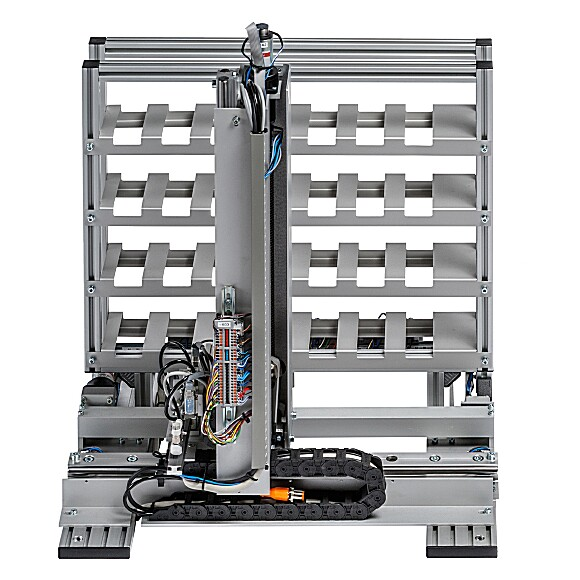
\includegraphics[width=8cm]{maquete/elevador/69523_3.jpg}
    };
    % \draw[red,ultra thick,rounded corners] (0,0) rectangle (9.4,6.2);
    \begin{scope}[x={(image.south east)},y={(image.north west)}]
        % \draw[help lines,xstep=.1,ystep=.1] (0,0) grid (1,1);
        % \foreach \x in {0,1,...,9} { \node [anchor=north] at (\x/10,0) {0.\x}; }
        % \foreach \y in {0,1,...,9} { \node [anchor=east] at (0,\y/10) {0.\y}; }
      \draw[red] (1,0.5) node {\textbf{Right}};
      \draw[red] (0,0.5) node {\textbf{Left}};
      \draw[red] (0.5,1) node {\textbf{Top}};
      \draw[red] (0.5,0) node {\textbf{Bottom}};
      \end{scope}
  \end{tikzpicture}
  \caption{Storage Unit}
\end{figure}


\begin{figure}[H]
  \centering
  \begin{tikzpicture}
    \node[anchor=south west,inner sep=0] (image) at (0,0) {
      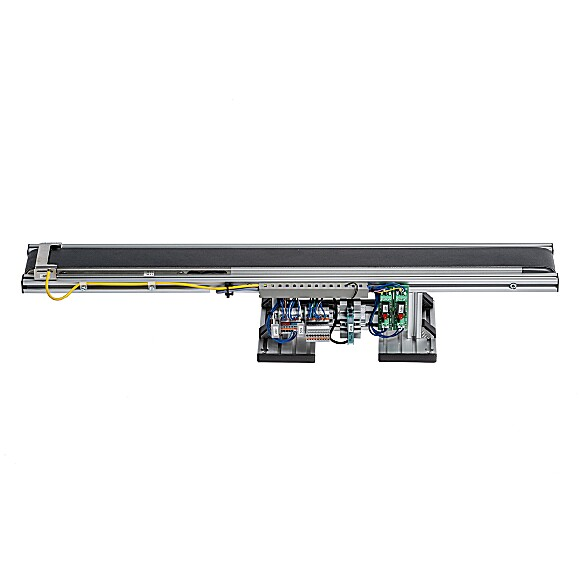
\includegraphics[trim={0 6cm 0 5cm},clip,width=8cm]{maquete/esteira/40778_3.jpg}
    };
    % \draw[red,ultra thick,rounded corners] (0,0) rectangle (9.4,6.2);
    \begin{scope}[x={(image.south east)},y={(image.north west)}]
        % \draw[help lines,xstep=.1,ystep=.1] (0,0) grid (1,1);
        % \foreach \x in {0,1,...,9} { \node [anchor=north] at (\x/10,0) {0.\x}; }
        % \foreach \y in {0,1,...,9} { \node [anchor=east] at (0,\y/10) {0.\y}; }
        \draw [->,>=stealth,red, very thick](0.9,0.7) -- (0.1,0.7);
        \draw [red] (0.5,0.8) node {Forward};
        \draw [->,>=stealth,red, very thick](0.1,0.1) -- (0.9,0.1);
        \draw [red](0.5,0.0) node {Reverse};
      \end{scope}
  \end{tikzpicture}
  \caption{Conveyor Belt}
\end{figure}

\begin{figure}[H]
  \centering
  \begin{tikzpicture}
    \node[anchor=south west,inner sep=0] (image) at (0,0) {
      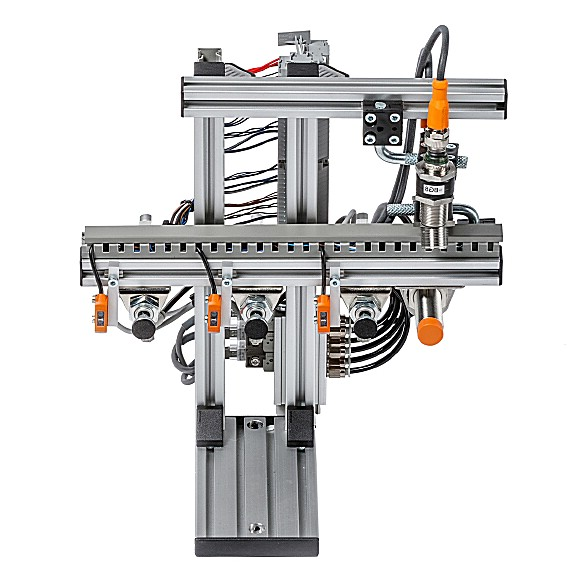
\includegraphics[trim={0 0 0 0},clip,width=8cm]{maquete/sensores/69511_3.jpg}
    };
    % \draw[red,ultra thick,rounded corners] (0,0) rectangle (9.4,6.2);
    \begin{scope}[x={(image.south east)},y={(image.north west)}]
        % \draw[help lines,xstep=.1,ystep=.1] (0,0) grid (1,1);
        % \foreach \x in {0,1,...,9} { \node [anchor=north] at (\x/10,0) {0.\x}; }
        % \foreach \y in {0,1,...,9} { \node [anchor=east] at (0,\y/10) {0.\y};  }
        \draw[red,ultra thick,rounded corners] (0.15,0.4) rectangle ++ (0.15,0.1);
        \draw[red] (0.1,0.1) node {\textbf{Left}};
        \draw[->,>=stealth,red, very thick] (0.2,0.38) -- (0.1,0.15);
        \draw[magenta,ultra thick,rounded corners] (0.35,0.4) rectangle ++ (0.15,0.1);
        \draw[magenta] (0.1,0.8) node {\textbf{Center}};
        \draw[->,>=stealth,magenta, very thick] (0.4,0.52) -- (0.2,0.75);
        \draw[cyan,ultra thick,rounded corners] (0.53,0.4) rectangle ++ (0.15,0.1);
        \draw[cyan] (0.7,0.1) node {\textbf{Right}};
        \draw[->,>=stealth,cyan, very thick] (0.65,0.38) -- (0.7,0.15);
      \end{scope}
  \end{tikzpicture}
  \caption{Sensors}
\end{figure}

\begin{figure}[H]
  \centering
  \begin{tikzpicture}
    \node[anchor=south west,inner sep=0] (image) at (0,0) {
      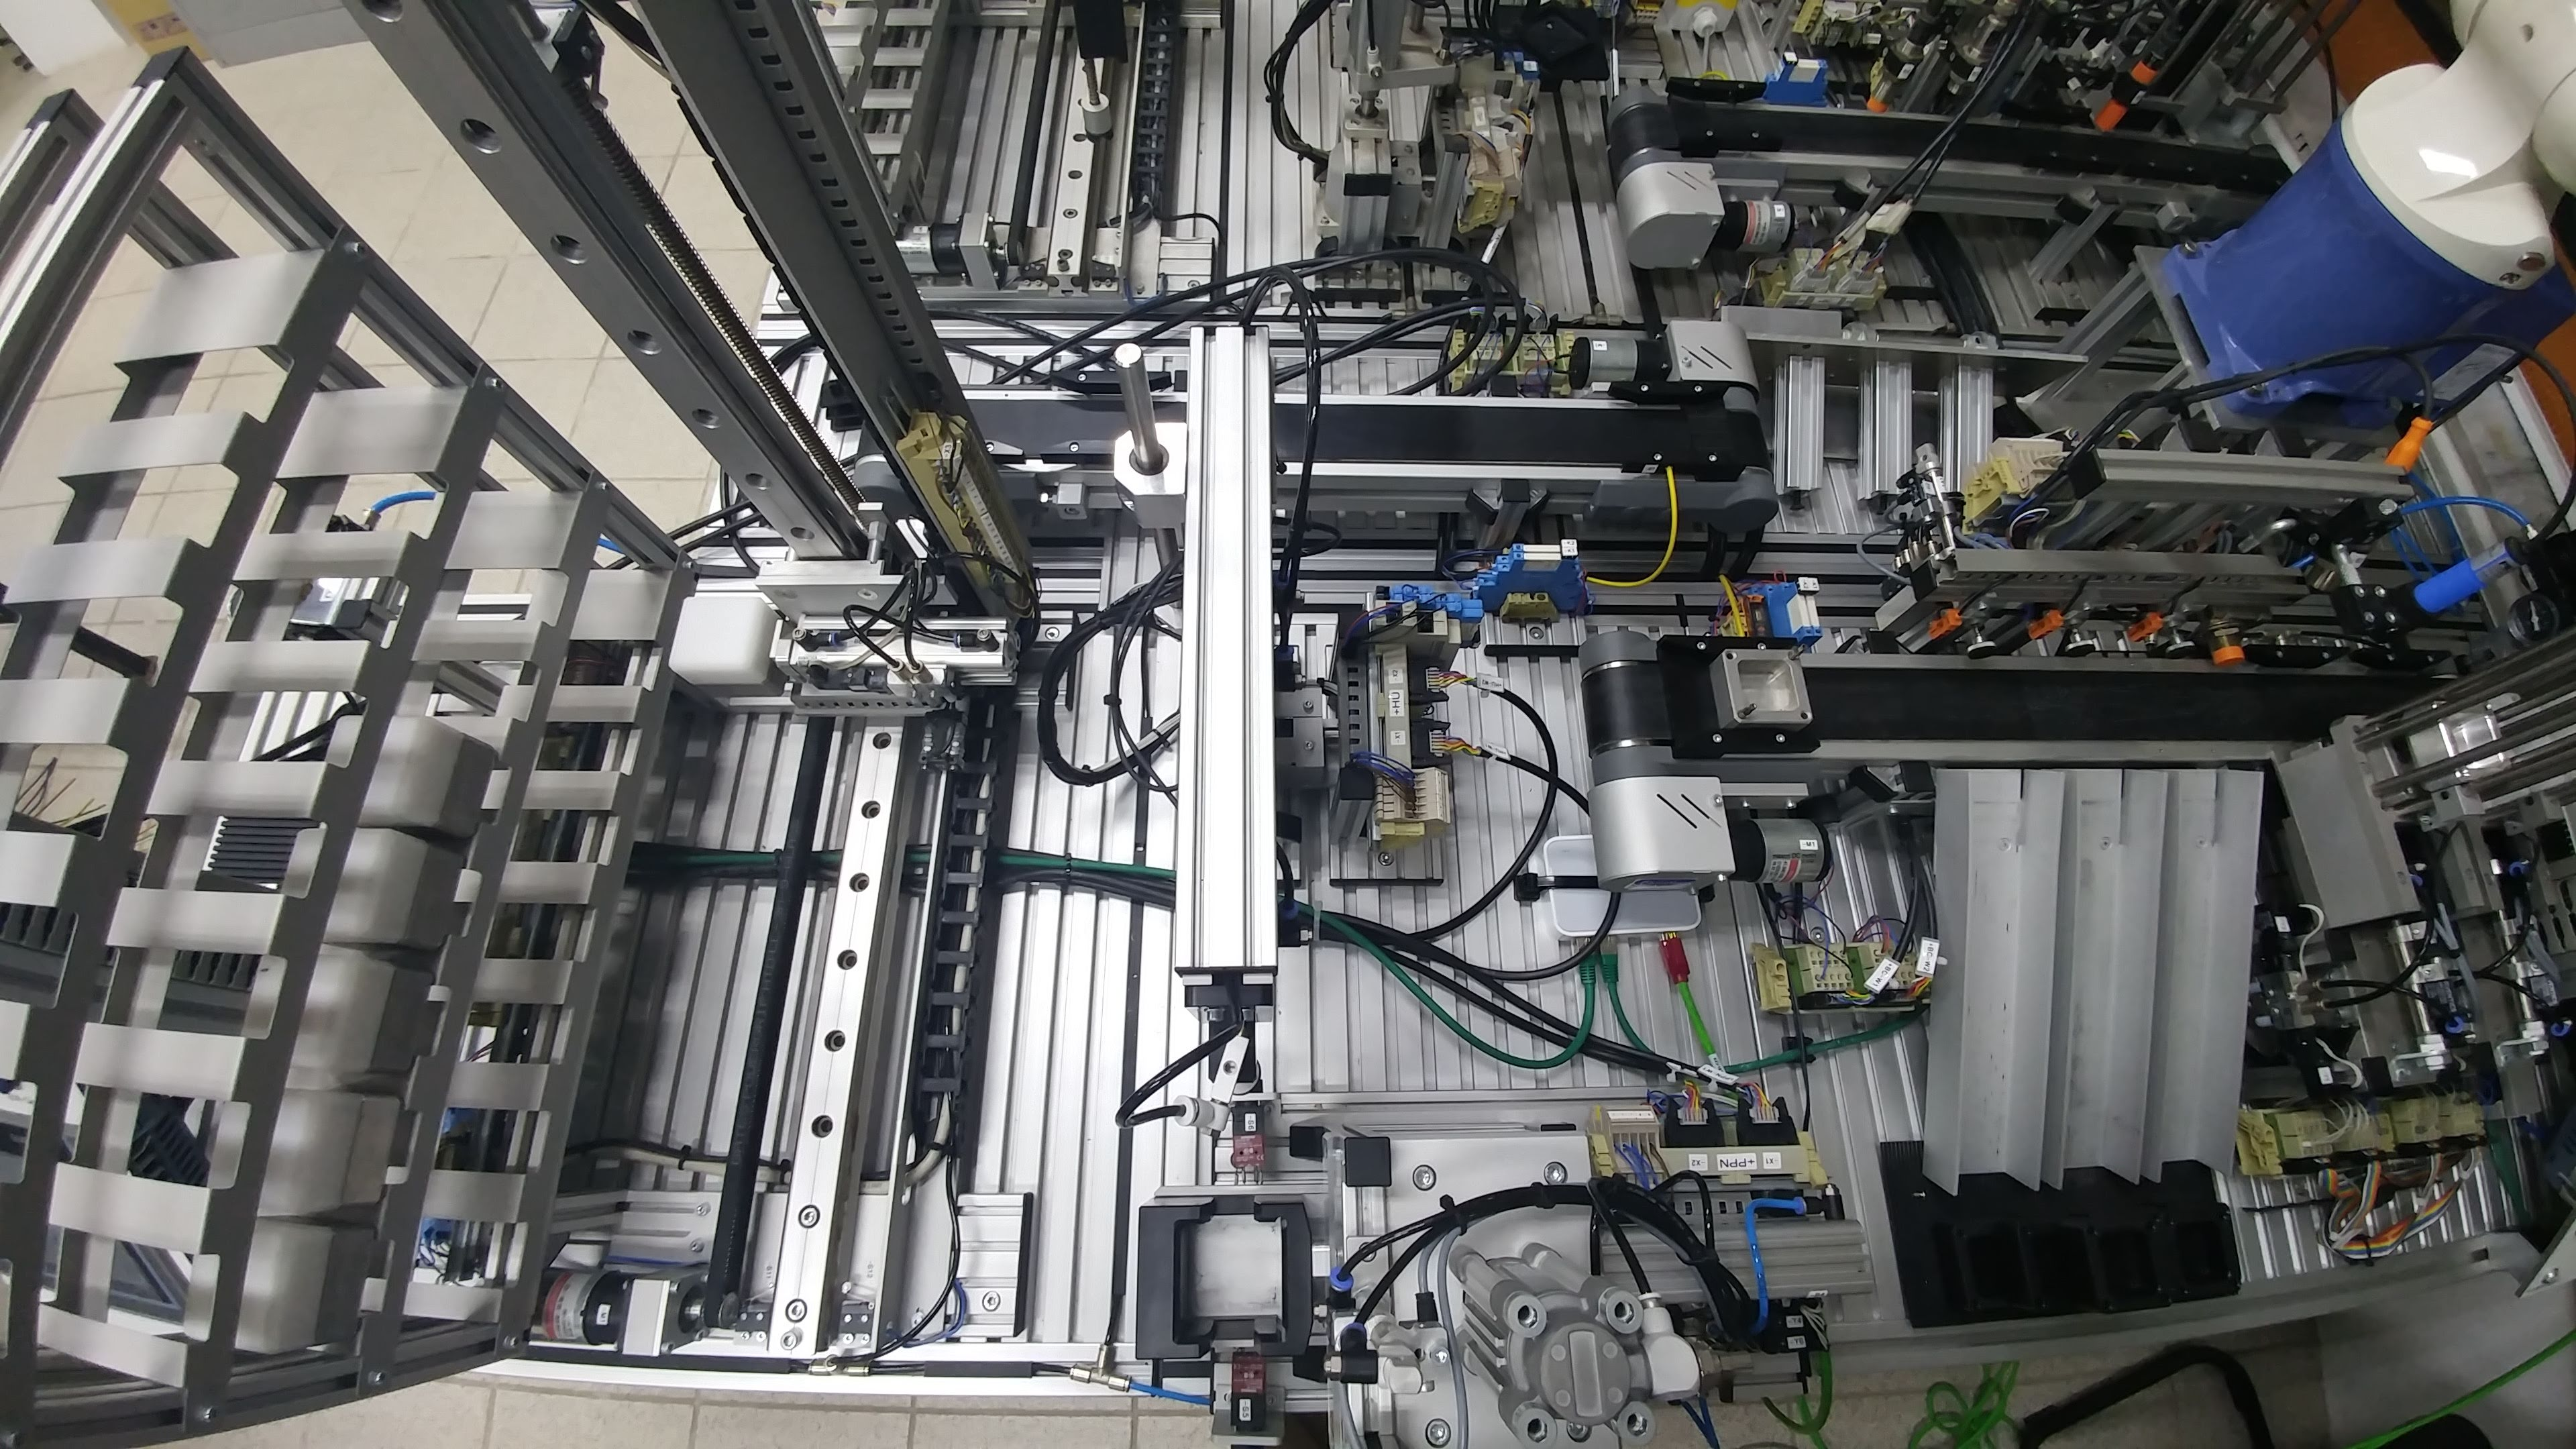
\includegraphics[trim={20cm 0 30cm 20cm},clip,width=0.8\textwidth]{maquete/armAngles.jpg}
    };
    % \draw[red,ultra thick,rounded corners] (0,0) rectangle (9.4,6.2);
    \begin{scope}[x={(image.south east)},y={(image.north west)}]
        % \draw[help lines,xstep=.1,ystep=.1] (0,0) grid (1,1);
        % \foreach \x in {0,1,...,9} { \node [anchor=north] at (\x/10,0) {0.\x}; }
        % \foreach \y in {0,1,...,9} { \node [anchor=east] at (0,\y/10) {0.\y}; }a
        
      
        \draw[red,->,>=stealth,very thick] (0.48,0.9) -- ++(-50:0.7);
        \draw[red,->,>=stealth,very thick] (0.48,0.9) -- ++(-95:0.7);
        \draw[red,->,>=stealth,very thick] (0.48,0.9) -- ++(-120:0.7);

        \draw[fill=red, fill opacity=0.2,draw=none] (0.48,0.9) -- ([shift=(-50:0.5)]0.48,0.9) arc (-50:-95:0.5);
        \draw[fill=blue, fill opacity=0.2,draw=none] (0.48,0.9) -- ([shift=(-95:0.5)]0.48,0.9) arc (-95:-120:0.5);

        \draw [fill,white,fill opacity=0.7,draw=none] (0.02,0.23) rectangle ++ (0.35,0.06);
        \draw [black] (0.2,0.25) node {\tiny \textbf{STORAGE\_ANGLE\_BEFORE}};

        \draw [fill,white,fill opacity=0.7,draw=none] (0.25,0.13) rectangle ++ (0.3,0.06);
        \draw [black] (0.4,0.15) node {\tiny \textbf{PRESS\_ANGLE\_AFTER}};

        \draw [fill,white,fill opacity=0.7,draw=none] (0.7,0.28) rectangle ++ (0.3,0.06);
        \draw [black] (0.85,0.3) node {\tiny \textbf{PRESS\_ANGLE\_BEFORE}};

        \draw [fill,white,fill opacity=0.7,draw=none] (0.1,0.82) rectangle  (0.2,0.96);
        \draw [red,thick] ([shift=(0:0.03)]0.15,0.9) arc (0:180:0.03);
        \draw[black,->,>=stealth,very thick] (0.15,0.85) -- ++(0,0.1);
        \draw [red,->,>=stealth,thick] ([shift=(0:-0.03)]0.15,0.9) arc (-180:-20:0.03);

      \end{scope}
  \end{tikzpicture}
  \caption{Sensors}
\end{figure}

Identification algorithm as seen in \cite{moreira2018enhanced}
\begin{algorithm2e}
  \caption{Identification Algorithm}\label{alg:identification}
\KwIn
{%
Modified observed paths $p_i^k$, for i= 1,\dots,$r$
}
\KwOut
{%
DAOCT = $($\XSet,\SigmaSet,\OmegaSet,\ffunction,\lambdafunction,\RSet,\thetafunction,\xZero,\XfSet$)$
}
\BlankLine
Create an initial state $x_0$, and define $\lambda(x_0) = \tilde{\lambda}(x_0) =
y_{1,1}$

$X = \{ x_0\}, X_f = \emptyset$

\For{$i = 1$ \KwTo $r$}
{
\For{$j = 1$ \KwTo $l_i - 1$}
{
  Find the State $x \in X $ such that $\tilde{\lambda}(x) = y_{i,j+1}$

  \eIf{$\tilde{\lambda}(x) \neq y_{i,j+1}$ for all $ x \in X$}
  { Create state $x^\prime$ and define $\tilde{\lambda}(x^\prime) = y_{i,j+1}$

$X = X \cup \{ x^\prime\}$

$\lambda(x^\prime) = \tilde{\lambda_l}(x^\prime)$

}
{
  Find $x^\prime \in X$ such that $\tilde{\lambda}(x^\prime) = y_{i,j+1}$
}
$f(x,\sigma_{i,j}) = x^\prime$

Add $i$ to $\theta(x,\sigma_{i,j})$

\If{$j = l_i - 1$}
{
  $X_f = X_f \cup \{x^\prime\}$
}
}
}
\end{algorithm2e}

% \begin{table}[H]
%   \centering
%   \caption{table}
%   \begin{tabular}{cc}
%     \label{tab:tab1}
%     \hypertarget{tab:1}{}
%     Transição&Significado\\
%     \hline \\
%     \hyperlink{partialNet:t1}{\hypertarget{partialTable:t1}{$t_{1}$}}&Test\\
%     \hyperlink{partialNet:p1}{\hypertarget{partialTable:p1}{$p_{1}$}}&balbalbal\\
%     \hyperlink{partialNet:p0m2}{\hypertarget{partialTable:p0m2}{$p_{0}$}}&balbalbal
%   \end{tabular}
% \end{table}

% \newpage
% \begin{figure}[h]
%   \centering
%   \begin{tikzpicture}[>=latex',line join=bevel,]
%%
\node (p0m2) at (27.0bp,18.0bp) [draw,ellipse,place, tokens=2, label=above:, label=left:\hyperlink{partialTable:p0m2}{\hypertarget{partialNet:p0m2}{$p_{0}$}},rotate=90] {};
  \node (tt1) at (114.0bp,18.0bp) [draw,ellipse,timedtransition, label=above:, label=left:\hyperlink{partialTable:tt1}{\hypertarget{partialNet:tt1}{$t_{1}$}},rotate=90] {};
  \node (ep1) at (185.0bp,18.0bp) [draw,ellipse,extPlace, label=above:, label=left:\hyperlink{partialNet:p1}{$p_{1}$},rotate=90] {};
  \draw [-Latex,inhibitor] (p0m2) ..controls (54.05bp,18.0bp) and (76.966bp,18.0bp)  .. (tt1);
  \definecolor{strokecol}{rgb}{0.0,0.0,0.0};
  \pgfsetstrokecolor{strokecol}
  \draw (70.5bp,27.0bp) node {3};
  \draw [-Latex] (tt1) ..controls (141.25bp,18.0bp) and (147.94bp,18.0bp)  .. (ep1);
%
\end{tikzpicture}

%   \caption{example }
%   \label{fig:example}
% \end{figure}

% \newpage
% \begin{figure}[h]
%   \centering
%   \begin{tikzpicture}[>=latex',line join=bevel,]
%%
\node (et1) at (27.0bp,18.0bp) [draw,ellipse,extTransition, label=above:, label=left:\hyperlink{partialNet:t1}{$t_{1}$},rotate=90] {};
  \node (p1) at (95.0bp,18.0bp) [draw,ellipse,place, label=above:, label=left:\hyperlink{partialTable:p1}{\hypertarget{partialNet:p1}{$p_{1}$}},rotate=90] {};
  \draw [-Latex] (et1) ..controls (54.266bp,18.0bp) and (57.727bp,18.0bp)  .. (p1);
%
\end{tikzpicture}

%   \caption{example }
%   \label{fig:example}
% \end{figure}

% \newpage

% \begin{figure}[H]
%   \centering
%   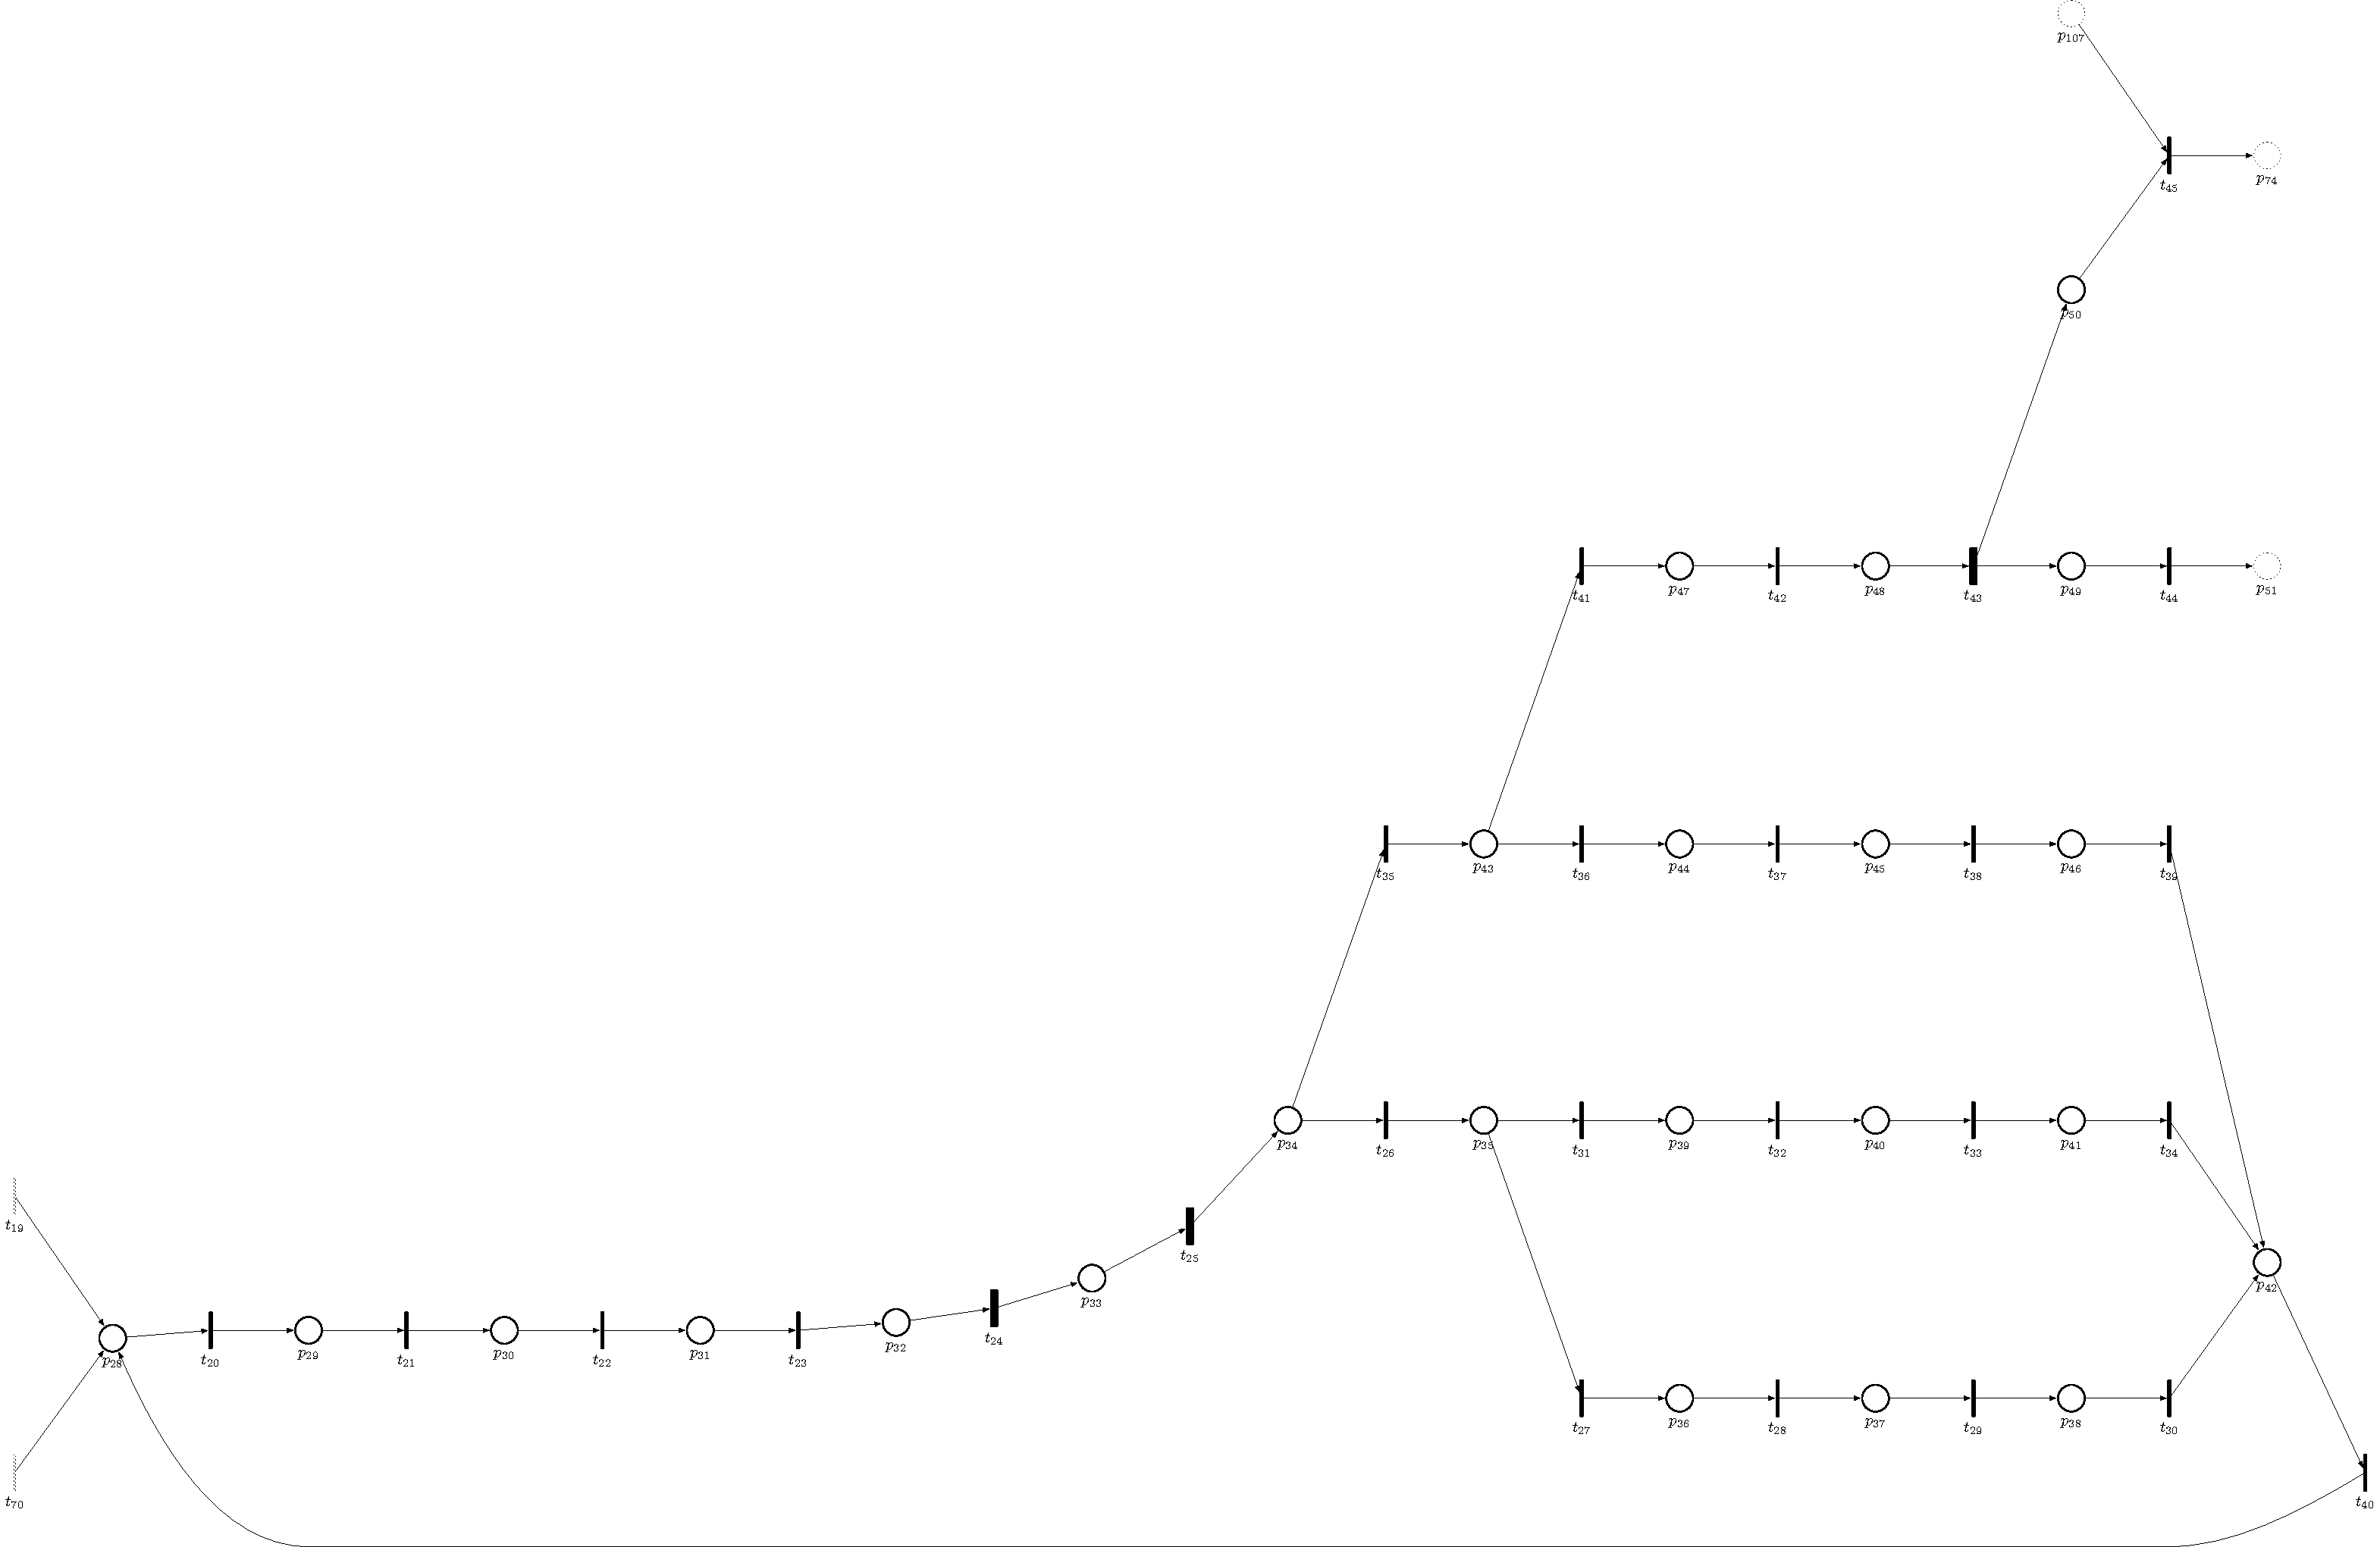
\includegraphics{../../figures/petriNet/dot/2-metalv/metalv.pdf}
%   \caption{qlksdjf}
%   \label{fig:example}
% \end{figure}


% \begin{figure}[H]
%   \centering
%   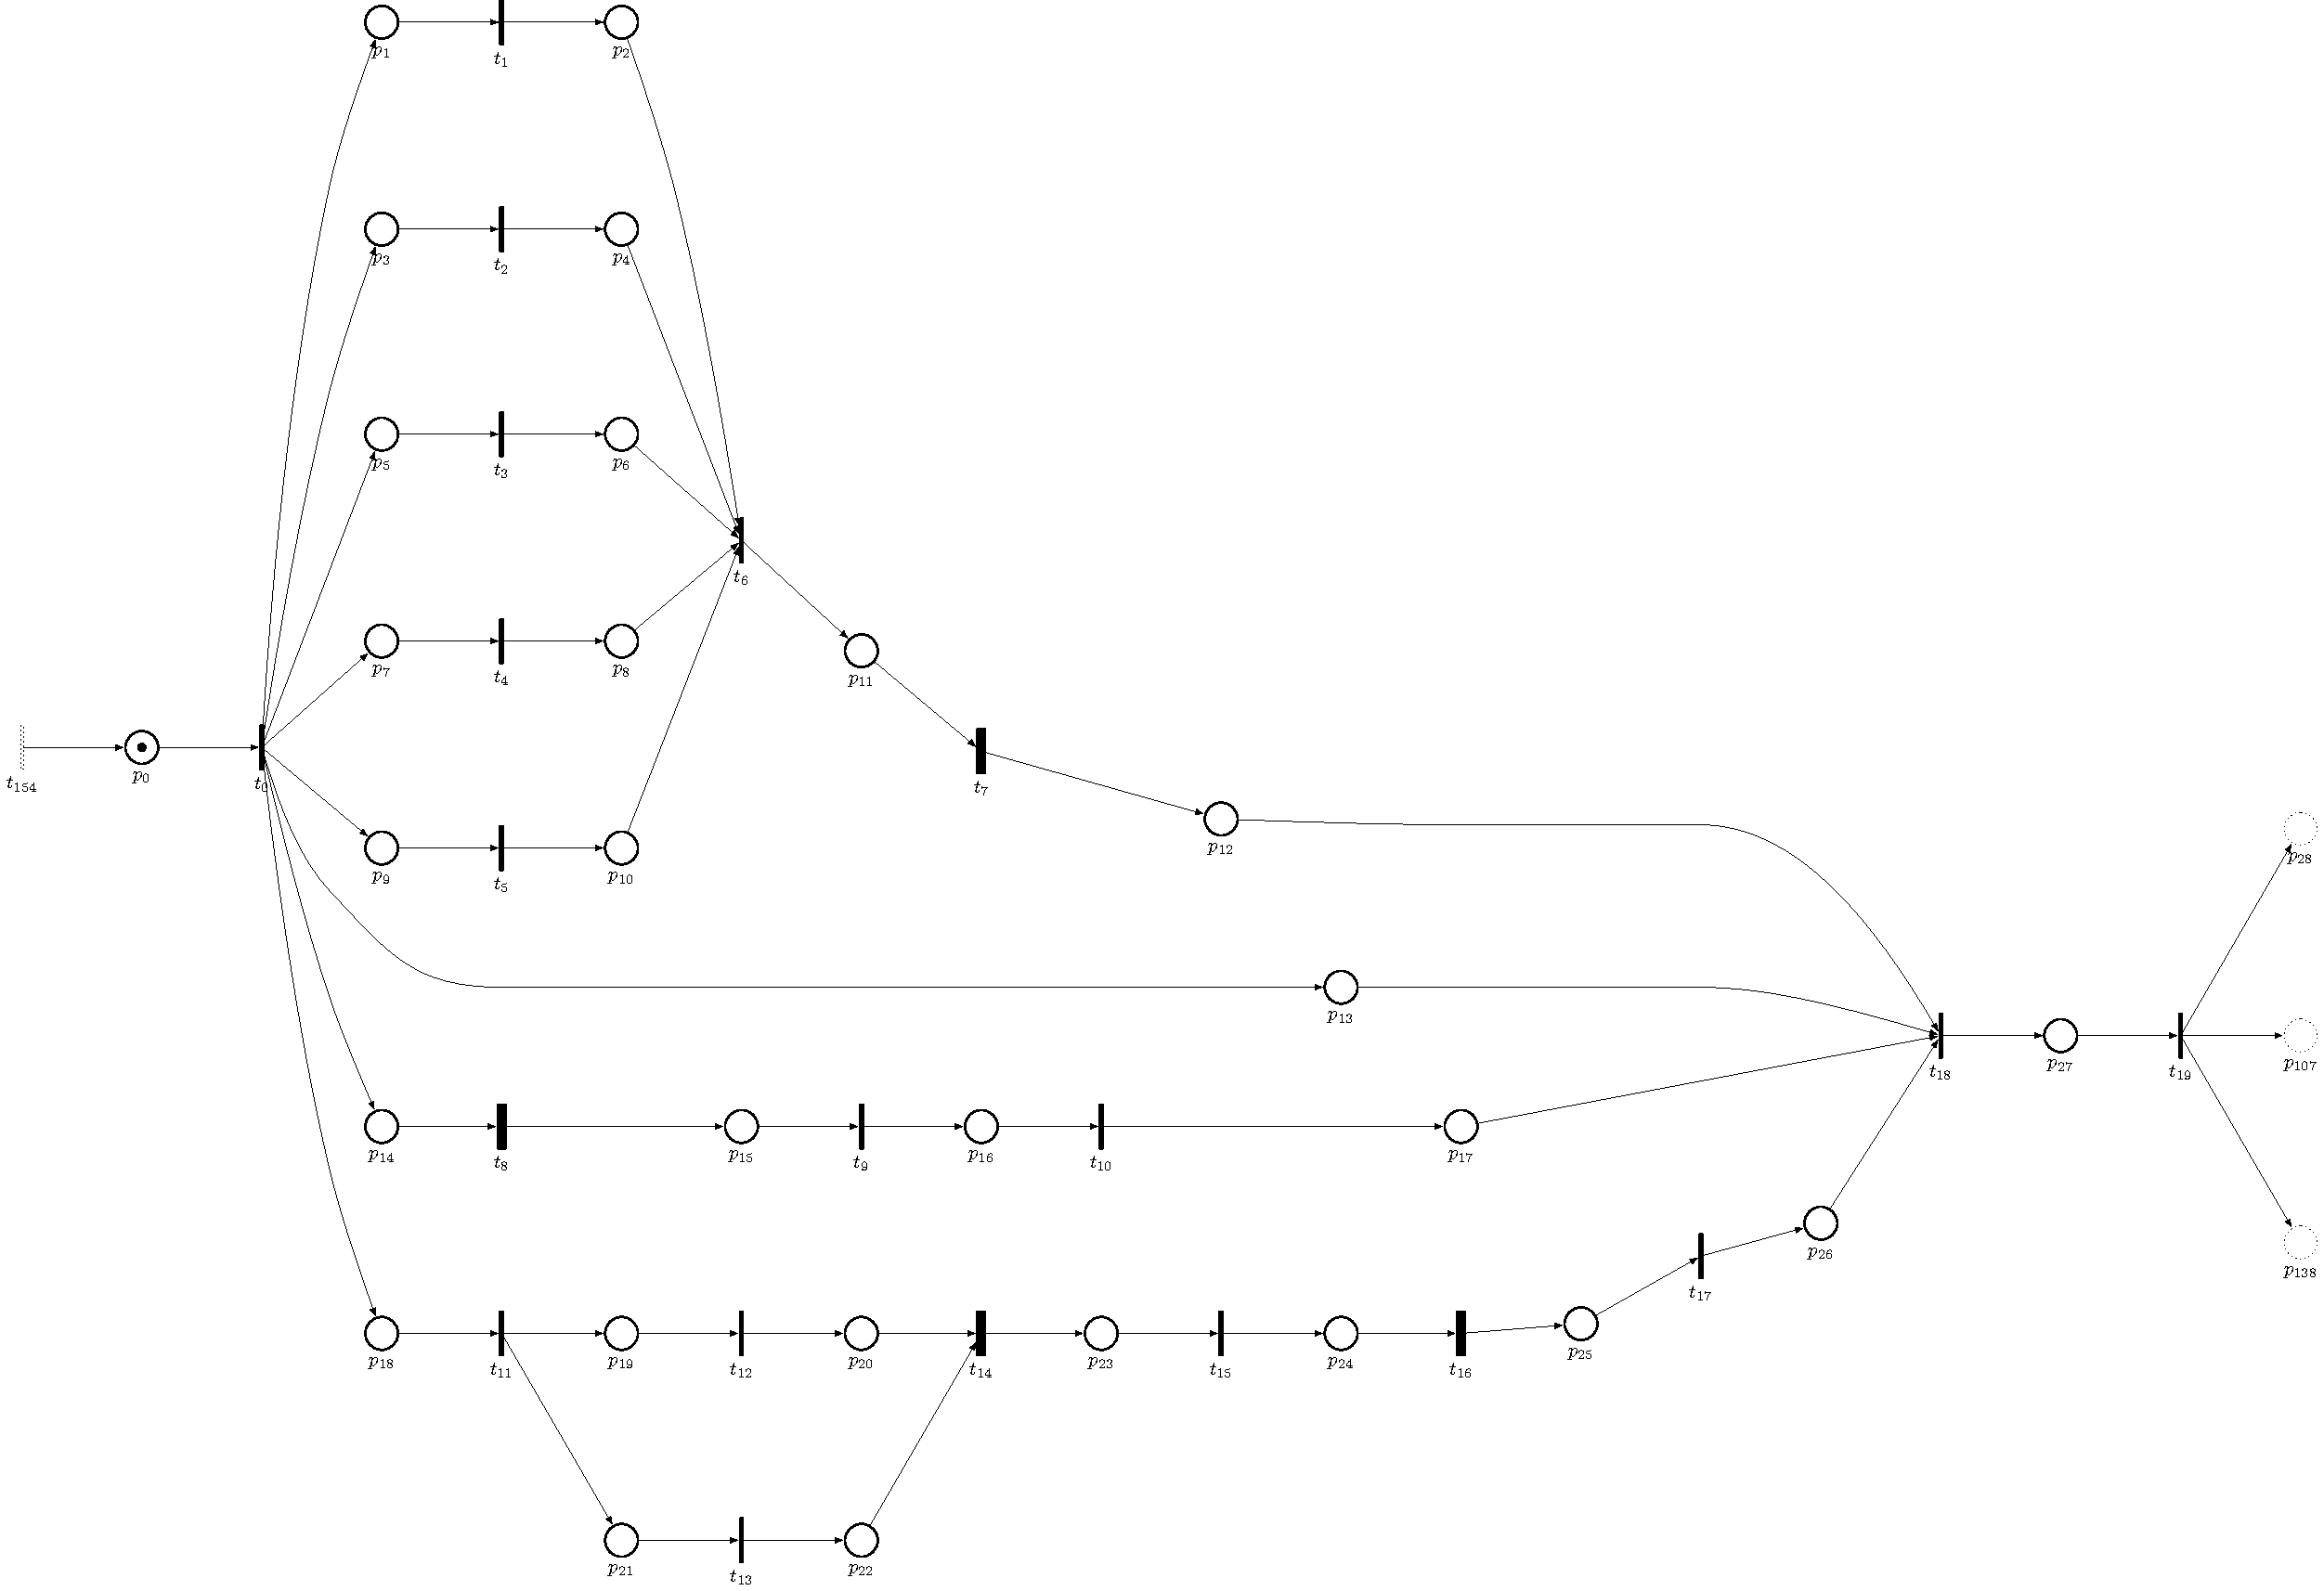
\includegraphics[width=0.4\textwidth]{../../figures/partial/initial.tikz}
%   \caption{petri net bal}
%   \label{fig:petrinetexample}
% \end{figure}

% \addtikzfigure{../../figures/petriNet/partial/initial}
% {Petri net of cube storage module.}
% {petri_initialization}

% \addtikzfigure{../../figures/petriNet//partial/metalv}
% {Petri net of metal cube half sorting module.}
% {petri_initialization}

\begin{table}[htbp]
\caption{Initialization Module Places.}
\centering
\begin{tabular}{M{5cm}M{10cm}}
Places & Meaning\\
\hline
\hyperlink{partialNet:p0m1}{\hypertarget{partialTable:p0m1}{$p_{0}$}} & System Stopped\\
\hyperlink{partialNet:p1}{\hypertarget{partialTable:p1}{$p_{1}$}} & Retract MAG1's Cylinder *\\
\hyperlink{partialNet:p2}{\hypertarget{partialTable:p2}{$p_{2}$}} & MAG1's Cylinder Retracted\\
\hyperlink{partialNet:p3}{\hypertarget{partialTable:p3}{$p_{3}$}} & Retract MAG2's Cylinder *\\
\hyperlink{partialNet:p4}{\hypertarget{partialTable:p4}{$p_{4}$}} & MAG2's Cylinder Retracted\\
\hyperlink{partialNet:p5}{\hypertarget{partialTable:p5}{$p_{5}$}} & Retract Right Discharge Cylinder *\\
\hyperlink{partialNet:p6}{\hypertarget{partialTable:p6}{$p_{6}$}} & Right Discharge Cylinder Retracted\\
\hyperlink{partialNet:p7}{\hypertarget{partialTable:p7}{$p_{7}$}} & Retract Center Discharge Cylinder\\
\hyperlink{partialNet:p8}{\hypertarget{partialTable:p8}{$p_{8}$}} & Center Discharge Cylinder Retracted\\
\hyperlink{partialNet:p9}{\hypertarget{partialTable:p9}{$p_{9}$}} & Retract Left Discharge Cylinder *\\
\hyperlink{partialNet:p10}{\hypertarget{partialTable:p10}{$p_{10}$}} & Left Discharge Cylinder Retracted\\
\hyperlink{partialNet:p11}{\hypertarget{partialTable:p11}{$p_{11}$}} & Turn Conveyor Belt On (Reverse)\\
\hyperlink{partialNet:p12}{\hypertarget{partialTable:p12}{$p_{12}$}} & No Pieces On Conveyor Belt\\
\hyperlink{partialNet:p13}{\hypertarget{partialTable:p13}{$p_{13}$}} & Reset Variables\\
\hyperlink{partialNet:p14}{\hypertarget{partialTable:p14}{$p_{14}$}} & Raise Press\\
\hyperlink{partialNet:p15}{\hypertarget{partialTable:p15}{$p_{15}$}} & Open Safety Door\\
\hyperlink{partialNet:p16}{\hypertarget{partialTable:p16}{$p_{16}$}} & Extend Assembly Unit Holder\\
\hyperlink{partialNet:p17}{\hypertarget{partialTable:p17}{$p_{17}$}} & Assembly Unit Ready\\
\hyperlink{partialNet:p18}{\hypertarget{partialTable:p18}{$p_{18}$}} & Arm Lowered and Retracted, and Storage Unit Retracted\\
\hyperlink{partialNet:p19}{\hypertarget{partialTable:p19}{$p_{19}$}} & Move Storage Unit to the Right\\
\hyperlink{partialNet:p20}{\hypertarget{partialTable:p20}{$p_{20}$}} & Storage Unit ready ( horizontal )\\
\hyperlink{partialNet:p21}{\hypertarget{partialTable:p21}{$p_{21}$}} & Move Storage Device Downwards\\
\hyperlink{partialNet:p22}{\hypertarget{partialTable:p22}{$p_{22}$}} & Storage Unit ready ( vertical )\\
\hyperlink{partialNet:p23}{\hypertarget{partialTable:p23}{$p_{23}$}} & Rotate Arm CCW\\
\hyperlink{partialNet:p24}{\hypertarget{partialTable:p24}{$p_{24}$}} & Turn HSC Off ( Arm Stopped )\\
\hyperlink{partialNet:p25}{\hypertarget{partialTable:p25}{$p_{25}$}} & Rotate Arm CW\\
\hyperlink{partialNet:p26}{\hypertarget{partialTable:p26}{$p_{26}$}} & Arm Stopped facing conveyor belt\\
\hyperlink{partialNet:p27}{\hypertarget{partialTable:p27}{$p_{27}$}} & System Ready\\
\end{tabular}
\end{table}


\begin{table}[H]
\caption{Initialization Module Transitions.}
\centering
\begin{tabular}{M{5cm}M{10cm}}
Transitions & Meaning\\
\hline
\hyperlink{partialNet:t0}{\hypertarget{partialTable:t0}{$t_{0}$}} & Initialization Button\\
\hyperlink{partialNet:t1}{\hypertarget{partialTable:t1}{$t_{1}$}} & MAG1's Cylinder Retracted\\
\hyperlink{partialNet:t2}{\hypertarget{partialTable:t2}{$t_{2}$}} & MAG2's Cylinder Retracted\\
\hyperlink{partialNet:t3}{\hypertarget{partialTable:t3}{$t_{3}$}} & Right Discharge Cylinder Retracted\\
\hyperlink{partialNet:t4}{\hypertarget{partialTable:t4}{$t_{4}$}} & Center Discharge Cylinder Retracted\\
\hyperlink{partialNet:t5}{\hypertarget{partialTable:t5}{$t_{5}$}} & Left Discharge Cylinder Retracted\\
\hyperlink{partialNet:t6}{\hypertarget{partialTable:t6}{$t_{6}$}} & \\
\hyperlink{partialNet:tt7}{\hypertarget{partialTable:tt7}{$t_{7}$}} & T=12s\\
\hyperlink{partialNet:tt8}{\hypertarget{partialTable:tt8}{$t_{8}$}} & T=2.5s\\
\hyperlink{partialNet:t9}{\hypertarget{partialTable:t9}{$t_{9}$}} & Safety Door Opened\\
\hyperlink{partialNet:t10}{\hypertarget{partialTable:t10}{$t_{10}$}} & Assembly Unit Holder Extended\\
\hyperlink{partialNet:t11}{\hypertarget{partialTable:t11}{$t_{11}$}} & Storage Unit Retracted and Arm Lowered and Retracted\\
\hyperlink{partialNet:t12}{\hypertarget{partialTable:t12}{$t_{12}$}} & Storage Unit Right Limit Switch\\
\hyperlink{partialNet:t13}{\hypertarget{partialTable:t13}{$t_{13}$}} & Storage Unit Inferior Limit Switch\\
\hyperlink{partialNet:tt14}{\hypertarget{partialTable:tt14}{$t_{14}$}} & T=2s\\
\hyperlink{partialNet:t15}{\hypertarget{partialTable:t15}{$t_{15}$}} & Inductive Sensor Arm\\
\hyperlink{partialNet:tt16}{\hypertarget{partialTable:tt16}{$t_{16}$}} & T=1s\\
\hyperlink{partialNet:t17}{\hypertarget{partialTable:t17}{$t_{17}$}} & ARMCOUNTER <= BELT\_ANGLE\_CW\\
\hyperlink{partialNet:t18}{\hypertarget{partialTable:t18}{$t_{18}$}} & \\
\hyperlink{partialNet:t19}{\hypertarget{partialTable:t19}{$t_{19}$}} & Start Button\\
\end{tabular}
\end{table}


\begin{longtable}{M{5cm}M{10cm}}
\caption{Metal Half-cube Selection Module Places.} \label{tab:metalvPlaces}
\\
Places & Meaning\\
\hline
\endfirsthead
\multicolumn{2}{l}{Continued from previous page} \\
\hline

Places & Meaning \\

\hline
\endhead
\hline\multicolumn{2}{r}{Continued on next page} \\
\endfoot
\endlastfoot
\hline
\hyperlink{partialNet:p28}{\hypertarget{partialTable:p28}{$p_{28}$}} & MAG1 Empty\\
\hyperlink{partialNet:p29}{\hypertarget{partialTable:p29}{$p_{29}$}} & MAG1 Not Empty\\
\hyperlink{partialNet:p30}{\hypertarget{partialTable:p30}{$p_{30}$}} & Extend MAG1's Cylinder *\\
\hyperlink{partialNet:p31}{\hypertarget{partialTable:p31}{$p_{31}$}} & Retract MAG1's Cylinder *\\
\hyperlink{partialNet:p32}{\hypertarget{partialTable:p32}{$p_{32}$}} & MAG1's Cylinder Retracted\\
\hyperlink{partialNet:p33}{\hypertarget{partialTable:p33}{$p_{33}$}} & Turn Conveyor Belt On\\
\hyperlink{partialNet:p34}{\hypertarget{partialTable:p34}{$p_{34}$}} & \\
\hyperlink{partialNet:p35}{\hypertarget{partialTable:p35}{$p_{35}$}} & Plastic Half-cube\\
\hyperlink{partialNet:p36}{\hypertarget{partialTable:p36}{$p_{36}$}} & Turn Conveyor Belt On\\
\hyperlink{partialNet:p37}{\hypertarget{partialTable:p37}{$p_{37}$}} & Extend Right Discharge Cylinder *\\
\hyperlink{partialNet:p38}{\hypertarget{partialTable:p38}{$p_{38}$}} & Retract Right Discharge Cylinder *\\
\hyperlink{partialNet:p39}{\hypertarget{partialTable:p39}{$p_{39}$}} & Turn Conveyor Belt On\\
\hyperlink{partialNet:p40}{\hypertarget{partialTable:p40}{$p_{40}$}} & Extend Center Discharge Cylinder *\\
\hyperlink{partialNet:p41}{\hypertarget{partialTable:p41}{$p_{41}$}} & Retract Center Discharge Cylinder *\\
\hyperlink{partialNet:p42}{\hypertarget{partialTable:p42}{$p_{42}$}} & \\
\hyperlink{partialNet:p43}{\hypertarget{partialTable:p43}{$p_{43}$}} & Metal Half-cube\\
\hyperlink{partialNet:p44}{\hypertarget{partialTable:p44}{$p_{44}$}} & Turn Conveyor Belt On\\
\hyperlink{partialNet:p45}{\hypertarget{partialTable:p45}{$p_{45}$}} & Extend Left Discharge Cylinder *\\
\hyperlink{partialNet:p46}{\hypertarget{partialTable:p46}{$p_{46}$}} & Retract Left Discharge Cylinder *\\
\hyperlink{partialNet:p47}{\hypertarget{partialTable:p47}{$p_{47}$}} & Turn Conveyor Belt On\\
\hyperlink{partialNet:p48}{\hypertarget{partialTable:p48}{$p_{48}$}} & Turn Conveyor Belt On\\
\hyperlink{partialNet:p49}{\hypertarget{partialTable:p49}{$p_{49}$}} & Metal Half-cube Ready\\
\hyperlink{partialNet:p50}{\hypertarget{partialTable:p50}{$p_{50}$}} & Conveyor Belt Stopped\\
\end{longtable}


\begin{table}[H]
\caption{Metal Half-cube Selection Module Transitions.}
\centering
\begin{tabular}{M{5cm}M{10cm}}
Transitions & Meaning\\
\hline
\hyperlink{partialNet:t20}{\hypertarget{partialTable:t20}{$t_{20}$}} & \(\overline{\mbox{MAG1 Empty}}\)\\
\hyperlink{partialNet:t21}{\hypertarget{partialTable:t21}{$t_{21}$}} & \\
\hyperlink{partialNet:t22}{\hypertarget{partialTable:t22}{$t_{22}$}} & MAG1's Cylinder Extended \(\uparrow\)\\
\hyperlink{partialNet:t23}{\hypertarget{partialTable:t23}{$t_{23}$}} & MAG1's Cylinder Retracted \(\uparrow\)\\
\hyperlink{partialNet:tt24}{\hypertarget{partialTable:tt24}{$t_{24}$}} & T=0.5s\\
\hyperlink{partialNet:tt25}{\hypertarget{partialTable:tt25}{$t_{25}$}} & Presence \(\uparrow\) T=0.5s\\
\hyperlink{partialNet:t26}{\hypertarget{partialTable:t26}{$t_{26}$}} & \(\overline{\mbox{Metallic Sensor}}\)\\
\hyperlink{partialNet:t27}{\hypertarget{partialTable:t27}{$t_{27}$}} & \(\overline{\mbox{White Color Sensor}}\)\\
\hyperlink{partialNet:t28}{\hypertarget{partialTable:t28}{$t_{28}$}} & Proximity Sensor Left Discharge Cylinder \(\uparrow\)\\
\hyperlink{partialNet:t29}{\hypertarget{partialTable:t29}{$t_{29}$}} & Right Discharge Cylinder Extended\\
\hyperlink{partialNet:t30}{\hypertarget{partialTable:t30}{$t_{30}$}} & Right Discharge Cylinder Retracted\\
\hyperlink{partialNet:t31}{\hypertarget{partialTable:t31}{$t_{31}$}} & White Color Sensor\\
\hyperlink{partialNet:t32}{\hypertarget{partialTable:t32}{$t_{32}$}} & Proximity Sensor Center Discharge Cylinder \(\uparrow\)\\
\hyperlink{partialNet:t33}{\hypertarget{partialTable:t33}{$t_{33}$}} & Center Discharge Cylinder Extended\\
\hyperlink{partialNet:t34}{\hypertarget{partialTable:t34}{$t_{34}$}} & Center Discharge Cylinder Retracted\\
\hyperlink{partialNet:t35}{\hypertarget{partialTable:t35}{$t_{35}$}} & Metallic Sensor\\
\hyperlink{partialNet:t36}{\hypertarget{partialTable:t36}{$t_{36}$}} & Concavity Downwards\\
\hyperlink{partialNet:t37}{\hypertarget{partialTable:t37}{$t_{37}$}} & Proximity Sensor Left Discharge Cylinder \(\uparrow\)\\
\hyperlink{partialNet:t38}{\hypertarget{partialTable:t38}{$t_{38}$}} & Left Discharge Cylinder Extended\\
\hyperlink{partialNet:t39}{\hypertarget{partialTable:t39}{$t_{39}$}} & Left Discharge Cylinder Retracted\\
\hyperlink{partialNet:t40}{\hypertarget{partialTable:t40}{$t_{40}$}} & \\
\hyperlink{partialNet:t41}{\hypertarget{partialTable:t41}{$t_{41}$}} & Concavity Upwards\\
\hyperlink{partialNet:t42}{\hypertarget{partialTable:t42}{$t_{42}$}} & Proximity Sensor End Of Conveyor Belt \(\uparrow\)\\
\hyperlink{partialNet:tt43}{\hypertarget{partialTable:tt43}{$t_{43}$}} & T=0.5s\\
\hyperlink{partialNet:t44}{\hypertarget{partialTable:t44}{$t_{44}$}} & Proximity Sensor End Of Conveyor Belt \(\downarrow\)\\
\hyperlink{partialNet:t45}{\hypertarget{partialTable:t45}{$t_{45}$}} & \\
\end{tabular}
\end{table}


%%% Local Variables:
%%% mode: latex
%%% TeX-master: "../monografia"
%%% End:



\chapter{Introduction}
In a world where the majority of the population lives in industrial societies,
and machines take part on the bulk of the production of almost all goods: from
food to cosmetics and drugs, from toothbrushes to automobiles, 
a well-paced throughput it is crucial, and any non expected halt on the
production or change can be disastrous, producing sometimes multimillionaire debts,
provoking a snowball effect, affecting the economy and consequentially the welfare of the society.

A diverse number of causes of the halt or change of the throughput can be
accounted for. Some are as simple as a power outage, or a component malfunction,
but nowadays there are other players. As the industry \textsl{walks}, or even
better \textsl{runs}, towards the so called Fourth Industrial Revolution, the industry
urges the use of \textit{connected sensors}, since the Internet of Things is the
fashion these days, but the concerns about cyber security are now and again neglected.   
So hackers can infiltrate the system, and depending of the infrastructure
halt or change somehow the production throughput.

Cyber security is not the theme of this thesis but its theme is another important concern to a
well-paced throughput, failure detection.

As great part of the manufacture facilities uses conveyor
belts, pneumatic cylinders and digital sensors, it is very common to see \PLCs



\PLC 




\acr{oi}{oi}{oi}
\oi





khe  the most simple as  In order to prevent these effects lots of 
\todo{ objetivo mostrar que o metodo pode funcionar 
com comportamento paraelo mostrar a escabilidade
}
\doing{the objective of this thesis is to show that the \DAOCT model works with
  systems that presents parallel behavior dividing themand can be used to scalability }
\section{Thesis Outline}
\label{sec:thesisOutline}






%%% Local Variables:
%%% mode: latex
%%% TeX-master: "../monografia.tex"
%%% End:


\chapter{Background}
\label{cha:background}
This chapter will discuss the main topics needed to understand this work, from
discrete event systems to discrete control implementation on \PLCs, a more
detailed explanation of each topic can be found on the respective cited work.
\section{Systems}

A System as defined by the Cambridge's dictionary is ``a set of connected things
or devices that operate together''. As seen two basic properties of systems are
:
\begin{itemize}
\item they are formed by grouping smaller parts
\item the smaller parts when grouped work together to carry out a specific
  function
\end{itemize}

As its definition is so abstract almost anything can be defined as a system,
physical or not, beings can be defined as systems and even economic mechanisms
can also be considered as systems.

Usually systems are modelled by a Input\slash Output process. The system is fed with a
set of inputs, it process the inputs resulting on the output set, as we can see
in \autoref{fig:ioProcModel}.

\begin{figure}[H]
  \centering
  \begin{tikzpicture}
    % \node[anchor=south west,inner sep=0] (image) at (0,0) {
    %   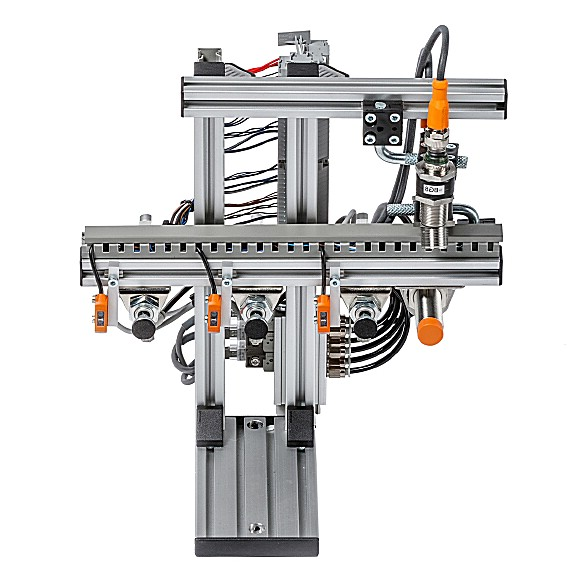
\includegraphics[trim={0 0 0 0},clip,width=8cm]{maquete/sensores/69511_3.jpg}
    % };
    % \draw[red,ultra thick,rounded corners] (0,0) rectangle (9.4,6.2);
    % \begin{scope}[x={(image.south east)},y={(image.north west)}]
        \draw[ultra thick,rounded corners] (3.5,4) rectangle (6.5,6);
        \draw (5,5) node {\textbf{Process}};
        \draw (0,5) node {\textbf{Inputs}};
        \draw[->,>=stealth, very thick] (1,4.5) -- ++ (2.5,0);
        \draw[->,>=stealth, very thick] (1,5)   -- ++ (2.5,0);
        \draw[->,>=stealth, very thick] (1,5.5) -- ++ (2.5,0);
        \draw (10,5) node {\textbf{Outputs}};
        \draw[->,>=stealth, very thick] (6.5,4.5) -- ++ (2.5,0);
        \draw[->,>=stealth, very thick] (6.5,5)   -- ++ (2.5,0);
        \draw[->,>=stealth, very thick] (6.5,5.5) -- ++ (2.5,0);
      % \end{scope}
    \end{tikzpicture}
  \caption{Input\slash Output Process model}
    \label{fig:ioProcModel}
\end{figure}


In some systems, its inputs and outputs can't represent it's behaviour, so the
concept of state is created, and it represents the behaviour of the system in a
given instant $t$.

The states can be continuous or discrete, and the systems which these states
represent can be considered as Continuous Systems, Discrete Systems or even
Hybrid Systems, which combine both kind of states.

The systems modelled in this work are Discrete Systems, more details about other
kinds of systems as well as examples and their analysis can be found on
\cite{oppenheim1996signals} and \cite{kalouptsidis1997signal}.
\section{Discrete Event Systems}
\label{sec:discreteEventSystems}
Discrete Systems can be driven by time and by events. It means, the states can
be changed continuously by the time or instantaneously by some ensemble of events.

In this thesis we are interested in the event-driven type. Some basic mathematical
formalisms, nomenclature and representations can be developed to facilitate the
understanding. Some of those will be presented in the following sections based
on \cite{cassandras2009introduction, david2005discrete,david1989grafcet}.
\section{Languages} \label{sec:automata} A language can be defined by the Merriam-Webster's dictionary as ``a systematic
means of communicating ideas or feelings by the use of conventionalized signs,
sounds, gestures, or marks having understood meanings'' And as it is defined by
this dictionary entry we pursue to communicate the complete behaviour of the
\DES. Firstly we need to define a group, or set of marks to characterise the
singular behaviour of the system. So, we define a set $\Sigma$. This set contains
all elements which combined can create a language. Again in analogy with
linguistics, each one of these marks, the events can be compared to letters ,
provided that $\Sigma$ can be called an ``alphabet'', and the combination of its
events ``words''. Words are also called ``strings '' or even ``traces''.
Considering the use of the word ``string'' as the variable type used on several
programming languages used in this work, we prefer the use of the vocables
``word'' and ``trace''. We can also define a mark to represent an empty word,
$\epsilon$, that is, a word that is not formed by any event.

The combination process to form words is called concatenation. For instance,
given two events $a$ and $b$, the words $ab$ and $ba$ can be created concatenating these two events and there is no particular reason to suppose that $ab$ is equal to $ba$, the same way the words ``ten'' and ``net'' have different meanings in English.

We can also concatenate two words, to create a different one, we can take the
words $ab$ and $ba$ and create words like $abba$ and $baab$.

As we extended the definition of concatenation to words, we define $\epsilon$,
the empty word, as the identity element of concatenation: $w\epsilon = \epsilon
w = w$ for any word $w$.

Likewise, we can define the length of a word as the number of events contained
by this word, we denote the length with two vertical bars, given a word $w$ its
length is equal to $|w|$ and by definition $|\epsilon| = 0 $.

As we know, there is a great number of human western languages, as portuguese,
english, french, spanish etc, that roughly are formed by the same alphabet, but
overall they are formed by different combination of words. Similar things can
happen with languages that define the \DESs, so we can define as in
\cite{cassandras2009introduction}.
% \pagebreak
\begin{definition}[Language]
  \label{def:language}~\\
  A Language defined over an alphabet $\Sigma$ is formed from finite-length
  words generated from the concatenation of the events in $\Sigma$ and
  $\epsilon$.
\end{definition}

Take for example an alphabet $\Sigma = \{a,b,g\}$, we can define different
languages
\begin{subequations}
  \begin{equation*}
  L_1=\{\epsilon, a, abb\}
  \end{equation*}
  \begin{equation*}
  L_2=\{\text{all possible words of length 3 starting with g}\}
  \end{equation*}
  \begin{equation*}
  L_3=\{\text{all possible words starting with g}\}
  \end{equation*}
\end{subequations}

The cardinality of this sets are $|L_1|=3$, $|L_2|=9$, $|L_3|=\infty$
As we can see from the same alphabet very different languages can be created, thus we can define a way to encapsulate all possible languages generated from
the same alphabet $\Sigma$. Let us denote by $\Sigma^*$ the set containing all
finite words composed with the elements of $\Sigma$ and $\epsilon$. The *
operation is called the \textit{Kleene-closure}. Similarly to $L_3$ it is
countably infinite since it contains arbitrarily long words. For instance the
\textit{Kleene-closure} of the alphabet $\Sigma = \{a, b, c\}$ is:
\begin{equation*}
  \label{eq:kleeneExample}
  \Sigma^* = \{\epsilon,a,b,c,aa,ab,ac,ba,bb,bc,ca,cb,cc,aaa,\dots\} 
\end{equation*}
There are a few operations with languages and alphabets that can be defined, but they are outside the scope of this work, they can be found on \cite{cassandras2009introduction}.
\section{Representation of Languages}
\label{sec:representationLanguages}

Although languages can describe the behaviour of \DESs, there are cases, as the
one shown
by the language $L_3$ in the last section, in which the language is enormous, in
that case countably infinite, what makes them not so simple to communicate the
behaviour of the system. For this purpose, there are some other formalisms that
aid the comprehension, since they can be a more compact way of expressing the
system's behaviour or accompanied by diagrams.

In the following subsections two of the most known representations will be
presented: Automata and Petri Nets.

% \pagebreak
\subsection{Automata}
\label{sec:automata}
One of the most known representation of languages are automata. The notion of
automaton is basically the definition of \DESs, as we saw in the
\autoref{sec:discreteEventSystems}: a set of events can change the state of the
system. If we know all the events composing the language of the
system and its states, we can have its alphabet $\Sigma$ and we can create a set $X$ composed
by all states.
From $\Sigma$ and $X$ we can derive a function that represents the transition
from a state to other, this function is called \emph{transition function} of the automaton
denoted as $f : X \times \Sigma \rightarrow X$. For example if a system have an
alphabet $\Sigma = \{a,b\}$ and 2 states, we can name the states $x$ and
$y$, and then create the set $X = \{x,y\}$. Knowing that the system begins at state $x$
and that when event $a$ happens it changes to state $z$ we can create a function
$f(x,a)$ and define it as $y$. Likewise if we know that when the system is at
state $y$ and event $b$ happens, a function $f(y,b)$ can be defined as $a$.

As a
visual aid, a representation of these functions can be made through a diagram, called \emph{state transition diagram}. In this kind of diagram the states are
represented by circles labeled with their names, and the functions as arcs
labeled with the corresponding event,connecting two states, with arrows in one of their
extremities indicating the transition from a state to other. The initial state
of the automaton has an arc pointing towards it coming from no other state.
\autoref{fig:functionDiagram} can represent the functions $f(x,a)$ and $f(y,b)$
described in the last paragraph.
\begin{figure}[H]
  \centering
  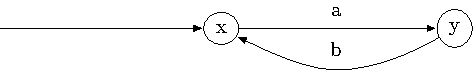
\includegraphics[width=0.3\textwidth]{automata/function/function.tikz}
  \caption{State Transition Diagram}
  \label{fig:functionDiagram}
\end{figure}
Now, for a more complex example, from \cite{cassandras2009introduction}:

\begin{example}[Simple Automaton] ~\\
  \label{ex:simpleAutomaton}
  Given $\Sigma = \{a,b,g\}$, $X = \{x,y,z\}$ and the following transition functions:
  \begin{align*}
   f(x,a)&=x&f(x,g)&=z\\
   f(y,a)&=x&f(y,b)&=y\\
   f(z,b)&=z&f(z,a)&=f(z,g)=y\\
 \end{align*}
\end{example}
We can represent this automaton with the diagram on \autoref{fig:diagramExapleAutomata}
\begin{figure}[H]
  \centering
  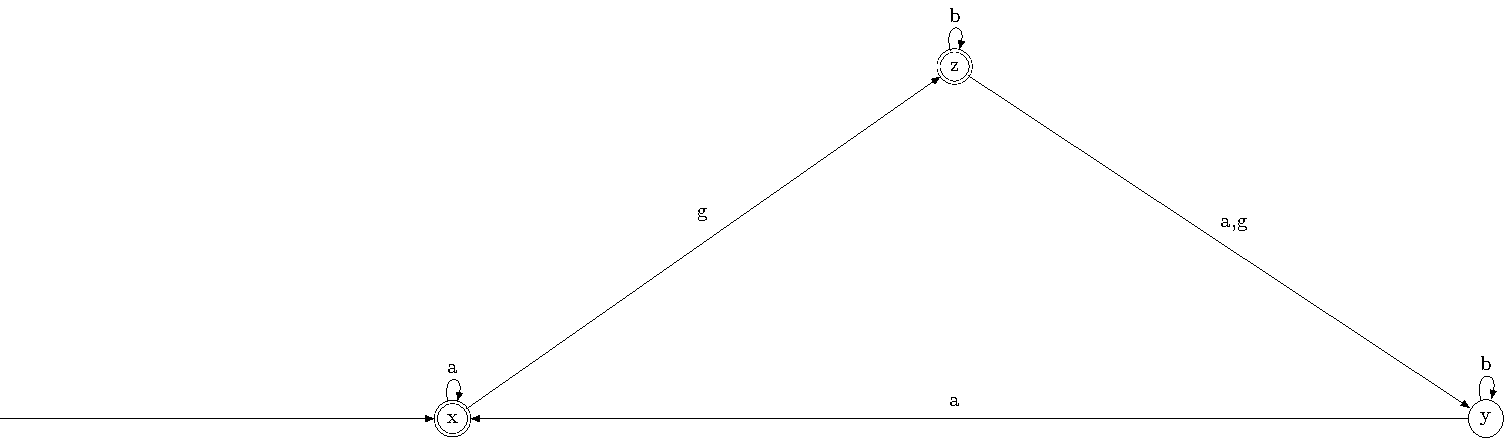
\includegraphics[width=0.5\textwidth]{automata/example/example.tikz}
  % \includetikzfigure[width=0.5\textwidth]{automata/example/example}
  \caption{Diagram representing the automaton from example \ref{ex:simpleAutomaton}}
  \label{fig:diagramExapleAutomata}
\end{figure}
We can also mark states that have some special meaning, a final state for instance. In this work, as in \cite{cassandras2009introduction} they are
  going to be identified by double circles.

  
  Now a deterministic Automaton can be defined:
\begin{definition}[Deterministic Automaton]
  \label{def:DeterministicAutomaton}~\\
  A Deterministic Automaton, denoted by G, is a five-tuple
  \[ G = (X,\Sigma,f, x_0,X_m)\] where:

  \indent X is the set of \textbf{states} \\
  \indent $\Sigma$ is the finite set of \textbf{events} associated with G\\
  \indent $f: X \times \Sigma \rightarrow X$ is the \textbf{transition function}  \\
  \indent $x_0$ is the \textbf{initial state} \\
  \indent $X_m \subseteq X $ is the set of \textbf{marked states}

\end{definition}


Other kinds of automata and operations between automata exist but are not going
to be used in this work, again \cite{cassandras2009introduction} present them.

\subsection{Petri Nets}
\label{sec:petriNets}
Another kind of representation of languages are Petri Nets, whose concept was created by C.A.Petri
in the early 1960's. Differently from the automata representation that are
basically formed from states, Petri nets are bipartite graphs, formed by nodes
called \emph{places} and \emph{transitions}.
Transitions represent the events that drive the system, and places represent the
conditions for these events to happen. The mechanism to represent the fulfilment
of the conditions
is named marking. A petri net is built over three basic concepts, the petri net
graph\slash structure, its marking and firing transitions.
The next subsections will be based on \cite{david2005discrete} and \cite{cassandras2009introduction}.

\subsubsection{Petri Net Graph}
\label{sec:petrinetGraph}
Similarly, arcs are used to connect
the nodes and have arrowheads to identify the direction,
but differently, all arcs must have exclusively one node at each end, that means
no arc is used to identify the initial state of a petri net. As said, a petri net is
bipartite graph, that means places can only connect to transitions and vice
versa. In this work as in \cite{david2005discrete} places will be represented by
circles and transitions by bars. 
\begin{figure}[H]
  \centering
  \begin{subfigure}[t]{0.45\textwidth}
  \centering
  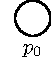
\includegraphics{petriNet/net/place.tikz}
  % \includetikzfigure[width=0.5\textwidth]{automata/example/example}
  \caption{A place.}
\end{subfigure}
~
\begin{subfigure}[t]{0.5\textwidth}
  \centering
  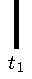
\includegraphics{petriNet/net/transition.tikz}
  % \includetikzfigure[width=0.5\textwidth]{automata/example/example}
  \caption{A transition}
\end{subfigure}
  \caption{Component nodes of a petri net.}  
\end{figure}

The same way a function was created to define the transitions of states in an
automaton, two functions will be created to define the connections between places
and transitions. First we need to define the sets of places and transitions. $P$
is the set of places and $T$ the set of transitions. With this two sets we can
then define those functions. The first one represents the arcs
from places to transitions, and is denoted as $Pre: P \times T \rightarrow
\{0, 1\}$, the second one the arcs that connects transitions to places, denoted
as $Post: P \times T \rightarrow \{0,1\}$. The value $1$ is attributed to arcs
that exist and $0$ to the nonexistent ones.


\begin{example}[Simple Petri Net structure] ~\\
  \label{ex:simplePetriNetStructure}
  Given $P = \{p_0,p_1\}$, $T = \{t_0,t_1,t_2\}$ and the following transition
  functions:
  \begin{align*}
   Pre(p_0,t_0)& = 0  &  Post(p_0,t_1) &= 0 & Pre(p_1,t_0) &= 0 &  Post(p_1,t_1) &= 1 \\
   Post(p_0,t_0) &= 0  &    Pre(p_0,t_2) &= 0   & Post(p_1,t_0) &= 0   & Pre(p_1,t_2) &= 0\\
   Pre(p_0,t_1) &= 0    &  Post(p_0,t_2) &= 0  &  Pre(p_1,t_1) &= 0     &Post(p_1,t_2) &= 0\\
  \end{align*}
  We can represent this petri net structure with the diagram on \autoref{fig:simplePetriNetStructure}
\end{example}
\begin{figure}[H]
  \centering
  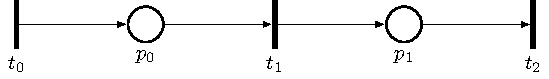
\includegraphics[width=0.5\textwidth]{petriNet/prepost/prepost.tikz}
  % \includetikzfigure[width=0.5\textwidth]{automata/example/example}
  \caption{Diagram representing the petri net structure from example \ref{ex:simplePetriNetStructure}}
\label{fig:simplePetriNetStructure}
\end{figure}
A drawback from the definition of this functions, is that is not possible to
have more than an arc linking two nodes, so we can generalize them to any natural number:
\begin{align*}
  Pre:  P \times T \rightarrow \mathbb{N}_0\\
  Post: P \times T \rightarrow \mathbb{N}_0
\end{align*}
with this new definition we can change the definition of $Post(p_1,t_1)$ from
$0$ to $2$ resulting on the following petri net structure.
\begin{figure}[H]
  \centering
  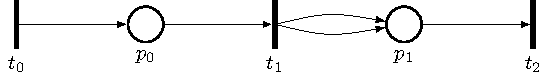
\includegraphics[width=0.5\textwidth]{petriNet/prepost/prepost2.tikz}
  % \includetikzfigure[width=0.5\textwidth]{automata/example/example}
  \caption{Diagram representing the petri net structure from example
    \ref{ex:simplePetriNetStructure}, but with $Post(p_1,t_1)=2$}
\label{fig:simplePetriNetStructureNatural}
\end{figure}
In order to reduce the number of arcs in a diagram, usually only one arc is
drawn and a label is added with the value of its respective function, if it is
greater than $1$, \autoref{fig:simplePetriNetStructureGeneralized} illustrates it:
\begin{figure}[H]
  \centering
  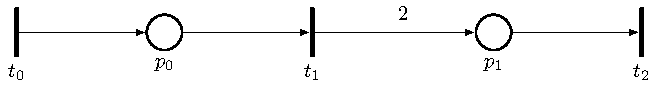
\includegraphics[width=0.5\textwidth]{petriNet/prepost/prepost3.tikz}
  % \includetikzfigure[width=0.5\textwidth]{automata/example/example}
  \caption{Same diagram as \autoref{fig:simplePetriNetStructureNatural} but with
    labeled arcs.}
\label{fig:simplePetriNetStructureGeneralized}
\end{figure}

\subsubsection{Marking}
\label{sec:marking}

As said in the beginning of this subsection marking is used as the mechanism to
represent if the condition of occurrence of a determined event is met or not.
But also it can be used to represent the state of the system. The mechanism
works as follows. Tokens can be designated to places and the way the tokens are
distributed among places is called the marking of a petri net graph. We can define a marking function $x :
P \rightarrow \mathbb{N}$ that denotes the number of tokens in a determined place.
In this
work, as in the majority of articles and books, the tokens will be
represented as black dots inside the places. 

The
\Autoref{fig:unmarked,fig:marked} show an unmarked and a marked petri net graph.
\begin{figure}[H]
\begin{subfigure}[t]{0.45\textwidth}
  \centering
  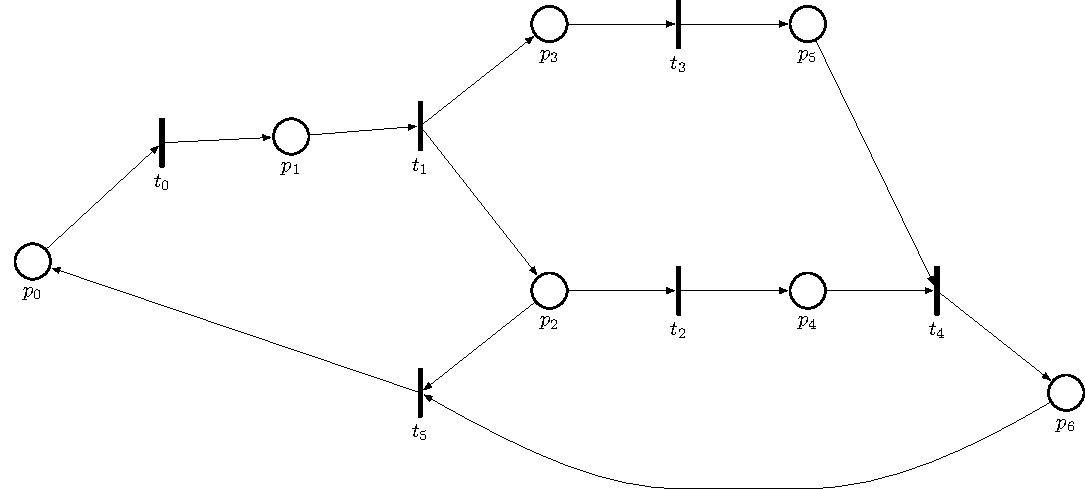
\includegraphics[width=\textwidth]{petriNet/net/unmarked.tikz}
  % \includetikzfigure[width=0.5\textwidth]{automata/example/example}
  \caption{Unmarked}
  \label{fig:unmarked}
\end{subfigure}
~
\begin{subfigure}[t]{0.45\textwidth}
  \centering
  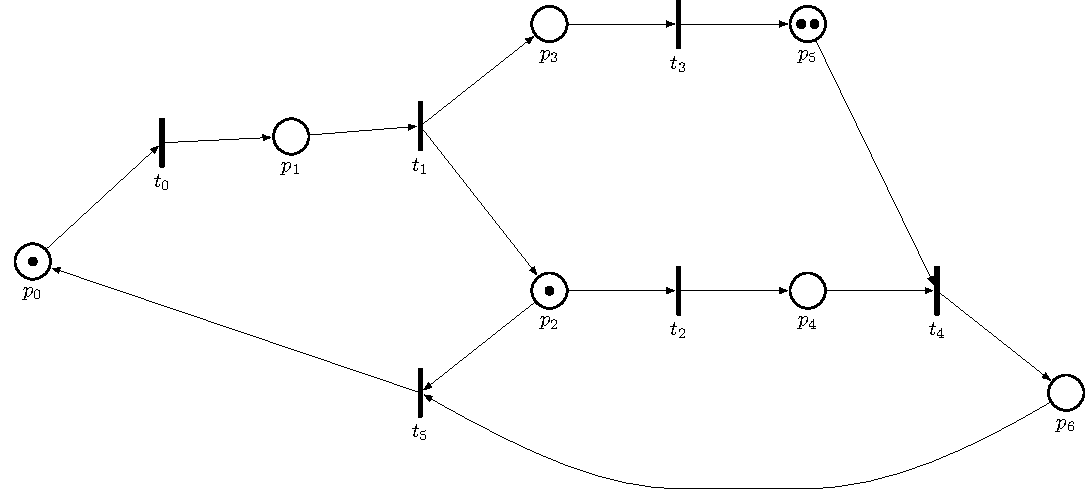
\includegraphics[width=\textwidth]{petriNet/net/marked.tikz}
  % \includetikzfigure[width=0.5\textwidth]{automata/example/example}
  \caption{Marked}
  \label{fig:marked}
\end{subfigure}
\caption{Example of unmarked and marked petri net graphs.}
\end{figure}

The marking of a petri net, can be represented as a
vector of the function $x$ applied on all places, for example the marking of the
\autoref{fig:marked} is the following vector $\mathbf{x}$

\begin{equation*}
\mathbf{x}=\begin{bmatrix}
  x(p_0)\\
  x(p_1)\\
  x(p_2)\\
  x(p_3)\\
  x(p_4)\\
  x(p_5)\\
  x(p_6)
\end{bmatrix} =
\begin{bmatrix}
  1\\
  0\\
  1\\
  0\\
  0\\
  2\\
  0
\end{bmatrix}
\end{equation*}

This vector $\mathbf{x}$, the marking of the petri net, can be identified as the
state of the petri net. So, different configurations of tokens mean different
states of the system, now we only need a way to change from a state to other, in
other words, move the tokens.

\subsubsection{Firing Transitions}
\label{sec:firingTransitions}
The mean of move the tokens is firing transitions. When an event  happens and
the corresponding transition is enabled, this transition is fired and tokens
are moved between places.
We can define the functions $I : T \rightarrow 2^P$ and $O : T \rightarrow 2^P$ that
describe the set of places considered as inputs and outputs of a transition: 
\begin{align*}
  I(t_j)= \{p \in P : Pre(p,t)> 0\}\\
  O(t_j)= \{p \in P : Post(p,t)> 0\}\\
\end{align*}
\begin{definition}[Enabled transition]
  \label{def:enabledTransition}~\\
  A transition is enabled if
  \[ x(p_i)\geq Pre(p_i,t_j) \text{ for all }{p_i \in I(t_j)}\]
  if $I(t_j)=\emptyset$, $t_j$ is always enabled. 
\end{definition}

And we can define the dynamic of the petri net, how the tokens move: 

\begin{definition}[Petri net dynamics]
  \label{def:petriNetDynamics}~\\
   It is possible to define a \emph{state transition}
  function, $f : \mathbb{N}^n \times T \rightarrow \mathbb{N}^n$  , where $n$ is
  the length of the state vector $\mathbf{x}$. This function $f$ is defined for
  a transition $t_j \in T$ if and only if this transition is enabled. If
  $f(\mathbf{x},t_j)$ is defined, then we create a new state vector
  $\mathbf{x}^\prime$:

  \[ x^\prime(p_i) = x(p_i) - Pre(p_i,t_j) + Post(p_i,t_j), i=1,\dots n \]
\end{definition}
  
As an example we can take \Autoref{fig:petriNetDynamics}:
\begin{figure}[H]
  \centering
 \begin{subfigure}[t]{0.45\textwidth}
  \centering
  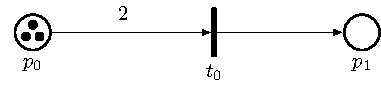
\includegraphics{petriNet/net/beforeFiring.tikz}
  % \includetikzfigure[width=0.5\textwidth]{automata/example/example}
  \caption{Before firing.}
  \label{fig:beforeFiring}
\end{subfigure}
~
\begin{subfigure}[t]{0.45\textwidth}
  \centering
  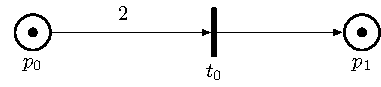
\includegraphics{petriNet/net/afterFiring.tikz}
  % \includetikzfigure[width=0.5\textwidth]{automata/example/example}
  \caption{After firing.}
  \label{fig:afterFiring}
\end{subfigure}
  \caption{Example of petri net Dynamic.}
  \label{fig:petriNetDynamics}
\end{figure}
The state before firing transition $t_0$ is $\mathbf{x}=\begin{bmatrix}3&
  0\end{bmatrix}^T$ and as we see $Pre(p_0,t_0)=2$ and $Post(p_1,t_0)=1$ so
applying the petri net dynamic we can find the next state $\mathbf{x}^\prime=\begin{bmatrix}1&
  1\end{bmatrix}^T$

Once all these fundamentals are presented we can finally define a Petri Net

\begin{definition}[Petri net]
  \label{def:petriNet}~\\
  A Petri net is defined as a five-tuple
  \[PN = (P,T,Pre,Post,\mathbf{x}_0)\]
  where: \\
  \indent $P$ is the set of \textbf{places} \\
  \indent $T$ is the set of \textbf{transitions} \\
  \indent $Pre$ is the \textbf{input incidence} function  \\
  \indent $Post$ is the \textbf{output incidence} function\\
\indent $\mathbf{x}_0$ is the initial marking of the net \\
And its dynamic is ruled by the \emph{state transition} function $f$ defined at \ref{fig:petriNetDynamics}.

\end{definition}

To make the connection between the Petri net and the events of the system, called $\Sigma$, the alphabet, we can
define a labeling function, $l : T^* \rightarrow \Sigma^*$ that makes the link between a
sequence of firing transitions and a sequence of events. But each transition
can only have one respective event. 

\begin{definition}[Labeled Petri net]
  \label{def:petriNet}~\\
  A Labeled Petri net is defined as a seven-tuple
  \[PN = (P,T,Pre,Post,\mathbf{x}_0,\Sigma,l)\]
  where: \\
  \indent $(P,T,Pre,Post,\mathbf{x}_0)$ is a Petri Net\\
  \indent $\Sigma$ is the set of \textbf{events} \\
  \indent $l$ is the \textbf{labeling} function  \\
\end{definition}

Usually the events are represented in the petri net graph over its respective
transition as shown in the \autoref{fig:labeledPetriNet}. This system has an alphabet
$\Sigma=\{a,b\}$ and labeling functions $l(t_0)=a$ and $l(t_1)=b$.

\begin{figure}[H]
  \centering
  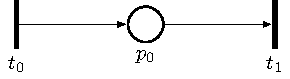
\includegraphics{petriNet/labeled/labeled.tikz}
  % \includetikzfigure[width=0.5\textwidth]{automata/example/example}
  \caption{Labeled Petri net.}
  \label{fig:labeledPetriNet}
\end{figure}

\section{Control Interpreted Petri Nets}
\label{sec:cipn}
One of the greatest uses of Petri Nets, besides modeling a system, is its
ability to model the control of a system. For this intent we use Control Interpreted Petri nets. It is an
extension from the labeled Petri net, we add actions for places, so it is
possible to change the outputs of the system, conditions to the transitions, so it
is possible to change the state of the control based on the inputs of the
system, and even the ability to delay the firing transitions based on time.
Another artifice used is an inhibitor arc, that prevents the firing of a
transition based on the marking of the corresponding place.

\begin{definition}[Control Interpreted Petri net]
  \label{def:cipn}~\\
  A Labeled Petri net is defined as a seven-tuple
  \[PN = (P,T,Pre,Post,\mathbf{x}_0,In,\Sigma,C,l_C,D,L_D,A,I_A)\]
  where: \\
  \indent $(P,T,Pre,Post,\mathbf{x}_0)$ is a Petri Net\\
  \indent $In$ is the \textbf{inhibitor arc} function that prevents the
  enablement of transitions \\
  \indent $\Sigma$ is the set of \textbf{events} associated to transitions \\
  \indent $C$ is the set of \textbf{conditions} associated to transitions \\
  \indent $l_C$ is the \textbf{labeling} function that associates a transition
  with events and conditions from $\Sigma$ and $C$\\
  \indent $D$ is the set of \textbf{delays} associated to transitions \\
  \indent $l_D$ is the \textbf{labeling} function that associates a transition with a delay from $D$ \\
  \indent $A$ is the set of \textbf{actions} associated to places \\
  \indent $l_A$ is the \textbf{labeling} function that assigns actions from $A$ to a place \\
\end{definition}
The definition of $In : (P \times T )\rightarrow\mathbb{N}$ is that a transition
$t_j$ is inhibited if $x(p_i)\geq In(p_i,t_j)$. Inhibitor arcs are not used in
this work but usually they are represented with an arc with a circle in one of
its ends, as shown in \autoref{fig:inhibitor}.

\begin{figure}[H]
  \centering
  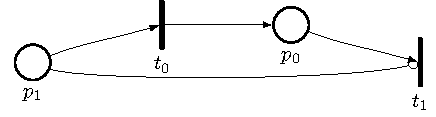
\includegraphics{petriNet/inhibitor/inhibitor.tikz}
  % \includetikzfigure[width=0.5\textwidth]{automata/example/example}
  \caption{Example of Petri net with inhibitor arc.}
  \label{fig:inhibitor}
\end{figure}
As we can see from the definition there are two labeling functions to connect 
transitions, $l_C$ and $l_D$. The $l_c$ is defined for transitions with no
firing delay and $l_D$ for transitions with firing delay.

The labeling function $l_C : T^0\rightarrow(\Sigma \times C)$ defines a pair of
event and boolean condition from $\Sigma$ and $C$ respectively. A transition
$t_i$ belonging to $T^0$ (a subset of $T$ that represents the transitions with
no time delay) has a corresponding event, condition tuple $(\sigma_i,c_i)$
For example, take a transition $t_0$, $\Sigma =\{\sigma_0\}$ and $C=\{c_0\}$. If
a function $l_c(t_0)=(\sigma_0,c_0)$ is defined, this transition will be fired
when the condition $c_0$ is true and the event $\sigma_0$
happens, but obviously, if and only if this transitions is enabled and not
inhibited. The transition $t_0$ is represented graphically as shown in \autoref{fig:condition}

\begin{figure}[H]
  \centering 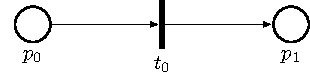
\includegraphics[width=0.3\textwidth]{petriNet/cipn/condition.tikz}
  \caption{Representation of new labeling function}
  \label{fig:condition}
\end{figure}

If the event is missing from the representation of the transition, it is equal
to the $\lambda$
, the always occurring event. And if the condition is missing, that means it is
equal to $1$, it is always $true$. If both are missing, that means the
transition will be automatically executed if it is enabled. 

By the other hand, the labeling function $l_D : T^D \rightarrow D$, defines a delay for the
transition to be fired. A timed transition $t_i$, a transition in $T^D$ (a subset of T
that represents the transitions with a time delay), has a corresponding delay
$d_i$. As an example, take a timed transition $t_1$ and $D=\{d_1\}$, after the
enablement of the transition, it takes $d_1$ time units in order to be fired. In
this work timed transitions are represented as bars slightly larger than normal
conditions. An example of this representation we can see \autoref{fig:timedtransition}

\begin{figure}[H]
  \centering 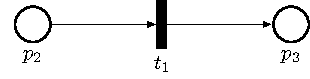
\includegraphics[width=0.3\textwidth]{petriNet/cipn/timedtransition.tikz}
  \caption{Representation of a timed transition.}
  \label{fig:timedtransition}
\end{figure}
Another labeling function that was created is $l_A : P\rightarrow 2^A$,
assigning a set of actions belonging to $A$ to a place. Actions can be impulse actions or continuous. A
continuous action happens always that the marking of a place is greater than 0,
$x(p_i)>0$, an impulse action, on the other hand, happens only when the marking of
the place changes from 0 to a value greater than 0. 
Actions are represented graphically as labels in places. Impulse actions are differed by a star (*) at its end. So an action $F$ is
continuous and $B^*$ is an impulse action. 
\autoref{fig:actions} show a representation of a Place with both kinds of actions.
\begin{figure}[H]
  \centering 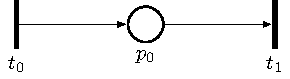
\includegraphics[width=0.3\textwidth]{petriNet/cipn/actions.tikz}
  \caption{Representation of labeling of Actions.}
  \label{fig:actions}
\end{figure}

Although these representations exist, in this work events, conditions and
actions labels are suppressed from the diagrams and tables accompany the drawings
showing the meaning of the transitions (firing events and conditions) and places
(Actions). This choice was made because when the controlled interpreted Petri nets
are very
large as the ones shown in the next chapters, if the events, conditions and
actions labels are long they can increase the size of the
diagram.

To illustrate this better we give an example based on one example from \cite{david1989grafcet}.
\begin{example}[Loading of a wagon] ~\\
  \label{ex:loadingOfAWagon}
We consider the system represented by the scheme in
\autoref{fig:cipnexamplescheme}. A wagon can be moved between the points $a$ and
$b$, using the inputs $L$ and $R$ (moving it to the left or right,
respectively). At point $a$ there is a button $m$ that can be pressed by an
operator and a limit switch called $a$ that is activated when the wagon is on
the left. At point $b$, an homonym limit switch is placed and activated when the
wagon is on the right. There is a hopper that can
be opened when the input $Open$ is turned on and closed when not.If it is opened
its content is poured. There is also a
button $p$ that is activated when the weight applied over the plate is equal or
greater to the weight of a full wagon. 

The objective of the control is, when the wagon is in its leftmost position and
the button $m$ is pressed, it moves to the right, stops at $b$, the hopper is
opened and the wagon is loaded, when it is completely full it moves to the left
and it stops at $a$ waiting to be unloaded and for a next press of $m$ to recommence
the loop. 
\end{example}


\begin{figure}[H]
  \centering \includegraphics[width=0.8\textwidth]{cipnExample/scheme.tikz}
  \caption[cipnexample]{Example of System to be controlled by the Petri Net}
  \label{fig:cipnexamplescheme}
\end{figure}
From the description of the control it is possible to create a Control Interpret
Petri Net to describe it, as the one in \autoref{fig:cipnexample}


\begin{figure}[H]
  \centering 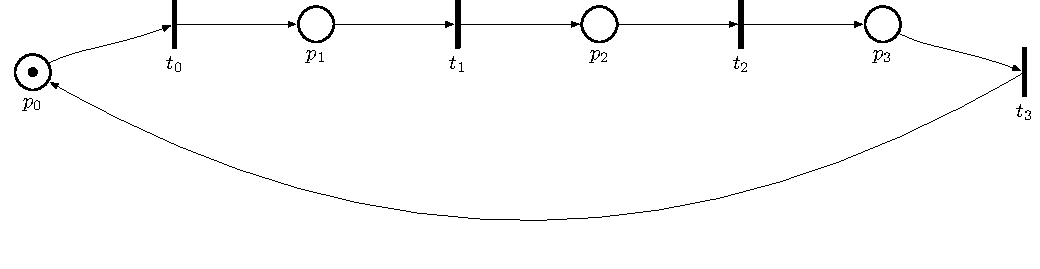
\includegraphics[width=0.8\textwidth]{cipnExample/cipn.tikz}
  \caption[cipnexample]{Example of Control Interpreted Petri Net to control
    system in \autoref{fig:cipnexamplescheme}}
  \label{fig:cipnexample}
\end{figure}

The meaning\slash description of each place and transition is given by the
following tables:

\begin{table}[htbp]
\caption{Control Interpreted Petri Net Example Places.}
\centering
\begin{tabular}{M{5cm}M{10cm}}
Places & Meaning\\
\hline
\hyperlink{cipnExampleNet:p0m1}{\hypertarget{cipnExampleTable:p0m1}{$p_{0}$}} & System Stopped\\
\hyperlink{cipnExampleNet:p1}{\hypertarget{cipnExampleTable:p1}{$p_{1}$}} & R (Car Moving to the Right)\\
\hyperlink{cipnExampleNet:p2}{\hypertarget{cipnExampleTable:p2}{$p_{2}$}} & Open (Container Opened)\\
\hyperlink{cipnExampleNet:p3}{\hypertarget{cipnExampleTable:p3}{$p_{3}$}} & L (Car Moving to the Left)\\
\end{tabular}
\end{table}

\begin{table}[H]
\caption{Control Interpreted Petri Net Example Transitions.}
\centering
\begin{tabular}{M{5cm}M{10cm}}
Transitions & Meaning\\
\hline
\hyperlink{cipnExampleNet:t0}{\hypertarget{cipnExampleTable:t0}{$t_{0}$}} & m (filling request)\\
\hyperlink{cipnExampleNet:t1}{\hypertarget{cipnExampleTable:t1}{$t_{1}$}} & b (Right Limit Switch)\\
\hyperlink{cipnExampleNet:t2}{\hypertarget{cipnExampleTable:t2}{$t_{2}$}} & p (Car is Full)\\
\hyperlink{cipnExampleNet:t3}{\hypertarget{cipnExampleTable:t3}{$t_{3}$}} & a (Left Limit Switch)\\
\end{tabular}
\end{table}


In this work as in the usual boolean notation, when just the name of a variable is given in a table it means the
variable is equal to true, and when there is a bar in its top it is equal to
false, so they determine conditions. E.g.: $b$ and $\overline{b}$.
And when a variable is preceded by $\uparrow$ and $\downarrow$, they  determine
events corresponding to its raising and falling edge.

\usetikzlibrary{arrows,shapes,circuits.plc.ladder,external}

\section{Implementation of Control Interpreted Petri Nets}
\label{sec:implementPetriNets}
Once the control of a system is modeled by a \CIPN, it
is needed to implement the control in a real controller. The most used
controllers in the industry are \PLCs. The international standard IEC 61131,
defines all the standards for \PLCs, and its third part (IEC 61131-3) defines
five languages to program \PLCs: \LD, Function Block Diagram
(FBD),  Structured Text (ST), Instruction List (IL) and Sequential Function
Chart (SFC). One of the most used in the industry is \LD, because of its
resemblance with electric connections. So we are going to use \LD{} to implement the
control designed with the \CIPN.

\subsection{Ladder Logic}
\label{sec:ladder}

The ladder logic is based on two components, contacts and coils. Their terminals are
interconnected to transmit boolean signals. This connection is similar to the
ladder physical implementation, from where came its inspiration, the components
were connect to boards and they formed electric circuits, turning on and off
motors and other actuators, based on the combination of its inputs. The name
Ladder comes from the resemblance between its structure (circuits formed in
parallel one above the other) and a ladder, so each circuit is called a Rung by analogy. The logic
values in a \LD{} rung
are transmitted from the left to the right of the diagram. The components let
the logic ``current'' flow from its left terminal to the right terminal
depending on some conditions, and these conditions vary from component to
component.
The rungs are executed one by one and once the very last rung is executed,
the first rung is re-executed, thus creating an infinite loop. 
 The graphical representation of the most used types of contacts and coils
can be seen in \Autoref{fig:contacts,fig:coils}

\newlength{\ladderskip}
\newlength{\ladderrungsep}

% Types of Contacts
\begin{figure}[H]
\begin{subfigure}[t]{0.45\textwidth}
  \centering \includegraphics{ladder/contactNO.tikz}
  \caption{Normally Opened Contact.}
  \label{fig:contactNO}
\end{subfigure}
~
\begin{subfigure}[t]{0.45\textwidth}
  \centering \includegraphics{ladder/contactNC.tikz}
  \caption{Normally Closed Contact.}
  \label{fig:contactNC}
\end{subfigure}
\vspace{1em}

\begin{subfigure}[t]{0.45\textwidth}
  \centering \includegraphics{ladder/contactP.tikz}
  \caption{Positive Edge Contact.}
  \label{fig:contactP}
\end{subfigure}
~
\begin{subfigure}[t]{0.45\textwidth}
  \centering \includegraphics{ladder/contactN.tikz}
  \caption{Negative Edge Contact.}
  \label{fig:contactN}
\end{subfigure}

  \caption{Types of Contacts.}
  \label{fig:contacts}
\end{figure}

% Types of Coils
\begin{figure}[H]
\begin{subfigure}[t]{0.45\textwidth}
  \centering \includegraphics{ladder/coilNO.tikz}
  \caption{Coil.}
  \label{fig:contactNO}
\end{subfigure}
~
\begin{subfigure}[t]{0.45\textwidth}
  \centering \includegraphics{ladder/coilNC.tikz}
  \caption{Negated Coil.}
  \label{fig:contactNC}
\end{subfigure}
\vspace{1em}

\begin{subfigure}[t]{0.45\textwidth}
  \centering \includegraphics{ladder/coilSet.tikz}
  \caption{Set (latch) Coil.}
  \label{fig:contactP}
\end{subfigure}
~
\begin{subfigure}[t]{0.45\textwidth}
  \centering \includegraphics{ladder/coilReset.tikz}
  \caption{Reset (unlatch) Coil.}
  \label{fig:contactN}
\end{subfigure}

  \caption{Types of Coils.}
  \label{fig:coils}
\end{figure}

\subsubsection{Contacts}
Contacts represent the conditions of the ladder logic depending on inputs. These inputs can be any variable in a
\PLC, an external input ( sensors of the system to be controlled), a variable stored in memory or the current
value sent to an output from the \PLC. A normally opened contact
activates its right terminal (set it to $true$) if the logic value in its left terminal
is $true$ and its corresponding input is equal to $true$ 
A normally closed contact activates its right terminal if the logic value in its
left terminal is $true$ and its corresponding input is equal to $false$.
The Positive Edge contact activates its right terminal only in the instant that
its input change from logic value $false$ to $true$, if the logic value in its
left terminal is $true$. And the Negative Edge contact activates its right
terminal only in the instant that its input change from logic value $true$ to
$false$.

As we can see, positive and negative contacts can be used to represent raising ($\uparrow$)
and falling edge  ($\downarrow$) events and normally opened and closed contacts
to represent conditions (and their negation).

\subsubsection{Coils}

Coils, by the other side represent the actuation in outputs. These
outputs can be a variable stored in memory or the outputs
of the controller (actuators of the system to be controlled, for instance). 
A coil sets its output variable to true if the logic value of its left terminal is $true$,
and sets the output to $false$ otherwise.
A negated coil does the exact opposite, sets the output value to true if the logic
value of its left terminal is $false$ and sets it to $true$ if the logic is
$true$.

A set coil (or latch) sets its output variable to $true$ if the logic value of its
terminal is $true$ and it remains $true$ until the variable is reset.
And a reset coil (or unlatch) sets its output variable to $false$ if the logic
value of its terminal is $true$ and it remains $false$ until the variable is
set.

\subsubsection{Combinational Logic}
In boolean logic, in order to show functional completeness, it is need to show a
complete set of connectives ( a set that can create all other logic connectives
as a combination of its elements ). A well-know complete set is $S=\{AND,NOT\}$,
binary conjunction and negation.
To show that the ladder logic is functional complete we need only to present how
to construct this two connectors in it.
The conjunction of two inputs, can be made using two contacts in series, as
shown in \autoref{fig:ladderSeries}
\begin{figure}[H]
  \centering \includegraphics{ladder/series.tikz}
  \caption{And logic in a Ladder rung.}
  \label{fig:ladderSeries}
\end{figure}
In this case C will only be activated if A and B are equal to $true$. ($C=AB$)

The negation of a variable can be achieved by the use of a normally closed
contact (\autoref{fig:ladderNot}).
\begin{figure}[H]
  \centering \includegraphics{ladder/not.tikz}
  \caption{Not logic in a Ladder rung.}
  \label{fig:ladderNot}
\end{figure}
C will only by activated if A is $false$. ($C=\overline{A}$)

Although all logic connectives can be constructed with this two connectors, the
OR connector can be achieved by the use contacts in parallel (\autoref{fig:ladderParallel}).
\begin{figure}[H]
  \centering \includegraphics{ladder/parallel.tikz}
  \caption{Or logic in a Ladder rung.}
  \label{fig:ladderParallel}
\end{figure}



\subsubsection{Function Blocks and extensions}
In order to increase functionality some function blocks and 
extensions to contacts were created. We can see examples of theses blocks and
contacts in the next figure:

\begin{figure}[H]
   \centering
\begin{subfigure}[t]{0.45\textwidth}
  \centering \includegraphics{ladder/ctu.tikz}
  \caption{Up counter.}
  \label{fig:ctu}
\end{subfigure}
~
\begin{subfigure}[t]{0.45\textwidth}
  \centering \includegraphics{ladder/ton.tikz}
  \caption{On-delay timer.}
  \label{fig:ton}
\end{subfigure}

\begin{subfigure}[t]{0.45\textwidth}
  \centering \includegraphics{ladder/comp.tikz}
  \caption{Less or equal comparator.}
  \label{fig:comp}
\end{subfigure}
  \caption{Examples of function blocks.}
  \label{fig:functionBlocks}
\end{figure}

Up counters (\autoref{fig:ctu}) save the value of a counter in a $CV$ variable. Every raising edge
on input $CU$ it increments $CV$ value. If $CV=PV$, the logic value of output $Q$ 
is set to $0$. When the input $R$ is true $CV$ value is set to $0$ and the
output $Q$ set to false.

On-delay timers (\autoref{fig:ctu}) set a timer when input $IN$ is $true$
and save it to $ET$. If $ET=PT$, the logic value of output $Q$ is set to $true$.
But if, meanwhile the counting, the value of $IN$ returns to $false$, $ET$ is reset to
$0$.

Comparator contacts as the less or equal comparator in \autoref{fig:comp}, work
similarly to contacts, but instead of an input as a condition, there are two
inputs ($value1$ and $value2$) and the condition is a comparison between both of
them. In this case, the contact is activated once its left terminals' logic
value is $true$ and $value1\leq value2$.

Other blocks and functions can be found in the IEC 61131-3, as adders,
subtractors, communication blocks etc.

\subsection{Conversion from \CIPN{} to \LD}
\label{sec:cipnToLD}

A simple method of conversion from \CIPN{} to \LD{} is presented in
\cite{moreira2013bridging}.

It consists in dividing the \CIPN{} in 4 modules:
\begin{enumerate}
\item A module of external events\\
  To create conditions to the firing of transitions based on external events
  (inputs)
\item A module of firing conditions\\
  To indicate what condition will be fired using the $Pre$, and $In$ functions, the conditions found on the
  last module and time delays (if it is a timed transition 
  )
\item A module of Petri Net dynamics\\
Uses the $Pre$ and $Post$ functions to determine the tokens ``motion''
\item A module of actions\\
  Determines the places where each action is performed.
\end{enumerate}
In this work, the external events and firing conditions was combined in order to
reduce the size of the program. But every module will be described as in
\cite{moreira2013bridging}.

\subsubsection{External events}
As external events are associated with positive and negative edge of the inputs
of the system, in this module, positive and negative edge contacts are used to
detect the rising and falling edge events, and they are stored in variables
using coils, a variable is created for every event.
For visibility's and organisation's sake a rung is used for each event,
resulting $|\Sigma|$ rungs. 
\subsubsection{Firing Conditions}
As said in \ref{sec:cipn}, for a transition $t_j$ to be fired, first it needs to be
enabled ($x(p_i)\geq Pre(p_i,t_j)$ for all $p_i\in I(t_j)$), not inhibited
($x(p_i)< In(p_i,t_j)$ for all $p_i\in I(t_j)$) and the conditions and events
$\sigma_jc_j$ are met or the delay $d_j$ is elapsed, depending on the kind of
transition.
As places can have multiple tokens, we can use $int$ variables to store the
number of tokens, and comparator contacts to determine if the transitions are
enabled and not inhibited.
When a place can only bear at most one single token for all markings of the
Petri net, a $bool$ variable can be used to store the number of tokens, in this
case a single normally open contact can be used to determine if there is a token
in that place.
The time delays are implemented using on-delay
timers. The state of fulfilment of the conditions is stored in variables, one
for each transition.
Similarly, for organisation's sake a rung is used for each transition, resulting
$|T|$ rungs.
\subsubsection{Petri Net Dynamics}
In this module the dynamic of the tokens is implemented. If the condition for
the firing of a transition is fulfilled (represented by normally open contacts), adders and subtractors
can be used to represent the movement of tokens, increasing and decreasing the
values from the $int$ variables that represent the marking
of each place, if their capacity is greater than one, if not they are
represented by boolean variables, and instead Set and Reset coils can be used to
represent a token entering a place and a token exiting another, respectively.
Again, for organisation's sake a rung is associated for each transition,
resulting $|T|$ rungs.

\subsubsection{Actions}
In the Action module, we use coils to act on the outputs. Depending on the type
of action and the logic of the control, set\slash reset coils or normal coils
can be used. The condition to activate\slash deactivate the output is the
presence of a token in the places where the action is performed, this can be
achieved by comparing the numbers of tokens in a place. If the tokens of a
place is represented by an $int$ variable, we use greater or equal comparators,
but if it is represented by a $bool$ variable, a normally opened contact is
enough. If the action is an impulse action we can put a positive edge in series
with the places contact or the comparator.

Differently from the original article, we will use one rung per
each action in A, resulting in $|A|$ rungs. This is made because in
\cite{renault2017regles} it is recommended to perform an action in only one
rung, and group the conditions using OR connectors.
In the industry this is important in order to reduce errors and to ease the
debugging process.

\subsubsection{Example}

An example of this conversion can be given using the same \CIPN{} from example 
\ref{ex:loadingOfAWagon}. As said, the external events and firing condition
modules are grouped in same module in this work. The converted Ladder Logic
can be seen in \autoref{fig:cipnexampleLadder}.
\begin{figure}[H]
  \centering \includegraphics{cipnExample/cipnLadder.tikz}
  \caption[cipnexample]{Example of Control Interpreted Petri Net converted to
    Ladder.}
  \label{fig:cipnexampleLadder}
\end{figure}

\subsection{Petri Net divided in multiple PLCs}
\label{sec:multiplePlcs}
A problem that can occur, is the case where a \CIPN{} must be divided in
multiple \PLCs, because of how the assembling of the plant was (some
inputs\slash outputs are only
connected to a single \PLC, and other inputs\slash outputs to another \PLC),
this division can be arbitrarily decided by the
person who will implement the control.

In \autoref{fig:communicationPlcPN}, it is shown an example of a \CIPN{} divided
between 2 \PLCs.
As we can see, in \Autoref{fig:communicationPlcPN1,fig:communicationPlcPN2}
there are dotted transitions and places. In this work, we will represent as
dotted, transitions and places that are part of another section of the Petri
Net. They are not represented in the same figure, 
but the arcs show the connection between the sections of the net, showing that
when connected they form a complete Petri net. In the digital form\footnote{Available at: \url{https://github.com/Accacio/docsTCC/raw/master/monografia.pdf}}  of this thesis it is possible to travel between
figures that are not in the same page just by clicking in the name of the
corresponding dotted place\slash transition.
\begin{figure}[H]
  \centering
  \begin{subfigure}[t]{0.5\textwidth}
    \center
    \includetikzfigure[width=\textwidth]{communicationPlcPN/communicationPlcPN}
    \caption{Petri Net on PLC 1.}
    \label{fig:communicationPlcPN1}
  \end{subfigure}%
  ~
  \begin{subfigure}[t]{0.5\textwidth}
    \centering
    \includetikzfigure[width=\textwidth]{communicationPlcPN/communicationPlcPN1}
    \caption{Petri Net on PLC 2.}
    \label{fig:communicationPlcPN2}
  \end{subfigure}
  \caption{Example of Petri Net divided between 2 PLCs.}
  \label{fig:communicationPlcPN}
\end{figure}

In order to solve the problem of communication caused by the division, there are
different ways, one of them is the method shown by \cite{antunesfloriano2019sincronizacao}, where
different sections are synchronised in a distributed manner using common places.
In this work, a master\slash slave approach was used. CLP1 was considered as the
master and CLP2 as a slave. For the master, it is created another module
called ``Data Sending\slash Receiving'', divided in 2 parts, the first that
happens before all other modules, with the objective of getting all needed
variables from other \PLCs, and another part, that happens after all other
modules, with the objective of sending variables to all other \PLCs.
By the other side, the slaves have 2 modules, one at the beginning, called
``Prepare Received Data'' and another at the very end called ``Prepare Data to
Send'', in which the data received from the master is prepared to be used and
the data is prepared to be sent to master.

The communication between \PLCs{} can be made using Profinet protocol, and if we
take for instance Siemens \PLCs, they have two function blocks called ``Get'' and
``Put'', that are used to establish data transfer between two \PLCs{} using the
Profinet protocol. Tutorials on how to configure this blocks can be found on \citep{antunesfloriano2019sincronizacao,oliveira2016protocolo,rochapereira2019automacao}.


The basic idea is to transfer the state of the variables that determine the
conditions of firing transitions between both \PLCs. The problem is that as the
two \PLCs are not in sync, the condition of a firing transition could change in
the middle of the logic. So, in order to circumvent it, we can duplicate those
variables in the slave PLC, and in the ``Prepare Received data'' module update
the values of these variables (using positive edges contacts), forcing them to
be updated only once in each loop and when their value are changed from $0$ to
$1$.

When a transition change the value of tokens in more than one \PLCs, as $t_1$,
an auxiliary variable is created in order to create a kind of
acknowledgement\slash permission 
from the master, as an ``ok, you can proceed'' to the slaves to perform the
dynamic of that transition.

The example of those three new modules are shown in \autoref{fig:communicationPlcPNLadder}

\begin{figure}[H]
  \centering
  \begin{subfigure}[t]{0.45\textwidth}
    \centering
    \includegraphics{communicationPlcPN/communicationPlcPNLadder.tikz}
    \caption{Ladder Logic on PLC 1.}
    \label{fig:communicationPlcPN1Ladder}
  \end{subfigure}%
  \hfill
  \begin{subfigure}[t]{0.45\textwidth}
    \centering
    \includegraphics{communicationPlcPN/communicationPlcPN1Ladder.tikz}
    \caption{Ladder Logic on PLC 2.}
    \label{fig:communicationPlcPN2Ladder}
  \end{subfigure}
  \caption{Example of Petri Net divided between 2 PLCs.}
  \label{fig:communicationPlcPNLadder}
\end{figure}
  
As we can expect, this kind of logic of master\slash slave works well when
there are 2 \PLCs, but when there are more \PLCs, this centralised approach
creates a single point of failure and as the master \PLC{} works as a hub, it
increases the communication delay. When there are more than two \PLCs{} it is
preferable to use a distributed approach as the one shown in
\cite{antunesfloriano2019sincronizacao}.

\section{Identification}
\label{sec:identification}

Once the control is implemented and the system is working as it should, we
arrive at the objective of this work, the identification of the system.
As said in the introduction, this work is based on \cite{moreira2018enhanced}.
In this article, a new model for \DES{} identification is proposed, called
\glsreset{DAOCT}\DAOCT. This model was created with aim of fault detection based
on the observation of the fault free behaviour of the system, as in the models
proposed by 
\cite{roth2009fdi} and \cite{klein2005fault}, but its use of paths increases the
efficiency for fault detection when compared with the latter articles.

This fault free observation is made by the acquisition of the observable signals
of the system (controller inputs and outputs) for a sufficiently long
period of time while the system works normally. These signals can be seen on \autoref{fig:obsSignals}.

\begin{figure}[H]
  \centering
  \begin{tikzpicture}
        % \draw[help lines,xstep=1,ystep=1] (0,0) grid (10,10);
        % \foreach \x in {0,1,...,10} { \node [anchor=north] at (\x,0) {\x}; }
        % \foreach \y in {0,1,...,10} { \node [anchor=east] at (0,\y) {\y}; }
        
        \draw[ultra thick,rounded corners] (3.5,0) rectangle (6.5,1.5);
        \draw[ultra thick,rounded corners] (0.5,2) rectangle (3.5,3.5);
        \draw[ultra thick,rounded corners] (6.5,2) rectangle (9.5,3.5);
        \draw[ultra thick,rounded corners] (3.5,4.5) rectangle (6.5,6);
        \draw (5,5.25) node {Controller};
        \draw (5,0.75) node {Plant};
        \draw (2,2.75) node {Actuators};
        \draw (8,2.75) node {Sensors};

        % actuators to plant
        \draw[->,>=stealth, very thick] (2,2) -- (2,0.75) -- (3.5,0.75);

        % controller to actuators
        \draw[->,>=stealth, very thick] (3.5,5.25) -- (2,5.25) -- (2,3.5);

        % Plant to sensors
        \draw[->,>=stealth, very thick] (6.5,0.75) -- (8,0.75) -- (8,2);

        % Sensors to controller
        \draw[->,>=stealth, very thick] (8,3.5) -- (8,5.25) -- (6.5,5.25);

        \draw[->,>=stealth, very thick] (2,4) -- (10,4);
        \draw[fill] (2,4) circle(.05);

        \draw[->,>=stealth, very thick] (8,4.5) -- (10,4.5);
        \draw[fill] (8,4.5) circle(.05);

        \draw (11,4.5) node {Observed};
        \draw (11,4.15) node {signals};

        \draw (1.5,5.75) node {Controller outputs};
        \draw (8.5,5.75) node {Controller inputs};

    \end{tikzpicture}
  \caption{Observed Signals in a closed-Loop \DES.}
    \label{fig:obsSignals}
  \end{figure}

First, we assume the controller have $m_i$ binary inputs, $i_h$, for $h=1,\dots,m_i$ and $m_o$ binary
outputs, $o_h$, for $h=1,\dots,m_o$, and we create a Input\slash Output vector called $\mathbf{u}$, that varies with
time:

\begin{equation*}
\mathbf{u}(t_1)=
\begin{bmatrix}
  i_1(t_1)&
  \dots&
  i_{m_i}(t_1)&
  o_1(t_1)&
  \dots&
  o_{m_o}(t_1)
\end{bmatrix}^T
\end{equation*}
\newcommand{\vu}{\mathbf{u}}
 This vector $\mathbf{u}(t)$ represents the status of the system in a instant
 $t$. In the \DAOCT model, only untimed system models are considered, thus
 the status of the system can only be modified via system events, $\sigma$. To
 reduce the size of the notation $\mathbf{u}(t)$ is going to be represented as $\vu_t$. The
 transition between status in $t_i$ and $t_j$ is represented as ($\vu_i,\sigma,\vu_j$). If we have a sequence of
 $l$ input\slash output vectors, we have an observed path of the system,
 $p=(\vu_1,\sigma_1,\vu_2,\sigma_2,\dots,\sigma_{l-1},\vu_l)$.
So, if we observe multiple paths meanwhile our observation process, we can
create multiple paths
$p_i=(\vu_{i,1},\sigma_{i,1},\vu_{i,2},\sigma_{i,2},\dots,\sigma_{i,l_i-1},\vu_{i,l_i})$,
for $i=1,\dots,r$, where $r$ is the number of observed paths, and $l_i$ is the
number of vertices in each path $p_i$.

Supposing that all paths begin with the same I\slash O vector, that means, all
observations begin from the same status, it is possible to associate to each
path $p_i$ a sequence of events and a sequence of I\slash O vectors, called,
$s_i$ and $\omega_i$, and they are defined as:
\begin{align*}
  s_i&= \sigma_{i,1}\sigma_{i,2}\dots\sigma_{i,l_i-1} \\
  \omega_i&= \vu_{i,1}\vu_{i,2}\dots\vu_{i,l_i}
\end{align*}
Using these observed sequences of events $s_i$, we can define a language
, called observed language, $L_{Obs}$:

\begin{equation}
  L_{Obs}:= \bigcup^r_{i=1}\overline{\{s_i\}}
\end{equation}
\begin{observation}
If any sequence $s_i$ is the prefix of another sequence $s_j$, the path $p_i$ should
be discarded, along with $s_i$ and $\omega_i$, since it does not present any new
information for the identification process.
\end{observation}
The objective of identification is to find a model with a language that
can simulate this observed language. This language of the identified model is
called $L_{Iden}$.
We can describe this relation between these languages as $L_{Obs} \subseteq
L_{Iden}$.
As said in
\cite{moreira2018enhanced}, in finite time only part of the sequences  of events
the system can generate are observed. So we can define a language $L_{Orig}$,
the original language generated by the system, that we is never known.

From $L_{Orig}$ and $L_{Iden}$, we can define another language, an exceeding
language $L_{Exc}$, that is, part of the identified language that is not present in the
original language, $L_{Exc}=L_{Iden}\backslash L_{Orig}$.  The
relation between $l_{Orig}$ and $l_{Obs}$ is $L_{Obs} \subset L_{Orig}$. And from
these two languages we can define another language $L_{OrigNI}$, part of the
original language that was not identified, $L_{OrigNI}=L_{Orig}\backslash L_{Iden}$
The relation between all these languages is shown in \autoref{fig:languagesVenn}.

\usetikzlibrary{patterns}
\begin{figure}[H]
  \centering \includegraphics[width=0.5\textwidth]{vennDiagramLanguages.tikz}
  \caption{Venn diagram showing the relation between $L_{Orig}$, $L_{OrigNI}$,
    $L_{Obs}$, $L_{Exc}$ and $L_{Iden}$}
  \label{fig:languagesVenn}
\end{figure}
As $L_{Exc}$ represents a part of the identified language that is not part of
the original language, some faulty sequences will not be detected, as they are
part of the identified language. So in order to reduce the number of these non
detected faults, $L_{Exc}$ should have a cardinality as close to $0$ as it is
possible, this is possible by creating identification models that generate
smaller $L_{Exc}$.

And as $L_{OrigNI}$ represents the part of the original system that was not
identified, that means some sequences present on the fault-free behaviour of the
system will be detected as faults, generating false alarms. This language should
also be reduced, so the false alarms generated are reduced. As the original
language of the system is never known, it is very difficult to know for sure if
$L_{OrigNI}$ is small or not. \cite{klein2005fault} show that if a system is
observed for a sufficiently long time, there exists a number $n_0\in \mathbb{N}$
such that $L_{Orig}^{\leq n_0}\backslash L_{Obs}^{\leq n_0}\approx \emptyset$,
where $L_{Orig}^{\leq n_0}$ and $L_{Obs}^{\leq n_0}$ denote the languages formed
by all sequences of events of length smaller than or equal to $n_0$ of
$L_{Orig}$ and $L_{Orig}$. Since $L_{Obs}\subseteq L_{Iden}$, $L_{OrigNI}^{\leq
  n_0}$ is also approximately the empty set.

In this work we assume that all
sequences of events that have length $n_0+1$ were observed, thus
$L_{OrigNI}^{\leq n_0}=\emptyset$. So it leaves to the identification model the
sole problem of reducing the language $L_{Exc}^{\leq n_0}$ and $L_{Exc}$ consequentially.

\subsection{DAOCT}
In this subsection the modified automaton model proposed by
\cite{moreira2018enhanced} will be explained and the algorithm to construct it
by the observed paths $p_i$ will be described. 
The definition of the automaton is the following:
\begin{definition}[DAOCT]
  \label{def:daoct}~\\
  A Deterministic Automaton, denoted by DAOCT, is a nine-tuple
  \[ DAOCT = (X,\Sigma,f,\lambda,R,\theta, x_0,X_f)\] where:

  \indent X is the set of \textbf{states} \\
  \indent $\Sigma$ is the finite set of \textbf{events}\\
  \indent $\Omega \subset \mathbb{N}_1^{m_i+m_o} $ is the set of \textbf{I/O vectors}\\
  \indent $f:  X \times \Sigma^\star \rightarrow X$ is the \textbf{deterministic transition} function  \\
  \indent $\lambda : X \rightarrow \Omega$ is the \textbf{state output} function \\
  \indent $R = {1,2,\dots,r}$ is the set of \textbf{path indices} \\
  \indent $\theta : X \times \Sigma \rightarrow 2^R$ is the \textbf{path
    estimation} function \\
  \indent $x_0$ is the \textbf{initial state} \\
  \indent $X_f \subseteq X $ is the set of \textbf{final states}
\end{definition}

The sets of events and I\slash O vectors of each path $p_i$ are denoted $\Sigma_i$
and $\Omega_i$. Thus $\Sigma$ and $\Omega$ can be calculated by the union of
this sets: $\Sigma=\bigcup_{i=1}^r\Sigma_i$ and
$\Omega=\bigcup_{i=1}^r\Omega_i$.
From the vertices of the paths $p_i$, the I\slash O vectors, the states of the model are extracted.
Each vertex is chosen as a new state. But depending on the system, the vertices
can be repeated in different paths and even in the same path, so a kind of
memory of the past I\slash O vectors can be interesting to differentiate them,
that means, taking them as different status of the system. This kind of memory
is presented on the form of a sequence of I\slash O vectors that stores a
certain number of the past ones. To determine the number of vectors stored in this sequence an
arbitrary variable $k$, a free parameter, is created. 
The modified paths created by substituting the vertices for these sequences of
I\slash O vectors are
denoted $p_i^k$ and are defined as follows:
\begin{equation}
  \label{eq:modifiedPath}
 p_i^k= (y_{i,1},\sigma_{i,1},y_{i,2},\sigma_{i,2},\dots,\sigma_{i,l_1-1},y_{i,l_i}) 
\end{equation}
where 
\begin{equation}
  \label{eq:modifiedPathb}
y_{i,j}=\begin{cases}
    (\vu_{i,j-k+1},\dots,\vu_{i,j}),& \quad \text{if } k\leq j\leq l_i\\
    (\vu_{i,1},\dots,\vu_{i,j}),  & \quad \text{if } j<k
  \end{cases}
\end{equation}

\begin{observation}
Depending on the choice of the value of $k$, some characteristics can be
observed on $p_i^k$. For instance, if $k=1$, $p_i^k=p_i$. And if $k$ is equal to
the larger $l_i$, then all $y_{i,l_i}$ are composed with all vertices of its
corresponding path $p_i$.
\end{observation}

As an example of the computation of the paths $p_i^k$, we can take the observation of the following
paths, from \cite{moreira2018enhanced}:
\newcommand{\colvec}[2][1]{%
  \scalebox{#1}{%
    \renewcommand{\arraystretch}{.7}%
    $\begin{bmatrix}#2\end{bmatrix}$%
  }
}
\setlength\arraycolsep{2pt}
\begin{align*}
  p_1&= \left(\colvec{1\\0\\0},a,\colvec{1\\1\\0},b,\colvec{0\\1\\1},c,\colvec{0\\0\\0},d,\colvec{0\\0\\1},e,\colvec{1\\0\\0}\right) \\
  p_2&= \left(\colvec{1\\0\\0},g,\colvec{0\\0\\0},h,\colvec{1\\1\\0},b,\colvec{0\\1\\1},c,\colvec{0\\0\\0},i,\colvec{1\\0\\0},j,\colvec{0\\1\\1},l,\colvec{1\\0\\0}\right) \\
  p_3&= \left(\colvec{1\\0\\0},g,\colvec{0\\0\\0},h,\colvec{1\\1\\0},b,\colvec{0\\1\\1},i,\colvec{1\\1\\1},m,\colvec{0\\0\\0},d,\colvec{0\\0\\1},n,\colvec{1\\1\\0}\right) \\
\end{align*}
The events of each path is associated with the rising or the falling edges of
the controller signals. The event $a$ represents the rising edge of the second
controller signal, that is $a=\uparrow$2 and the event $l$ the rising edge of the first
controller signal and the falling edge of the second
and third controller signals, $l=\uparrow$1$\downarrow$2$\downarrow$3.

As said, for $k=1$, $p_i^k=p_i$, so in order to better illustrate the
construction of $p_i^k$, we choose $k=2$. Using \Autoref{eq:modifiedPath,eq:modifiedPathb} we can
obtain the following modified paths: 
\begin{align*}
  p_1^2&= \left(\colvec{1\\0\\0},a,\colvec{1&1\\0&1\\0&0},b,\colvec{1&0\\1&1\\0&1},c,\colvec{0&0\\1&0\\1&0},d,\colvec{0&0\\0&0\\0&1},e,\colvec{0&1\\0&0\\0&0}\right) \\
  p_2^2&= \left(\colvec{1\\0\\0},g,\colvec{1&0\\0&0\\0&0},h,\colvec{0&1\\0&1\\0&0},b,\colvec{1&0\\1&1\\0&1},c,\colvec{0&0\\1&0\\1&0},i,\colvec{0&1\\0&0\\0&0},j,\colvec{1&0\\0&1\\0&1},l,\colvec{0&1\\1&0\\1&0}\right) \\
  p_3^2&= \left(\colvec{1\\0\\0},g,\colvec{1&0\\0&0\\0&0},h,\colvec{0&1\\0&1\\0&0},b,\colvec{1&0\\1&1\\0&1},i,\colvec{0&1\\1&1\\1&1},m,\colvec{1&0\\1&0\\1&0},d,\colvec{0&0\\0&0\\0&1},n,\colvec{0&1\\0&1\\1&0}\right) \\
\end{align*}

As we can see, comparing the vertices from $p_i$ with the vertices from $p_i^k$,
the number of unique vertices from the latter is greater than the number from the former.

As presented, the states of the system are extracted from these vertices, in order to
do so a labelling function is defined, denoted $\tilde{\lambda}$, which
definition is $\tilde{\lambda}:X\rightarrow \Omega^k$. Where $\Omega^k$ is
formed by all sequences of $\Omega$ of length smaller than or equal to $k$. This
function $\tilde{\lambda}$ associates a sequence of I\slash O vectors $\omega^k
\in \Omega^k$ to each state $x \in X$. And we can denote $\tilde{\lambda_l}(x)$
as the last vector of $\tilde{\lambda}(x)$.

These functions are used in the
identification algorithm of the \DAOCT{} model. This identification algorithm, adapted from
\cite{moreira2018enhanced}, is presented in algorithm \ref{alg:identification}.


\vspace{1cm}
\begin{algorithm2e}[H]
  \caption{Identification Algorithm}\label{alg:identification}
  \KwIn {%
    Modified observed paths $p_i^k$, for i= 1,\dots,$r$ } \KwOut {%
    DAOCT =
    $($\XSet,\SigmaSet,\OmegaSet,\ffunction,\lambdafunction,\RSet,\thetafunction,\xZero,\XfSet$)$
  } \BlankLine Create an initial state $x_0$, and define $\lambda(x_0) =
  \tilde{\lambda}(x_0) = y_{1,1}$

  $X = \{ x_0\}, X_f = \emptyset, R = \emptyset$

  \For{$i = 1$ \KwTo $r$} { $R = R \cup \{ i \}$
  
    \For{$j = 1$ \KwTo $l_i - 1$} { Find the State $x \in X $ such that
      $\tilde{\lambda}(x) = y_{i,j+1}$

      \eIf{$\tilde{\lambda}(s) \neq y_{i,j+1}$ for all $ s \in X$} { Create
        state $x^\prime$ and define $\tilde{\lambda}(x^\prime) = y_{i,j+1}$

        $X = X \cup \{ x^\prime\}$

        $\lambda(x^\prime) = \tilde{\lambda_l}(x^\prime)$

      } { Find $x^\prime \in X$ such that $\tilde{\lambda}(x^\prime) =
        y_{i,j+1}$ } $f(x,\sigma_{i,j}) = x^\prime$

      Add $i$ to $\theta(x,\sigma_{i,j})$

      \If{$j = l_i - 1$} { $X_f = X_f \cup \{x^\prime\}$ } } }
\end{algorithm2e}

\vspace{1cm}

Feeding the paths modified paths $p_1^1,p_2^1,p_3^1$, that are equal to the
normal paths $p_1,p_2,p_3$, and the paths $p_1^2,p_2^2,p_3^2$ to \Autoref{alg:identification}, two models are identified, one for $k=1$ and another for
$k=2$, their state transition diagrams are represented in \Autoref{fig:examplek1,fig:examplek2} respectively. 

\begin{figure}[H]
  \centering \includegraphics[width=\textwidth]{automata/daoct/example.tikz}
  % \includetikzfigure[width=0.5\textwidth]{automata/example/example}
  \caption{State transition diagram for identified model using $k=1$.}
  \label{fig:examplek1}
\end{figure}


\begin{figure}[H]
  \centering \includegraphics[width=\textwidth]{automata/daoct/examplek2.tikz}
  % \includetikzfigure[width=0.5\textwidth]{automata/example/example}
  \caption{State transition diagram for identified model using $k=2$.}
  \label{fig:examplek2}
\end{figure}

As expected, with a greater value of $k$, more states are identified, since the
number of unique vertices increases with $k$.

One thing that can be noted in those state transition diagrams is that the
resulting set
of the path estimation function $\theta$ of each transition is represented
besides the corresponding event of that transition. That is made with the
purpose of showing the ``conditional transitions'' part of the \DAOCT{} model. A
transition is enabled and can occur if and only if all previous transitions are
associated to the same path. To summarise this in mathematical language it is
needed to expand the domain of function $\theta$ to consider sequence of events,
instead of only an event. This new estimation function will be denoted as
$\theta_s : X \times \Sigma^\star \rightarrow 2^R$. And it is defined
recursively as:

\begin{align}
  \theta_s(x,\epsilon)&=R,\nonumber\\
  \theta_s(x,s\sigma)&=
                       \begin{cases}
                         \theta_s(x,s) \cap \theta(x',\sigma),       & \quad \text{where $x^\prime = f(x,s)$, if $f(x,s\sigma)!$ }\\
                         \text{undefined, otherwise.}  &
                       \end{cases}
\end{align}
Where ! denotes \emph{is defined}.

And once this function is defined we can describe the language generated by this
identified model:
\begin{align}
  L(DAOCT)&:=\{s \in \Sigma^\star : f(x_0,s)! \wedge \theta_s(x_0,s)\neq \emptyset \}
\end{align}

From a similar way it is possible to define the language formed by all
subsequences of events of length $n$ generated by the identified model:

\begin{align}
  L_S^n(DAOCT)&:=\{s \in \Sigma^\star : (|s| = n)\left[\exists x_i \in X,f(x_i,s)! \wedge \theta_s(x_i,s)\neq \emptyset \right]\}
\end{align}

In order to calculate the exceeding language $L_{Exc}^{\leq n}$, another
language is presented, $L^{\leq n}(DAOCT)$, since the definition of
$L_{Exc}^{\leq n}$ is $L_{Exc}^{\leq n}=L^{\leq n}(DAOCT)\backslash
L_{Orig}^{\leq n}$.


\begin{align}
  L^{\leq n}(DAOCT)&:=\left( \bigcup_{i=0}^n L_S^i(DAOCT) \right)\cap L(DAOCT)
\end{align}
As we assumed that all sequences of events that have length $n_0+1$ were
observed, then $L_{Orig}^{\leq n_0}\approx L_{Orig}^{\leq n_0}$. If $n\leq n_0$,
then $L_{Orig}^{\leq n}\approx L_{Orig}^{\leq n}$, and $L_{Exc}^{\leq n}=L^{\leq n}(DAOCT)\backslash
L_{Obs}^{\leq n}$, and this formula will be used to calculate $L_{Exc}^{\leq n}$
throughout this work. 
%%% Local Variables:
%%% mode: latex
%%% TeX-master: "../monografia.tex"
%%% End:


\chapter{System}
\label{chap:system}
In this chapter, the system to be control and identified is presented.
The system is a didactic manufacture system assembled from submodules fabricated
by Christiani\footnote{All images from the Christiani modules are present on its sales
  catalog, available at \url{www.christiani.de}. All rights are reserved to Christiani.}, a German
constructor specialised in Mechatronic Systems and Industry Models to
didactic ends.
This manufacture system is located in the \LCA, situated in the \UFRJ. This
system is normally used for the under-graduated studies about Industrial
Automation and control of \DESs, and also for data acquisition in some
bachelor\slash master\slash doctorate thesis, as this one.

This manufacture system is a cube assembly system, where the different cube
halves shown in \autoref{fig:cubeHalves} are put together to form cubes.
\begin{figure}[H]
  \centering
  \includegraphics[width=0.55\textwidth]{maquete/pieces/workPieces.jpg}
  \caption{Cube halves.}
  \label{fig:cubeHalves}
\end{figure}

The pieces can be of two materials, metal or plastic, and the plastic ones can
be white or black.
The
permutation of cube halves needed to form a cube is selected via a type of
sorting, selecting the type of piece by material and colour. The assembled cubes
are then stored. In order to perform these tasks (sorting, handling, assembling
and stocking), 6 Units from Christiani manufacturer are used. These units can be
seen in \autoref{fig:units}.

\begin{figure}[H]
\begin{subfigure}[t]{0.35\textwidth}
  \centering
  \includegraphics[width=\textwidth]{maquete/mag/mag.jpg}
  \caption{Magazine Unit}
\end{subfigure}
\hfill
\begin{subfigure}[t]{0.35\textwidth}
  \centering
  \includegraphics[width=\textwidth]{maquete/esteira/esteira.jpg}
  \caption{Conveyor Belt.}
\end{subfigure}

\begin{subfigure}[t]{0.35\textwidth}
  \centering
  \includegraphics[width=\textwidth]{maquete/sensores/sensores.jpg}
  \caption{Sorting Unit.}
\end{subfigure}
\hfill
\begin{subfigure}[t]{0.35\textwidth}
  \centering
  \includegraphics[width=\textwidth]{maquete/braco/braco.jpg}
  \caption{Handling Unit.}
\end{subfigure}

\begin{subfigure}[t]{0.35\textwidth}
  \centering
  \includegraphics[width=\textwidth]{maquete/prensa/prensa.jpg}
  \caption{Assembly Unit.}
\end{subfigure}
\hfill
\begin{subfigure}[t]{0.35\textwidth}
  \centering
  \includegraphics[width=\textwidth]{maquete/elevador/elevador.jpg}
  \caption{Storage Unit.}
\end{subfigure}
  \caption{Units of the Manufacture System.}
  \label{fig:units}
\end{figure}

In the next sections each unit and their Inputs\slash Outputs will be detailed.

\begin{observation}
What is described in the next sections as an input of a certain module, it is
considered as an output for the controller and vice versa.  
\end{observation}

\section{Magazine Unit}
\label{sec:magazine}
The magazine is a unit with the objective to stock the cube halves to be used.
There are 2 types of magazines, one to stock pieces without connection pins (the pins shown in \autoref{fig:cubeHalves}) and another to
 stock pieces with those pins inserted, they can stack 10 and 8 pieces
 respectively. They will be denominated \verb| MAG 1| and \verb|MAG 2|.
Each magazine has a cylinder and a presence button. The cylinder serves to extract a
piece from the bottom of the stack, and the button to know if the stack is empty
or not. These cylinders have 2 inputs and 2
outputs. The inputs they are used to extend and retract the cylinders (if they
are set to $true$) and the
outputs are used to know if the cylinders are extended or retracted, the output
is equal to $true$ if the respective condition is fulfilled. These
inputs  are called in this work \verb|Extend MAG 1/2 Cylinder| and
\verb|Retract MAG 1/2 Cylinder|, and the outputs are called \verb|MAG 1/2 Cylinder Extended| and
\verb|MAG 1/2 Cylinder Retracted|. The presence button of each magazine outputs a $true$
value if the stack is empty and $false$, otherwise. Thus this presence buttons
are called in this work \verb|MAG 1/2 Empty|, their localisation on the magazine
can be seen in \autoref{fig:magazine2}. 
\begin{figure}[H]
  \centering
  \begin{tikzpicture}
    \node[anchor=south west,inner sep=0] (image) at (0,0) {
      \includegraphics[width=8cm]{maquete/mag/30540_4.jpg}
    };
    % \draw[red,ultra thick,rounded corners] (0,0) rectangle (9.4,6.2);
    \begin{scope}[x={(image.south east)},y={(image.north west)}]
        % \draw[help lines,xstep=.1,ystep=.1] (0,0) grid (1,1);
        % \foreach \x in {0,1,...,9} { \node [anchor=north] at (\x/10,0) {0.\x}; }
        % \foreach \y in {0,1,...,9} { \node [anchor=east] at (0,\y/10) {0.\y}; }
      \draw[red] (0.85,0.55) node {\textbf{Cylinder}};
      \draw[<-,>=stealth,red,very thick] (0.8,0.5) -- (0.67,0.37);
      \draw[red] (0.75,0.7) node {\textbf{Presence Button}};
      \draw[red,very thick, rounded corners] (0.25,0.35) rectangle (0.35,0.45);
      \draw[<-,>=stealth,red,very thick] (0.6,0.65) -- (0.37,0.45);
      \end{scope}
  \end{tikzpicture}
  \caption{Magazine Unit}
  \label{fig:magazine2}
\end{figure}

% only presence button
% \begin{figure}[H]
%   \centering
%   \begin{tikzpicture}
%     \node[anchor=south west,inner sep=0] (image) at (0,0) {
%       \includegraphics[width=8cm]{maquete/mag/30540_4.jpg}
%     };
%     % \draw[red,ultra thick,rounded corners] (0,0) rectangle (9.4,6.2);
%     \begin{scope}[x={(image.south east)},y={(image.north west)}]
%         % \draw[help lines,xstep=.1,ystep=.1] (0,0) grid (1,1);
%         % \foreach \x in {0,1,...,9} { \node [anchor=north] at (\x/10,0) {0.\x}; }
%         % \foreach \y in {0,1,...,9} { \node [anchor=east] at (0,\y/10) {0.\y}; }
%       \draw[red] (0.75,0.5) node {\textbf{Presence Button}};
%       \draw[red,very thick, rounded corners] (0.25,0.35) rectangle (0.35,0.45);
%       \draw[->,red,very thick] (0.5,0.5) -- (0.37,0.45);
%       \end{scope}
%   \end{tikzpicture}
%   \caption{Magazine Unit}
% \end{figure}

\section{Conveyor Belt}
\label{sec:magazine}
The conveyor belt is a unit with the objective of transporting the pieces from a
unit to another. It has 2 inputs and 1 output. The inputs are used to turn the
belt on, but each input makes it turn in a direction or the other. The output is
the generated by a presence sensor located in on extremity of the belt (see
\Autoref{fig:conveyorBelt}), it is equal to $true$ if there is a piece in front
of it and $false$ otherwise. The directions of the movement of the pieces is
denominated Forward if it is going towards the presence sensor and reverse if
not. Thus the names given to the inputs that generate this movements are
\verb|Conveyor Belt Forward| and \verb|Conveyor Belt Reverse|.
And the input is called \verb|Proximity Sensor End of Conveyor Belt|.

\begin{figure}[H]
  \centering
  \begin{tikzpicture}
    \node[anchor=south west,inner sep=0] (image) at (0,0) {
      \includegraphics[trim={0 6cm 0 5cm},clip,width=8cm]{maquete/esteira/40778_3.jpg}
    };
    % \draw[red,ultra thick,rounded corners] (0,0) rectangle (9.4,6.2);
    \begin{scope}[x={(image.south east)},y={(image.north west)}]
        % \draw[help lines,xstep=.1,ystep=.1] (0,0) grid (1,1);
        % \foreach \x in {0,1,...,9} { \node [anchor=north] at (\x/10,0) {0.\x}; }
        % \foreach \y in {0,1,...,9} { \node [anchor=east] at (0,\y/10) {0.\y}; }
        \draw [->,>=stealth,red, very thick](0.9,0.75) -- ++ (-0.8,0.0);
        \draw [red] (0.5,0.85) node {Forward};
        \draw [->,>=stealth,red, very thick](0.1,0.95) -- ++ (0.8,0.0);
        \draw [red](0.5,1.05) node {Reverse};
        
        \draw [red](0.5,0.0) node {Presence Sensor};
        \draw [red,very thick,rounded corners](0.05,0.45) rectangle (0.12,0.65);
        \draw [->,>=stealth,red, very thick](0.1,0.4) -- (0.3,0.1);
      \end{scope}
  \end{tikzpicture}
  \caption{Conveyor Belt}
  \label{fig:conveyorBelt}
\end{figure}

% no sensor
% \begin{figure}[H]
%   \centering
%   \begin{tikzpicture}
%     \node[anchor=south west,inner sep=0] (image) at (0,0) {
%       \includegraphics[trim={0 6cm 0 5cm},clip,width=8cm]{maquete/esteira/40778_3.jpg}
%     };
%     % \draw[red,ultra thick,rounded corners] (0,0) rectangle (9.4,6.2);
%     \begin{scope}[x={(image.south east)},y={(image.north west)}]
%         % \draw[help lines,xstep=.1,ystep=.1] (0,0) grid (1,1);
%         % \foreach \x in {0,1,...,9} { \node [anchor=north] at (\x/10,0) {0.\x}; }
%         % \foreach \y in {0,1,...,9} { \node [anchor=east] at (0,\y/10) {0.\y}; }
%         \draw [->,>=stealth,red, very thick](0.9,0.7) -- (0.1,0.7);
%         \draw [red] (0.5,0.8) node {Forward};
%         \draw [->,>=stealth,red, very thick](0.1,0.1) -- (0.9,0.1);
%         \draw [red](0.5,0.0) node {Reverse};
%       \end{scope}
%   \end{tikzpicture}
%   \caption{Conveyor Belt}
% \end{figure}

\section{Sorting Unit}
\label{sec:sortingUnit}
As the name says, the sorting unit serves to sort the pieces. 
\begin{figure}[H]
  \centering
  \begin{tikzpicture}
    \node[anchor=south west,inner sep=0] (image) at (0,0) {
      \includegraphics[trim={0 0 0 0},clip,width=8cm]{maquete/sensores/69511_2.jpg}
    };
    % \draw[red,ultra thick,rounded corners] (0,0) rectangle (9.4,6.2);

    \begin{scope}[x={(image.south east)},y={(image.north west)}]
        \draw[help lines,xstep=.1,ystep=.1] (0,0) grid (1,1);
        \foreach \x in {0,1,...,9} { \node [anchor=north] at (\x/10,0) {0.\x}; }
        \foreach \y in {0,1,...,9} { \node [anchor=east] at (0,\y/10) {0.\y};  }
        \draw[red,ultra thick,rounded corners] (0.15,0.4) rectangle ++ (0.15,0.1);
        \draw[red] (0.1,0.1) node {\textbf{Left}};
        \draw[->,>=stealth,red, very thick] (0.2,0.38) -- (0.1,0.15);
        \draw[magenta,ultra thick,rounded corners] (0.35,0.4) rectangle ++ (0.15,0.1);
        \draw[magenta] (0.1,0.8) node {\textbf{Center}};
        \draw[->,>=stealth,magenta, very thick] (0.4,0.52) -- (0.2,0.75);
        \draw[cyan,ultra thick,rounded corners] (0.53,0.4) rectangle ++ (0.15,0.1);
        \draw[cyan] (0.7,0.1) node {\textbf{Right}};
        \draw[->,>=stealth,cyan, very thick] (0.65,0.38) -- (0.7,0.15);
      \end{scope}
  \end{tikzpicture}
  \caption{Sorting Unit - Identification}
  \label{fig:sortIden}
\end{figure}
\begin{figure}[H]
  \centering
  \begin{tikzpicture}
    \node[anchor=south west,inner sep=0] (image) at (0,0) {
      \includegraphics[trim={0 0 0 0},clip,width=8cm]{maquete/sensores/69511_3.jpg}
    };
    % \draw[red,ultra thick,rounded corners] (0,0) rectangle (9.4,6.2);

    \begin{scope}[x={(image.south east)},y={(image.north west)}]
        % \draw[help lines,xstep=.1,ystep=.1] (0,0) grid (1,1);
        % \foreach \x in {0,1,...,9} { \node [anchor=north] at (\x/10,0) {0.\x}; }
        % \foreach \y in {0,1,...,9} { \node [anchor=east] at (0,\y/10) {0.\y};  }
        \draw[red,ultra thick,rounded corners] (0.15,0.4) rectangle ++ (0.15,0.1);
        \draw[red] (0.1,0.1) node {\textbf{Left}};
        \draw[->,>=stealth,red, very thick] (0.2,0.38) -- (0.1,0.15);
        \draw[magenta,ultra thick,rounded corners] (0.35,0.4) rectangle ++ (0.15,0.1);
        \draw[magenta] (0.1,0.8) node {\textbf{Center}};
        \draw[->,>=stealth,magenta, very thick] (0.4,0.52) -- (0.2,0.75);
        \draw[cyan,ultra thick,rounded corners] (0.53,0.4) rectangle ++ (0.15,0.1);
        \draw[cyan] (0.7,0.1) node {\textbf{Right}};
        \draw[->,>=stealth,cyan, very thick] (0.65,0.38) -- (0.7,0.15);
      \end{scope}
  \end{tikzpicture}
  \caption{Sorting Unit - Discharge}
  \label{fig:sortDisc}
\end{figure}

\section{Handling Unit}
\label{sec:handlingUnit}

\section{Assembly Unit}
\label{sec:assemblyUnit}

\section{Storage Unit}
\label{sec:storageUnit}
\begin{figure}[H]
  \centering
  \begin{tikzpicture}
    \node[anchor=south west,inner sep=0] (image) at (0,0) {
      \includegraphics[width=8cm]{maquete/elevador/69523_3.jpg}
    };
    % \draw[red,ultra thick,rounded corners] (0,0) rectangle (9.4,6.2);
    \begin{scope}[x={(image.south east)},y={(image.north west)}]
        % \draw[help lines,xstep=.1,ystep=.1] (0,0) grid (1,1);
        % \foreach \x in {0,1,...,9} { \node [anchor=north] at (\x/10,0) {0.\x}; }
        % \foreach \y in {0,1,...,9} { \node [anchor=east] at (0,\y/10) {0.\y}; }
      \draw[red] (1,0.5) node {\textbf{Right}};
      \draw[red] (0,0.5) node {\textbf{Left}};
      \draw[red] (0.5,1) node {\textbf{Top}};
      \draw[red] (0.5,0) node {\textbf{Bottom}};
      \end{scope}
  \end{tikzpicture}
  \caption{Storage Unit}
\end{figure}


%%% Local Variables:
%%% mode: latex
%%% TeX-master: "../monografia"
%%% End:


\chapter{System}
\label{chap:system}
In this chapter, the system to be control and identified is presented.
The system is a didactic manufacture system assembled from submodules fabricated
by Christiani\footnote{All images from the Christiani modules are present on its sales
  catalog, available at \url{www.christiani.de}. All rights are reserved to Christiani.}, a German
constructor specialised in Mechatronic Systems and Industry Models to
didactic ends.
This manufacture system is located in the \LCA, situated in the \UFRJ. This
system is normally used for the under-graduated studies about Industrial
Automation and control of \DESs, and also for data acquisition in some
bachelor\slash master\slash doctorate thesis, as this one.

This manufacture system is a cube assembly system, where the different cube
halves shown in \autoref{fig:cubeHalves} are put together to form cubes.
\begin{figure}[H]
  \centering
  \includegraphics[width=0.55\textwidth]{maquete/pieces/workPieces.jpg}
  \caption{Cube halves.}
  \label{fig:cubeHalves}
\end{figure}

The pieces can be of two materials, metal or plastic, and the plastic ones can
be white or black.
The
permutation of cube halves needed to form a cube is selected via a type of
sorting, selecting the type of piece by material and colour. The assembled cubes
are then stored. In order to perform these tasks (sorting, handling, assembling
and stocking), 6 Units from Christiani manufacturer are used. These units can be
seen in \autoref{fig:units}.

\begin{figure}[H]
\begin{subfigure}[t]{0.35\textwidth}
  \centering
  \includegraphics[width=\textwidth]{maquete/mag/mag.jpg}
  \caption{Magazine Unit}
\end{subfigure}
\hfill
\begin{subfigure}[t]{0.35\textwidth}
  \centering
  \includegraphics[width=\textwidth]{maquete/esteira/esteira.jpg}
  \caption{Conveyor Belt.}
\end{subfigure}

\begin{subfigure}[t]{0.35\textwidth}
  \centering
  \includegraphics[width=\textwidth]{maquete/sensores/sensores.jpg}
  \caption{Sorting Unit.}
\end{subfigure}
\hfill
\begin{subfigure}[t]{0.35\textwidth}
  \centering
  \includegraphics[width=\textwidth]{maquete/braco/braco.jpg}
  \caption{Handling Unit.}
\end{subfigure}

\begin{subfigure}[t]{0.35\textwidth}
  \centering
  \includegraphics[width=\textwidth]{maquete/prensa/prensa.jpg}
  \caption{Assembly Unit.}
\end{subfigure}
\hfill
\begin{subfigure}[t]{0.35\textwidth}
  \centering
  \includegraphics[width=\textwidth]{maquete/elevador/elevador.jpg}
  \caption{Storage Unit.}
\end{subfigure}
  \caption{Units of the Manufacture System.}
  \label{fig:units}
\end{figure}

In the next sections each unit and their Inputs\slash Outputs will be detailed.

\begin{observation}
What is described in the next sections as an input of a certain module, it is
considered as an output for the controller and vice versa.  
\end{observation}

\section{Magazine Unit}
\label{sec:magazine}
The magazine is a unit with the objective to stock the cube halves to be used.
There are 2 types of magazines, one to stock pieces without connection pins (the pins shown in \autoref{fig:cubeHalves}) and another to
 stock pieces with those pins inserted, they can stack 10 and 8 pieces
 respectively. They will be denominated \verb| MAG 1| and \verb|MAG 2|.
Each magazine has a cylinder and a presence button. The cylinder serves to extract a
piece from the bottom of the stack, and the button to know if the stack is empty
or not. These cylinders have 2 inputs and 2
outputs. The inputs they are used to extend and retract the cylinders (if they
are set to $true$) and the
outputs are used to know if the cylinders are extended or retracted, the output
is equal to $true$ if the respective condition is fulfilled. These
inputs  are called in this work \verb|Extend MAG 1/2 Cylinder| and
\verb|Retract MAG 1/2 Cylinder|, and the outputs are called \verb|MAG 1/2 Cylinder Extended| and
\verb|MAG 1/2 Cylinder Retracted|. The presence button of each magazine outputs a $true$
value if the stack is empty and $false$, otherwise. Thus this presence buttons
are called in this work \verb|MAG 1/2 Empty|, their localisation on the magazine
can be seen in \autoref{fig:magazine2}. 
\begin{figure}[H]
  \centering
  \begin{tikzpicture}
    \node[anchor=south west,inner sep=0] (image) at (0,0) {
      \includegraphics[width=8cm]{maquete/mag/30540_4.jpg}
    };
    % \draw[red,ultra thick,rounded corners] (0,0) rectangle (9.4,6.2);
    \begin{scope}[x={(image.south east)},y={(image.north west)}]
        % \draw[help lines,xstep=.1,ystep=.1] (0,0) grid (1,1);
        % \foreach \x in {0,1,...,9} { \node [anchor=north] at (\x/10,0) {0.\x}; }
        % \foreach \y in {0,1,...,9} { \node [anchor=east] at (0,\y/10) {0.\y}; }
      \draw[red] (0.85,0.55) node {\textbf{Cylinder}};
      \draw[<-,>=stealth,red,very thick] (0.8,0.5) -- (0.67,0.37);
      \draw[red] (0.75,0.7) node {\textbf{Presence Button}};
      \draw[red,very thick, rounded corners] (0.25,0.35) rectangle (0.35,0.45);
      \draw[<-,>=stealth,red,very thick] (0.6,0.65) -- (0.37,0.45);
      \end{scope}
  \end{tikzpicture}
  \caption{Magazine Unit}
  \label{fig:magazine2}
\end{figure}

% only presence button
% \begin{figure}[H]
%   \centering
%   \begin{tikzpicture}
%     \node[anchor=south west,inner sep=0] (image) at (0,0) {
%       \includegraphics[width=8cm]{maquete/mag/30540_4.jpg}
%     };
%     % \draw[red,ultra thick,rounded corners] (0,0) rectangle (9.4,6.2);
%     \begin{scope}[x={(image.south east)},y={(image.north west)}]
%         % \draw[help lines,xstep=.1,ystep=.1] (0,0) grid (1,1);
%         % \foreach \x in {0,1,...,9} { \node [anchor=north] at (\x/10,0) {0.\x}; }
%         % \foreach \y in {0,1,...,9} { \node [anchor=east] at (0,\y/10) {0.\y}; }
%       \draw[red] (0.75,0.5) node {\textbf{Presence Button}};
%       \draw[red,very thick, rounded corners] (0.25,0.35) rectangle (0.35,0.45);
%       \draw[->,red,very thick] (0.5,0.5) -- (0.37,0.45);
%       \end{scope}
%   \end{tikzpicture}
%   \caption{Magazine Unit}
% \end{figure}

\section{Conveyor Belt}
\label{sec:magazine}
The conveyor belt is a unit with the objective of transporting the pieces from a
unit to another. It has 2 inputs and 1 output. The inputs are used to turn the
belt on, but each input makes it turn in a direction or the other. The output is
the generated by a presence sensor located in on extremity of the belt (see
\Autoref{fig:conveyorBelt}), it is equal to $true$ if there is a piece in front
of it and $false$ otherwise. The directions of the movement of the pieces is
denominated Forward if it is going towards the presence sensor and reverse if
not. Thus the names given to the inputs that generate this movements are
\verb|Conveyor Belt Forward| and \verb|Conveyor Belt Reverse|.
And the input is called \verb|Proximity Sensor End of Conveyor Belt|.

\begin{figure}[H]
  \centering
  \begin{tikzpicture}
    \node[anchor=south west,inner sep=0] (image) at (0,0) {
      \includegraphics[trim={0 6cm 0 5cm},clip,width=8cm]{maquete/esteira/40778_3.jpg}
    };
    % \draw[red,ultra thick,rounded corners] (0,0) rectangle (9.4,6.2);
    \begin{scope}[x={(image.south east)},y={(image.north west)}]
        % \draw[help lines,xstep=.1,ystep=.1] (0,0) grid (1,1);
        % \foreach \x in {0,1,...,9} { \node [anchor=north] at (\x/10,0) {0.\x}; }
        % \foreach \y in {0,1,...,9} { \node [anchor=east] at (0,\y/10) {0.\y}; }
        \draw [->,>=stealth,red, very thick](0.9,0.75) -- ++ (-0.8,0.0);
        \draw [red] (0.5,0.85) node {Forward};
        \draw [->,>=stealth,red, very thick](0.1,0.95) -- ++ (0.8,0.0);
        \draw [red](0.5,1.05) node {Reverse};
        
        \draw [red](0.5,0.0) node {Presence Sensor};
        \draw [red,very thick,rounded corners](0.05,0.45) rectangle (0.12,0.65);
        \draw [->,>=stealth,red, very thick](0.1,0.4) -- (0.3,0.1);
      \end{scope}
  \end{tikzpicture}
  \caption{Conveyor Belt}
  \label{fig:conveyorBelt}
\end{figure}

% no sensor
% \begin{figure}[H]
%   \centering
%   \begin{tikzpicture}
%     \node[anchor=south west,inner sep=0] (image) at (0,0) {
%       \includegraphics[trim={0 6cm 0 5cm},clip,width=8cm]{maquete/esteira/40778_3.jpg}
%     };
%     % \draw[red,ultra thick,rounded corners] (0,0) rectangle (9.4,6.2);
%     \begin{scope}[x={(image.south east)},y={(image.north west)}]
%         % \draw[help lines,xstep=.1,ystep=.1] (0,0) grid (1,1);
%         % \foreach \x in {0,1,...,9} { \node [anchor=north] at (\x/10,0) {0.\x}; }
%         % \foreach \y in {0,1,...,9} { \node [anchor=east] at (0,\y/10) {0.\y}; }
%         \draw [->,>=stealth,red, very thick](0.9,0.7) -- (0.1,0.7);
%         \draw [red] (0.5,0.8) node {Forward};
%         \draw [->,>=stealth,red, very thick](0.1,0.1) -- (0.9,0.1);
%         \draw [red](0.5,0.0) node {Reverse};
%       \end{scope}
%   \end{tikzpicture}
%   \caption{Conveyor Belt}
% \end{figure}

\section{Sorting Unit}
\label{sec:sortingUnit}
As the name says, the sorting unit serves to sort the pieces. 
\begin{figure}[H]
  \centering
  \begin{tikzpicture}
    \node[anchor=south west,inner sep=0] (image) at (0,0) {
      \includegraphics[trim={0 0 0 0},clip,width=8cm]{maquete/sensores/69511_2.jpg}
    };
    % \draw[red,ultra thick,rounded corners] (0,0) rectangle (9.4,6.2);

    \begin{scope}[x={(image.south east)},y={(image.north west)}]
        \draw[help lines,xstep=.1,ystep=.1] (0,0) grid (1,1);
        \foreach \x in {0,1,...,9} { \node [anchor=north] at (\x/10,0) {0.\x}; }
        \foreach \y in {0,1,...,9} { \node [anchor=east] at (0,\y/10) {0.\y};  }
        \draw[red,ultra thick,rounded corners] (0.15,0.4) rectangle ++ (0.15,0.1);
        \draw[red] (0.1,0.1) node {\textbf{Left}};
        \draw[->,>=stealth,red, very thick] (0.2,0.38) -- (0.1,0.15);
        \draw[magenta,ultra thick,rounded corners] (0.35,0.4) rectangle ++ (0.15,0.1);
        \draw[magenta] (0.1,0.8) node {\textbf{Center}};
        \draw[->,>=stealth,magenta, very thick] (0.4,0.52) -- (0.2,0.75);
        \draw[cyan,ultra thick,rounded corners] (0.53,0.4) rectangle ++ (0.15,0.1);
        \draw[cyan] (0.7,0.1) node {\textbf{Right}};
        \draw[->,>=stealth,cyan, very thick] (0.65,0.38) -- (0.7,0.15);
      \end{scope}
  \end{tikzpicture}
  \caption{Sorting Unit - Identification}
  \label{fig:sortIden}
\end{figure}
\begin{figure}[H]
  \centering
  \begin{tikzpicture}
    \node[anchor=south west,inner sep=0] (image) at (0,0) {
      \includegraphics[trim={0 0 0 0},clip,width=8cm]{maquete/sensores/69511_3.jpg}
    };
    % \draw[red,ultra thick,rounded corners] (0,0) rectangle (9.4,6.2);

    \begin{scope}[x={(image.south east)},y={(image.north west)}]
        % \draw[help lines,xstep=.1,ystep=.1] (0,0) grid (1,1);
        % \foreach \x in {0,1,...,9} { \node [anchor=north] at (\x/10,0) {0.\x}; }
        % \foreach \y in {0,1,...,9} { \node [anchor=east] at (0,\y/10) {0.\y};  }
        \draw[red,ultra thick,rounded corners] (0.15,0.4) rectangle ++ (0.15,0.1);
        \draw[red] (0.1,0.1) node {\textbf{Left}};
        \draw[->,>=stealth,red, very thick] (0.2,0.38) -- (0.1,0.15);
        \draw[magenta,ultra thick,rounded corners] (0.35,0.4) rectangle ++ (0.15,0.1);
        \draw[magenta] (0.1,0.8) node {\textbf{Center}};
        \draw[->,>=stealth,magenta, very thick] (0.4,0.52) -- (0.2,0.75);
        \draw[cyan,ultra thick,rounded corners] (0.53,0.4) rectangle ++ (0.15,0.1);
        \draw[cyan] (0.7,0.1) node {\textbf{Right}};
        \draw[->,>=stealth,cyan, very thick] (0.65,0.38) -- (0.7,0.15);
      \end{scope}
  \end{tikzpicture}
  \caption{Sorting Unit - Discharge}
  \label{fig:sortDisc}
\end{figure}

\section{Handling Unit}
\label{sec:handlingUnit}

\section{Assembly Unit}
\label{sec:assemblyUnit}

\section{Storage Unit}
\label{sec:storageUnit}
\begin{figure}[H]
  \centering
  \begin{tikzpicture}
    \node[anchor=south west,inner sep=0] (image) at (0,0) {
      \includegraphics[width=8cm]{maquete/elevador/69523_3.jpg}
    };
    % \draw[red,ultra thick,rounded corners] (0,0) rectangle (9.4,6.2);
    \begin{scope}[x={(image.south east)},y={(image.north west)}]
        % \draw[help lines,xstep=.1,ystep=.1] (0,0) grid (1,1);
        % \foreach \x in {0,1,...,9} { \node [anchor=north] at (\x/10,0) {0.\x}; }
        % \foreach \y in {0,1,...,9} { \node [anchor=east] at (0,\y/10) {0.\y}; }
      \draw[red] (1,0.5) node {\textbf{Right}};
      \draw[red] (0,0.5) node {\textbf{Left}};
      \draw[red] (0.5,1) node {\textbf{Top}};
      \draw[red] (0.5,0) node {\textbf{Bottom}};
      \end{scope}
  \end{tikzpicture}
  \caption{Storage Unit}
\end{figure}


%%% Local Variables:
%%% mode: latex
%%% TeX-master: "../monografia"
%%% End:

\addtikzfigure{../../figures/petriNet/partial/initial}
{Petri net of Initialization module.}
{petriinitialization}
\newpage
\begin{table}[htbp]
\caption{Initialization Module Places.}
\centering
\begin{tabular}{M{5cm}M{10cm}}
Places & Meaning\\
\hline
\hyperlink{partialNet:p0m1}{\hypertarget{partialTable:p0m1}{$p_{0}$}} & System Stopped\\
\hyperlink{partialNet:p1}{\hypertarget{partialTable:p1}{$p_{1}$}} & Retract MAG1's Cylinder *\\
\hyperlink{partialNet:p2}{\hypertarget{partialTable:p2}{$p_{2}$}} & MAG1's Cylinder Retracted\\
\hyperlink{partialNet:p3}{\hypertarget{partialTable:p3}{$p_{3}$}} & Retract MAG2's Cylinder *\\
\hyperlink{partialNet:p4}{\hypertarget{partialTable:p4}{$p_{4}$}} & MAG2's Cylinder Retracted\\
\hyperlink{partialNet:p5}{\hypertarget{partialTable:p5}{$p_{5}$}} & Retract Right Discharge Cylinder *\\
\hyperlink{partialNet:p6}{\hypertarget{partialTable:p6}{$p_{6}$}} & Right Discharge Cylinder Retracted\\
\hyperlink{partialNet:p7}{\hypertarget{partialTable:p7}{$p_{7}$}} & Retract Center Discharge Cylinder\\
\hyperlink{partialNet:p8}{\hypertarget{partialTable:p8}{$p_{8}$}} & Center Discharge Cylinder Retracted\\
\hyperlink{partialNet:p9}{\hypertarget{partialTable:p9}{$p_{9}$}} & Retract Left Discharge Cylinder *\\
\hyperlink{partialNet:p10}{\hypertarget{partialTable:p10}{$p_{10}$}} & Left Discharge Cylinder Retracted\\
\hyperlink{partialNet:p11}{\hypertarget{partialTable:p11}{$p_{11}$}} & Turn Conveyor Belt On (Reverse)\\
\hyperlink{partialNet:p12}{\hypertarget{partialTable:p12}{$p_{12}$}} & No Pieces On Conveyor Belt\\
\hyperlink{partialNet:p13}{\hypertarget{partialTable:p13}{$p_{13}$}} & Reset Variables\\
\hyperlink{partialNet:p14}{\hypertarget{partialTable:p14}{$p_{14}$}} & Raise Press\\
\hyperlink{partialNet:p15}{\hypertarget{partialTable:p15}{$p_{15}$}} & Open Safety Door\\
\hyperlink{partialNet:p16}{\hypertarget{partialTable:p16}{$p_{16}$}} & Extend Assembly Unit Holder\\
\hyperlink{partialNet:p17}{\hypertarget{partialTable:p17}{$p_{17}$}} & Assembly Unit Ready\\
\hyperlink{partialNet:p18}{\hypertarget{partialTable:p18}{$p_{18}$}} & Arm Lowered and Retracted, and Storage Unit Retracted\\
\hyperlink{partialNet:p19}{\hypertarget{partialTable:p19}{$p_{19}$}} & Move Storage Unit to the Right\\
\hyperlink{partialNet:p20}{\hypertarget{partialTable:p20}{$p_{20}$}} & Storage Unit ready ( horizontal )\\
\hyperlink{partialNet:p21}{\hypertarget{partialTable:p21}{$p_{21}$}} & Move Storage Device Downwards\\
\hyperlink{partialNet:p22}{\hypertarget{partialTable:p22}{$p_{22}$}} & Storage Unit ready ( vertical )\\
\hyperlink{partialNet:p23}{\hypertarget{partialTable:p23}{$p_{23}$}} & Rotate Arm CCW\\
\hyperlink{partialNet:p24}{\hypertarget{partialTable:p24}{$p_{24}$}} & Turn HSC Off ( Arm Stopped )\\
\hyperlink{partialNet:p25}{\hypertarget{partialTable:p25}{$p_{25}$}} & Rotate Arm CW\\
\hyperlink{partialNet:p26}{\hypertarget{partialTable:p26}{$p_{26}$}} & Arm Stopped facing conveyor belt\\
\hyperlink{partialNet:p27}{\hypertarget{partialTable:p27}{$p_{27}$}} & System Ready\\
\end{tabular}
\end{table}

\begin{table}[H]
\caption{Initialization Module Transitions.}
\centering
\begin{tabular}{M{5cm}M{10cm}}
Transitions & Meaning\\
\hline
\hyperlink{partialNet:t0}{\hypertarget{partialTable:t0}{$t_{0}$}} & Initialization Button\\
\hyperlink{partialNet:t1}{\hypertarget{partialTable:t1}{$t_{1}$}} & MAG1's Cylinder Retracted\\
\hyperlink{partialNet:t2}{\hypertarget{partialTable:t2}{$t_{2}$}} & MAG2's Cylinder Retracted\\
\hyperlink{partialNet:t3}{\hypertarget{partialTable:t3}{$t_{3}$}} & Right Discharge Cylinder Retracted\\
\hyperlink{partialNet:t4}{\hypertarget{partialTable:t4}{$t_{4}$}} & Center Discharge Cylinder Retracted\\
\hyperlink{partialNet:t5}{\hypertarget{partialTable:t5}{$t_{5}$}} & Left Discharge Cylinder Retracted\\
\hyperlink{partialNet:t6}{\hypertarget{partialTable:t6}{$t_{6}$}} & \\
\hyperlink{partialNet:tt7}{\hypertarget{partialTable:tt7}{$t_{7}$}} & T=12s\\
\hyperlink{partialNet:tt8}{\hypertarget{partialTable:tt8}{$t_{8}$}} & T=2.5s\\
\hyperlink{partialNet:t9}{\hypertarget{partialTable:t9}{$t_{9}$}} & Safety Door Opened\\
\hyperlink{partialNet:t10}{\hypertarget{partialTable:t10}{$t_{10}$}} & Assembly Unit Holder Extended\\
\hyperlink{partialNet:t11}{\hypertarget{partialTable:t11}{$t_{11}$}} & Storage Unit Retracted and Arm Lowered and Retracted\\
\hyperlink{partialNet:t12}{\hypertarget{partialTable:t12}{$t_{12}$}} & Storage Unit Right Limit Switch\\
\hyperlink{partialNet:t13}{\hypertarget{partialTable:t13}{$t_{13}$}} & Storage Unit Inferior Limit Switch\\
\hyperlink{partialNet:tt14}{\hypertarget{partialTable:tt14}{$t_{14}$}} & T=2s\\
\hyperlink{partialNet:t15}{\hypertarget{partialTable:t15}{$t_{15}$}} & Inductive Sensor Arm\\
\hyperlink{partialNet:tt16}{\hypertarget{partialTable:tt16}{$t_{16}$}} & T=1s\\
\hyperlink{partialNet:t17}{\hypertarget{partialTable:t17}{$t_{17}$}} & ARMCOUNTER <= BELT\_ANGLE\_CW\\
\hyperlink{partialNet:t18}{\hypertarget{partialTable:t18}{$t_{18}$}} & \\
\hyperlink{partialNet:t19}{\hypertarget{partialTable:t19}{$t_{19}$}} & Start Button\\
\end{tabular}
\end{table}

\newpage
\addtikzfigure{../../figures/petriNet/partial/metalv}
{Petri net of metal cube half sorting module.}
{petrimetal}
\newpage
\begin{longtable}{M{5cm}M{10cm}}
\caption{Metal Half-cube Selection Module Places.} \label{tab:metalvPlaces}
\\
Places & Meaning\\
\hline
\endfirsthead
\multicolumn{2}{l}{Continued from previous page} \\
\hline

Places & Meaning \\

\hline
\endhead
\hline\multicolumn{2}{r}{Continued on next page} \\
\endfoot
\endlastfoot
\hline
\hyperlink{partialNet:p28}{\hypertarget{partialTable:p28}{$p_{28}$}} & MAG1 Empty\\
\hyperlink{partialNet:p29}{\hypertarget{partialTable:p29}{$p_{29}$}} & MAG1 Not Empty\\
\hyperlink{partialNet:p30}{\hypertarget{partialTable:p30}{$p_{30}$}} & Extend MAG1's Cylinder *\\
\hyperlink{partialNet:p31}{\hypertarget{partialTable:p31}{$p_{31}$}} & Retract MAG1's Cylinder *\\
\hyperlink{partialNet:p32}{\hypertarget{partialTable:p32}{$p_{32}$}} & MAG1's Cylinder Retracted\\
\hyperlink{partialNet:p33}{\hypertarget{partialTable:p33}{$p_{33}$}} & Turn Conveyor Belt On\\
\hyperlink{partialNet:p34}{\hypertarget{partialTable:p34}{$p_{34}$}} & \\
\hyperlink{partialNet:p35}{\hypertarget{partialTable:p35}{$p_{35}$}} & Plastic Half-cube\\
\hyperlink{partialNet:p36}{\hypertarget{partialTable:p36}{$p_{36}$}} & Turn Conveyor Belt On\\
\hyperlink{partialNet:p37}{\hypertarget{partialTable:p37}{$p_{37}$}} & Extend Right Discharge Cylinder *\\
\hyperlink{partialNet:p38}{\hypertarget{partialTable:p38}{$p_{38}$}} & Retract Right Discharge Cylinder *\\
\hyperlink{partialNet:p39}{\hypertarget{partialTable:p39}{$p_{39}$}} & Turn Conveyor Belt On\\
\hyperlink{partialNet:p40}{\hypertarget{partialTable:p40}{$p_{40}$}} & Extend Center Discharge Cylinder *\\
\hyperlink{partialNet:p41}{\hypertarget{partialTable:p41}{$p_{41}$}} & Retract Center Discharge Cylinder *\\
\hyperlink{partialNet:p42}{\hypertarget{partialTable:p42}{$p_{42}$}} & \\
\hyperlink{partialNet:p43}{\hypertarget{partialTable:p43}{$p_{43}$}} & Metal Half-cube\\
\hyperlink{partialNet:p44}{\hypertarget{partialTable:p44}{$p_{44}$}} & Turn Conveyor Belt On\\
\hyperlink{partialNet:p45}{\hypertarget{partialTable:p45}{$p_{45}$}} & Extend Left Discharge Cylinder *\\
\hyperlink{partialNet:p46}{\hypertarget{partialTable:p46}{$p_{46}$}} & Retract Left Discharge Cylinder *\\
\hyperlink{partialNet:p47}{\hypertarget{partialTable:p47}{$p_{47}$}} & Turn Conveyor Belt On\\
\hyperlink{partialNet:p48}{\hypertarget{partialTable:p48}{$p_{48}$}} & Turn Conveyor Belt On\\
\hyperlink{partialNet:p49}{\hypertarget{partialTable:p49}{$p_{49}$}} & Metal Half-cube Ready\\
\hyperlink{partialNet:p50}{\hypertarget{partialTable:p50}{$p_{50}$}} & Conveyor Belt Stopped\\
\end{longtable}

\begin{table}[H]
\caption{Metal Half-cube Selection Module Transitions.}
\centering
\begin{tabular}{M{5cm}M{10cm}}
Transitions & Meaning\\
\hline
\hyperlink{partialNet:t20}{\hypertarget{partialTable:t20}{$t_{20}$}} & \(\overline{\mbox{MAG1 Empty}}\)\\
\hyperlink{partialNet:t21}{\hypertarget{partialTable:t21}{$t_{21}$}} & \\
\hyperlink{partialNet:t22}{\hypertarget{partialTable:t22}{$t_{22}$}} & MAG1's Cylinder Extended \(\uparrow\)\\
\hyperlink{partialNet:t23}{\hypertarget{partialTable:t23}{$t_{23}$}} & MAG1's Cylinder Retracted \(\uparrow\)\\
\hyperlink{partialNet:tt24}{\hypertarget{partialTable:tt24}{$t_{24}$}} & T=0.5s\\
\hyperlink{partialNet:tt25}{\hypertarget{partialTable:tt25}{$t_{25}$}} & Presence \(\uparrow\) T=0.5s\\
\hyperlink{partialNet:t26}{\hypertarget{partialTable:t26}{$t_{26}$}} & \(\overline{\mbox{Metallic Sensor}}\)\\
\hyperlink{partialNet:t27}{\hypertarget{partialTable:t27}{$t_{27}$}} & \(\overline{\mbox{White Color Sensor}}\)\\
\hyperlink{partialNet:t28}{\hypertarget{partialTable:t28}{$t_{28}$}} & Proximity Sensor Left Discharge Cylinder \(\uparrow\)\\
\hyperlink{partialNet:t29}{\hypertarget{partialTable:t29}{$t_{29}$}} & Right Discharge Cylinder Extended\\
\hyperlink{partialNet:t30}{\hypertarget{partialTable:t30}{$t_{30}$}} & Right Discharge Cylinder Retracted\\
\hyperlink{partialNet:t31}{\hypertarget{partialTable:t31}{$t_{31}$}} & White Color Sensor\\
\hyperlink{partialNet:t32}{\hypertarget{partialTable:t32}{$t_{32}$}} & Proximity Sensor Center Discharge Cylinder \(\uparrow\)\\
\hyperlink{partialNet:t33}{\hypertarget{partialTable:t33}{$t_{33}$}} & Center Discharge Cylinder Extended\\
\hyperlink{partialNet:t34}{\hypertarget{partialTable:t34}{$t_{34}$}} & Center Discharge Cylinder Retracted\\
\hyperlink{partialNet:t35}{\hypertarget{partialTable:t35}{$t_{35}$}} & Metallic Sensor\\
\hyperlink{partialNet:t36}{\hypertarget{partialTable:t36}{$t_{36}$}} & Concavity Downwards\\
\hyperlink{partialNet:t37}{\hypertarget{partialTable:t37}{$t_{37}$}} & Proximity Sensor Left Discharge Cylinder \(\uparrow\)\\
\hyperlink{partialNet:t38}{\hypertarget{partialTable:t38}{$t_{38}$}} & Left Discharge Cylinder Extended\\
\hyperlink{partialNet:t39}{\hypertarget{partialTable:t39}{$t_{39}$}} & Left Discharge Cylinder Retracted\\
\hyperlink{partialNet:t40}{\hypertarget{partialTable:t40}{$t_{40}$}} & \\
\hyperlink{partialNet:t41}{\hypertarget{partialTable:t41}{$t_{41}$}} & Concavity Upwards\\
\hyperlink{partialNet:t42}{\hypertarget{partialTable:t42}{$t_{42}$}} & Proximity Sensor End Of Conveyor Belt \(\uparrow\)\\
\hyperlink{partialNet:tt43}{\hypertarget{partialTable:tt43}{$t_{43}$}} & T=0.5s\\
\hyperlink{partialNet:t44}{\hypertarget{partialTable:t44}{$t_{44}$}} & Proximity Sensor End Of Conveyor Belt \(\downarrow\)\\
\hyperlink{partialNet:t45}{\hypertarget{partialTable:t45}{$t_{45}$}} & \\
\end{tabular}
\end{table}

\newpage
\addtikzfigure{../../figures/petriNet/partial/plastic}
{Petri net of plastic cube half sorting module.}
{petriplastic}
\newpage
\begin{table}[H]
\caption{Plastic Half-cube Selection Module Places.}
\centering
\begin{tabular}{M{5cm}M{10cm}}
Places & Meaning\\
\hline
\hyperlink{partialNet:p511}{\hypertarget{partialTable:p51}{$p_{51}$}} & MAG2 Empty\\
\hyperlink{partialNet:p521}{\hypertarget{partialTable:p52}{$p_{52}$}} & MAG2 Not Empty\\
\hyperlink{partialNet:p531}{\hypertarget{partialTable:p53}{$p_{53}$}} & Extend MAG2's Cylinder *\\
\hyperlink{partialNet:p541}{\hypertarget{partialTable:p54}{$p_{54}$}} & Retract MAG2's Cylinder *\\
\hyperlink{partialNet:p551}{\hypertarget{partialTable:p55}{$p_{55}$}} & MAG2's Cylinder Retracted\\
\hyperlink{partialNet:p561}{\hypertarget{partialTable:p56}{$p_{56}$}} & Turn Conveyor Belt On\\
\hyperlink{partialNet:p571}{\hypertarget{partialTable:p57}{$p_{57}$}} & \\
\hyperlink{partialNet:p581}{\hypertarget{partialTable:p58}{$p_{58}$}} & Turn Conveyor Belt On\\
\hyperlink{partialNet:p591}{\hypertarget{partialTable:p59}{$p_{59}$}} & Extend Left Discharge Cylinder *\\
\hyperlink{partialNet:p601}{\hypertarget{partialTable:p60}{$p_{60}$}} & Retract Left Discharge Cylinder *\\
\hyperlink{partialNet:p611}{\hypertarget{partialTable:p61}{$p_{61}$}} & Metal Half-cube\\
\hyperlink{partialNet:p621}{\hypertarget{partialTable:p62}{$p_{62}$}} & Turn Conveyor Belt On\\
\hyperlink{partialNet:p631}{\hypertarget{partialTable:p63}{$p_{63}$}} & Extend Right Discharge Cylinder *\\
\hyperlink{partialNet:p641}{\hypertarget{partialTable:p64}{$p_{64}$}} & Retract Right Discharge Cylinder *\\
\hyperlink{partialNet:p651}{\hypertarget{partialTable:p65}{$p_{65}$}} & White Half-Cube\\
\hyperlink{partialNet:p661}{\hypertarget{partialTable:p66}{$p_{66}$}} & Turn Conveyor Belt On\\
\hyperlink{partialNet:p671}{\hypertarget{partialTable:p67}{$p_{67}$}} & Extend Center Discharge Cylinder *\\
\hyperlink{partialNet:p681}{\hypertarget{partialTable:p68}{$p_{68}$}} & Retract Center Discharge Cylinder *\\
\hyperlink{partialNet:p691}{\hypertarget{partialTable:p69}{$p_{69}$}} & \\
\hyperlink{partialNet:p701}{\hypertarget{partialTable:p70}{$p_{70}$}} & Turn Conveyor Belt On\\
\hyperlink{partialNet:p711}{\hypertarget{partialTable:p71}{$p_{71}$}} & Turn Conveyor Belt On\\
\hyperlink{partialNet:p721}{\hypertarget{partialTable:p72}{$p_{72}$}} & Plastic Half-cube Ready\\
\hyperlink{partialNet:p731}{\hypertarget{partialTable:p73}{$p_{73}$}} & Conveyor Belt Stopped\\
\end{tabular}
\end{table}

\begin{longtable}{M{5cm}M{10cm}}
\caption{Plastic Half-cube Selection Module Transitions.} \label{tab:plasticTransitions}
\\
Transitions & Meaning\\
\hline
\endfirsthead
\multicolumn{2}{l}{Continued from previous page} \\
\hline

Transitions & Meaning \\

\hline
\endhead
\hline\multicolumn{2}{r}{Continued on next page} \\
\endfoot
\endlastfoot
\hline
\hyperlink{partialNet:t46}{\hypertarget{partialTable:t46}{$t_{46}$}} & \(\overline{\mbox{MAG2 Empty}}\)\\
\hyperlink{partialNet:t47}{\hypertarget{partialTable:t47}{$t_{47}$}} & \\
\hyperlink{partialNet:t48}{\hypertarget{partialTable:t48}{$t_{48}$}} & \(\uparrow\) MAG2's Cylinder Extended\\
\hyperlink{partialNet:t49}{\hypertarget{partialTable:t49}{$t_{49}$}} & \(\uparrow\) MAG2's Cylinder Retracted\\
\hyperlink{partialNet:tt50}{\hypertarget{partialTable:tt50}{$t_{50}$}} & T=0.5s\\
\hyperlink{partialNet:tt51}{\hypertarget{partialTable:tt51}{$t_{51}$}} & \(\uparrow\) Presence  T=0.5s\\
\hyperlink{partialNet:t52}{\hypertarget{partialTable:t52}{$t_{52}$}} & Metallic Sensor\\
\hyperlink{partialNet:t53}{\hypertarget{partialTable:t53}{$t_{53}$}} & \(\uparrow\) Proximity Sensor Left Discharge Cylinder\\
\hyperlink{partialNet:t54}{\hypertarget{partialTable:t54}{$t_{54}$}} & Left Discharge Cylinder Extended\\
\hyperlink{partialNet:t55}{\hypertarget{partialTable:t55}{$t_{55}$}} & Left Discharge Cylinder Retracted\\
\hyperlink{partialNet:t56}{\hypertarget{partialTable:t56}{$t_{56}$}} & \(\overline{\mbox{Metallic Sensor}}\)\\
\hyperlink{partialNet:t57}{\hypertarget{partialTable:t57}{$t_{57}$}} & \(\overline{\mbox{White Color Sensor}}\)\\
\hyperlink{partialNet:t58}{\hypertarget{partialTable:t58}{$t_{58}$}} & \(\uparrow\) Proximity Sensor Right Discharge Cylinder\\
\hyperlink{partialNet:t59}{\hypertarget{partialTable:t59}{$t_{59}$}} & Right Discharge Cylinder Extended\\
\hyperlink{partialNet:t60}{\hypertarget{partialTable:t60}{$t_{60}$}} & Right Discharge Cylinder Retracted\\
\hyperlink{partialNet:t61}{\hypertarget{partialTable:t61}{$t_{61}$}} & \(\overline{\mbox{White Color Sensor}}\)\\
\hyperlink{partialNet:t62}{\hypertarget{partialTable:t62}{$t_{62}$}} & Concavity Upwards\\
\hyperlink{partialNet:t63}{\hypertarget{partialTable:t63}{$t_{63}$}} & \(\uparrow\) Proximity Sensor Center Discharge Cylinder\\
\hyperlink{partialNet:t64}{\hypertarget{partialTable:t64}{$t_{64}$}} & Center Discharge Cylinder Extended\\
\hyperlink{partialNet:t65}{\hypertarget{partialTable:t65}{$t_{65}$}} & Center Discharge Cylinder Retracted\\
\hyperlink{partialNet:t66}{\hypertarget{partialTable:t66}{$t_{66}$}} & \\
\hyperlink{partialNet:t67}{\hypertarget{partialTable:t67}{$t_{67}$}} & Concavity Downwards\\
\hyperlink{partialNet:t68}{\hypertarget{partialTable:t68}{$t_{68}$}} & \(\uparrow\) Proximity Sensor End Of Conveyor Belt\\
\hyperlink{partialNet:tt69}{\hypertarget{partialTable:tt69}{$t_{69}$}} & T=0.5s\\
\hyperlink{partialNet:t70}{\hypertarget{partialTable:t70}{$t_{70}$}} & \(\downarrow\) Proximity Sensor End Of Conveyor Belt\\
\hyperlink{partialNet:t71}{\hypertarget{partialTable:t71}{$t_{71}$}} & \\
\end{longtable}

\newpage
\addtikzfigure{../../figures/petriNet/partial/armBeltToPress}
{Petri net of manipulator taking a cube half from conveyor belt to assembly unit
  module.}
{petriarmBeltToPress}
\newpage
\begin{table}[H]
\caption{Arm From Conveyor Belt to Press Module Places.}
\centering
\begin{tabular}{M{5cm}M{10cm}}
Places & Meaning\\
\hline
\hyperlink{partialNet:p741}{\hypertarget{partialTable:p74}{$p_{74}$}} & Raise Arm\\
\hyperlink{partialNet:p751}{\hypertarget{partialTable:p75}{$p_{75}$}} & Raise and Extend Arm, and Turn Vacuum On\\
\hyperlink{partialNet:p761}{\hypertarget{partialTable:p76}{$p_{76}$}} & Extend Arm and Turn Vacuum On\\
\hyperlink{partialNet:p771}{\hypertarget{partialTable:p77}{$p_{77}$}} & Raise and Extend Arm and Turn Vacuum On\\
\hyperlink{partialNet:p781}{\hypertarget{partialTable:p78}{$p_{78}$}} & Raise Arm and Turn Vacuum On\\
\hyperlink{partialNet:p791}{\hypertarget{partialTable:p79}{$p_{79}$}} & Raise Arm, Turn Vacuum On and  Rotate Arm CW\\
\hyperlink{partialNet:p801}{\hypertarget{partialTable:p80}{$p_{80}$}} & Raise and Extend Arm and Turn Vacuum On\\
\hyperlink{partialNet:p811}{\hypertarget{partialTable:p81}{$p_{81}$}} & Extend Arm and  Turn Vacuum On\\
\hyperlink{partialNet:p821}{\hypertarget{partialTable:p82}{$p_{82}$}} & Extend Arm\\
\hyperlink{partialNet:p831}{\hypertarget{partialTable:p83}{$p_{83}$}} & Raise and Extend Arm\\
\hyperlink{partialNet:p841}{\hypertarget{partialTable:p84}{$p_{84}$}} & Raise Arm\\
\hyperlink{partialNet:p851}{\hypertarget{partialTable:p85}{$p_{85}$}} & Raise Arm and Rotate Arm CCW\\
\hyperlink{partialNet:p861}{\hypertarget{partialTable:p86}{$p_{86}$}} & Raise Arm and HALFPIECECOUNTER:=HALFPIECECOUNTER+1\\
\end{tabular}
\end{table}

\begin{table}[H]
\caption{Arm From Conveyor Belt to Press Module Transitions.}
\centering
\begin{tabular}{M{5cm}M{10cm}}
Transitions & Meaning\\
\hline
\hyperlink{partialNet:t72}{\hypertarget{partialTable:t72}{$t_{72}$}} & Arm Raised\\
\hyperlink{partialNet:tt73}{\hypertarget{partialTable:tt73}{$t_{73}$}} & T=1.5s\\
\hyperlink{partialNet:tt74}{\hypertarget{partialTable:tt74}{$t_{74}$}} & T=1.5s and Arm Lowered\\
\hyperlink{partialNet:tt75}{\hypertarget{partialTable:tt75}{$t_{75}$}} & T=1.5s and Arm Raised\\
\hyperlink{partialNet:tt76}{\hypertarget{partialTable:tt76}{$t_{76}$}} & T=1.5s and Arm Raised\\
\hyperlink{partialNet:t77}{\hypertarget{partialTable:t77}{$t_{77}$}} & ARMCOUNTER <= PRESS\_ANGLE\\
\hyperlink{partialNet:tt78}{\hypertarget{partialTable:tt78}{$t_{78}$}} & T=1.5s and Arm Raised\\
\hyperlink{partialNet:tt79}{\hypertarget{partialTable:tt79}{$t_{79}$}} & T=1.5s and Arm Lowered\\
\hyperlink{partialNet:tt80}{\hypertarget{partialTable:tt80}{$t_{80}$}} & T=1.5s\\
\hyperlink{partialNet:tt81}{\hypertarget{partialTable:tt81}{$t_{81}$}} & T=1.5s and Arm Raised\\
\hyperlink{partialNet:t82}{\hypertarget{partialTable:t82}{$t_{82}$}} & HALFPIECECOUNTER=1, Assembly Unit Holder Extended and Safety Door Opened\\
\hyperlink{partialNet:tt83}{\hypertarget{partialTable:tt83}{$t_{83}$}} & T=1.5s, HALFPIECECOUNTER=0 and Raised Arm\\
\hyperlink{partialNet:t84}{\hypertarget{partialTable:t84}{$t_{84}$}} & ARMCOUNTER >= BELT\_ANGLE\_CCW\\
\hyperlink{partialNet:t85}{\hypertarget{partialTable:t85}{$t_{85}$}} & \\
\end{tabular}
\end{table}

\clearpage
\pagebreak
\addtikzfigure{../../figures/petriNet/partial/press}
{Petri net of assembly unit module.}
{petripress}
\newpage
\begin{table}[H]
\caption{Assembly Unit Module Places.}
\centering
\begin{tabular}{M{5cm}M{10cm}}
Places & Meaning\\
\hline
\hyperlink{partialNet:p871}{\hypertarget{partialTable:p87}{$p_{87}$}} & Retract Assembly Unit Holder *\\
\hyperlink{partialNet:p881}{\hypertarget{partialTable:p88}{$p_{88}$}} & Close Safety Door *\\
\hyperlink{partialNet:p891}{\hypertarget{partialTable:p89}{$p_{89}$}} & Lower Press *\\
\hyperlink{partialNet:p901}{\hypertarget{partialTable:p90}{$p_{90}$}} & Raise Press *\\
\hyperlink{partialNet:p911}{\hypertarget{partialTable:p91}{$p_{91}$}} & Open Safety Door *\\
\hyperlink{partialNet:p921}{\hypertarget{partialTable:p92}{$p_{92}$}} & Extend Assembly Unit Holder *\\
\hyperlink{partialNet:p931}{\hypertarget{partialTable:p93}{$p_{93}$}} & Cube Ready\\
\hyperlink{partialNet:p941}{\hypertarget{partialTable:p94}{$p_{94}$}} & Extend Arm and Turn Vacuum On\\
\hyperlink{partialNet:p951}{\hypertarget{partialTable:p95}{$p_{95}$}} & Raise and Extend Arm\\
\end{tabular}
\end{table}

\begin{table}[H]
\caption{Assembly Unit Module Transitions.}
\centering
\begin{tabular}{M{5cm}M{10cm}}
Transitions & Meaning\\
\hline
\hyperlink{partialNet:tt861}{\hypertarget{partialTable:tt86}{$t_{86}$}} & T=1s and Assembly Unit Holder Retracted\\
\hyperlink{partialNet:tt871}{\hypertarget{partialTable:tt87}{$t_{87}$}} & T=1s and Safety Door Closed\\
\hyperlink{partialNet:tt881}{\hypertarget{partialTable:tt88}{$t_{88}$}} & T=1s\\
\hyperlink{partialNet:tt891}{\hypertarget{partialTable:tt89}{$t_{89}$}} & T=1s\\
\hyperlink{partialNet:tt901}{\hypertarget{partialTable:tt90}{$t_{90}$}} & T=1s and Safety Door Opened\\
\hyperlink{partialNet:tt911}{\hypertarget{partialTable:tt91}{$t_{91}$}} & T=1s and Assembly Unit Holder Extended\\
\hyperlink{partialNet:t921}{\hypertarget{partialTable:t92}{$t_{92}$}} & \\
\hyperlink{partialNet:tt931}{\hypertarget{partialTable:tt93}{$t_{93}$}} & T=1.5s and Arm Extended\\
\end{tabular}
\end{table}

\newpage
\addtikzfigure{../../figures/petriNet/partial/armPressToStorage}
{Petri net of manipulator taking cube from assembly unit to storage module.}
{petriarmPressToStorage}
\newpage
\begin{table}[H]
\caption{Arm From Press To Storage Unit Module Places.}
\centering
\begin{tabular}{M{5cm}M{10cm}}
Places & Meaning\\
\hline
\hyperlink{partialNet:p961}{\hypertarget{partialTable:p96}{$p_{96}$}} & Extend Arm e Turn Vacuum On\\
\hyperlink{partialNet:p971}{\hypertarget{partialTable:p97}{$p_{97}$}} & Raise and Extend Arm and Turn Vacuum On\\
\hyperlink{partialNet:p981}{\hypertarget{partialTable:p98}{$p_{98}$}} & Reset HALFPIECECOUNTER*, Raise Arm and Turn Vacuum On\\
\hyperlink{partialNet:p991}{\hypertarget{partialTable:p99}{$p_{99}$}} & Turn HSC On, Raise Arm, Turn Vacuum On, Rotate Arm CW\\
\hyperlink{partialNet:p1001}{\hypertarget{partialTable:p100}{$p_{100}$}} & Raise and Extend Arm and Turn Vacuum On\\
\hyperlink{partialNet:p1011}{\hypertarget{partialTable:p101}{$p_{101}$}} & Extend Arm and Turn Vacuum On\\
\hyperlink{partialNet:p1021}{\hypertarget{partialTable:p102}{$p_{102}$}} & Extend Arm\\
\hyperlink{partialNet:p1031}{\hypertarget{partialTable:p103}{$p_{103}$}} & Raise and Extend Arm\\
\hyperlink{partialNet:p1041}{\hypertarget{partialTable:p104}{$p_{104}$}} & Turn Arm CCW\\
\hyperlink{partialNet:p1051}{\hypertarget{partialTable:p105}{$p_{105}$}} & Arm Stoppen\\
\hyperlink{partialNet:p1061}{\hypertarget{partialTable:p106}{$p_{106}$}} & Turn HSC On, Turn Arm CW\\
\hyperlink{partialNet:p1071}{\hypertarget{partialTable:p107}{$p_{107}$}} & Arm Stopped ( facing conveyor belt )\\
\end{tabular}
\end{table}

\begin{table}[H]
\caption{Arm From Press To Storage Unit Module Transitions.}
\centering
\begin{tabular}{M{5cm}M{10cm}}
Transitions & Meaning\\
\hline
\hyperlink{partialNet:tt941}{\hypertarget{partialTable:tt94}{$t_{94}$}} & T=1.5s and Arm Lowered\\
\hyperlink{partialNet:t951}{\hypertarget{partialTable:t95}{$t_{95}$}} & Arm Raised, Storage Unit Right and Inferior Limit Switches\\
\hyperlink{partialNet:t961}{\hypertarget{partialTable:t96}{$t_{96}$}} & Storage Unit Arm Alignement Encoder\\
\hyperlink{partialNet:t971}{\hypertarget{partialTable:t97}{$t_{97}$}} & ARMCOUNTER <= STORAGE\(_{\text{ANGLE}}\)\\
\hyperlink{partialNet:tt981}{\hypertarget{partialTable:tt98}{$t_{98}$}} & T=2s\\
\hyperlink{partialNet:tt991}{\hypertarget{partialTable:tt99}{$t_{99}$}} & T=2s\\
\hyperlink{partialNet:t1001}{\hypertarget{partialTable:t100}{$t_{100}$}} & Arm Lowered\\
\hyperlink{partialNet:t1011}{\hypertarget{partialTable:t101}{$t_{101}$}} & Arm Raised, Storage Unit Right and Inferior Limit Switches\\
\hyperlink{partialNet:t1021}{\hypertarget{partialTable:t102}{$t_{102}$}} & Inductive Sensor Arm\\
\hyperlink{partialNet:tt1031}{\hypertarget{partialTable:tt103}{$t_{103}$}} & T=1s\\
\hyperlink{partialNet:t1041}{\hypertarget{partialTable:t104}{$t_{104}$}} & ARMCOUNTER <= BELT\(_{\text{ANGLE}}\)\(_{\text{CW}}\)\\
\end{tabular}
\end{table}

\newpage
\addtikzfigure{../../figures/petriNet/partial/storageY}
{Petri net of storage unit positioning module (y axis).}
{petristorageY}
\newpage
\begin{table}[H]
\caption{Storage Unit (Y axis) Module Places.}
\centering
\begin{tabular}{M{5cm}M{10cm}}
Places & Meaning\\
\hline
\hyperlink{partialNet:p108}{\hypertarget{partialTable:p108}{$p_{108}$}} & Cube on Storage Unit\\
\hyperlink{partialNet:p109}{\hypertarget{partialTable:p109}{$p_{109}$}} & Move Storage Unit to the Right\\
\hyperlink{partialNet:p110}{\hypertarget{partialTable:p110}{$p_{110}$}} & \\
\hyperlink{partialNet:p111}{\hypertarget{partialTable:p111}{$p_{111}$}} & Move Storage Unit Upwards\\
\hyperlink{partialNet:p112}{\hypertarget{partialTable:p112}{$p_{112}$}} & Move Storage Unit Upwards\\
\hyperlink{partialNet:p113}{\hypertarget{partialTable:p113}{$p_{113}$}} & Move Storage Unit Upwards\\
\hyperlink{partialNet:p114}{\hypertarget{partialTable:p114}{$p_{114}$}} & Move Storage Unit Upwards\\
\hyperlink{partialNet:p115}{\hypertarget{partialTable:p115}{$p_{115}$}} & COUNTER3:=COUNTER3+1\\
\hyperlink{partialNet:p116}{\hypertarget{partialTable:p116}{$p_{116}$}} & RESET COUNTER3*\\
\hyperlink{partialNet:p117}{\hypertarget{partialTable:p117}{$p_{117}$}} & \\
\end{tabular}
\end{table}

\begin{table}[H]
\caption{Storage Unit (Y axis) Module Transitions.}
\centering
\begin{tabular}{M{5cm}M{10cm}}
Transitions & Meaning\\
\hline
\hyperlink{partialNet:tt105}{\hypertarget{partialTable:tt105}{$t_{105}$}} & T=2s\\
\hyperlink{partialNet:t106}{\hypertarget{partialTable:t106}{$t_{106}$}} & Storage Unit Right Limit Switch\\
\hyperlink{partialNet:t107}{\hypertarget{partialTable:t107}{$t_{107}$}} & COUNTER2=0\\
\hyperlink{partialNet:t108}{\hypertarget{partialTable:t108}{$t_{108}$}} & COUNTER3=4 and Vertical Encoder\\
\hyperlink{partialNet:t109}{\hypertarget{partialTable:t109}{$t_{109}$}} & COUNTER3<=4 and Vertical Encoder\\
\hyperlink{partialNet:t110}{\hypertarget{partialTable:t110}{$t_{110}$}} & COUNTER2=1\\
\hyperlink{partialNet:t111}{\hypertarget{partialTable:t111}{$t_{111}$}} & COUNTER3=3 and Vertical Encoder\\
\hyperlink{partialNet:t112}{\hypertarget{partialTable:t112}{$t_{112}$}} & COUNTER3<=3 and Vertical Encoder\\
\hyperlink{partialNet:t113}{\hypertarget{partialTable:t113}{$t_{113}$}} & COUNTER2=2\\
\hyperlink{partialNet:t114}{\hypertarget{partialTable:t114}{$t_{114}$}} & COUNTER3=2 and Vertical Encoder\\
\hyperlink{partialNet:t115}{\hypertarget{partialTable:t115}{$t_{115}$}} & COUNTER3<=2 and Vertical Encoder\\
\hyperlink{partialNet:t116}{\hypertarget{partialTable:t116}{$t_{116}$}} & COUNTER2=3\\
\hyperlink{partialNet:t117}{\hypertarget{partialTable:t117}{$t_{117}$}} & COUNTER3=1 and Vertical Encoder\\
\hyperlink{partialNet:t118}{\hypertarget{partialTable:t118}{$t_{118}$}} & COUNTER3<=1 and Vertical Encoder\\
\hyperlink{partialNet:t119}{\hypertarget{partialTable:t119}{$t_{119}$}} & \(\overline{\mbox{Vertical Encoder}}\)\\
\hyperlink{partialNet:t120}{\hypertarget{partialTable:t120}{$t_{120}$}} & \\
\end{tabular}
\end{table}

\newpage
\addtikzfigure{../../figures/petriNet/partial/storageX}
{Petri net of storage unit positioning module (x axis).}
{petristorageX}
\newpage
\begin{table}[H]
\caption{Storage Unit (X axis) Module Places.}
\centering
\begin{tabular}{M{5cm}M{10cm}}
Places & Meaning\\
\hline
\hyperlink{partialNet:p118}{\hypertarget{partialTable:p118}{$p_{118}$}} & COUNTER1:=COUNTER1+1 e COUNTER4:=COUNTER4+1\\
\hyperlink{partialNet:p119}{\hypertarget{partialTable:p119}{$p_{119}$}} & Move Storage Unit to the Left\\
\hyperlink{partialNet:p120}{\hypertarget{partialTable:p120}{$p_{120}$}} & Move Storage Unit to the Left\\
\hyperlink{partialNet:p121}{\hypertarget{partialTable:p121}{$p_{121}$}} & Move Storage Unit to the Left\\
\hyperlink{partialNet:p122}{\hypertarget{partialTable:p122}{$p_{122}$}} & Move Storage Unit to the Left\\
\hyperlink{partialNet:p123}{\hypertarget{partialTable:p123}{$p_{123}$}} & Move Storage Unit to the Left\\
\hyperlink{partialNet:p124}{\hypertarget{partialTable:p124}{$p_{124}$}} & Move Storage Unit to the Left\\
\hyperlink{partialNet:p125}{\hypertarget{partialTable:p125}{$p_{125}$}} & Move Storage Unit to the Left\\
\hyperlink{partialNet:p126}{\hypertarget{partialTable:p126}{$p_{126}$}} & COUNTER5:=COUNTER5+1\\
\hyperlink{partialNet:p127}{\hypertarget{partialTable:p127}{$p_{127}$}} & Reset COUNTER5*\\
\hyperlink{partialNet:p128}{\hypertarget{partialTable:p128}{$p_{128}$}} & Reset COUNTER4* , COUNTER2:=COUNTER2+1\\
\hyperlink{partialNet:p129}{\hypertarget{partialTable:p129}{$p_{129}$}} & \\
\end{tabular}
\end{table}

\begin{table}[H]
\caption{Storage Unit (X axis) Module Transitions.}
\centering
\begin{tabular}{M{5cm}M{10cm}}
Transitions & Meaning\\
\hline
\hyperlink{partialNet:t1211}{\hypertarget{partialTable:t121}{$t_{121}$}} & COUNTER4=1\\
\hyperlink{partialNet:t1221}{\hypertarget{partialTable:t122}{$t_{122}$}} & COUNTER5=1 and Horizontal Encoder\\
\hyperlink{partialNet:t1231}{\hypertarget{partialTable:t123}{$t_{123}$}} & COUNTER5<=1 and Horizontal Encoder\\
\hyperlink{partialNet:t1241}{\hypertarget{partialTable:t124}{$t_{124}$}} & COUNTER4=2\\
\hyperlink{partialNet:t1251}{\hypertarget{partialTable:t125}{$t_{125}$}} & COUNTER5=2 and Horizontal Encoder\\
\hyperlink{partialNet:t1261}{\hypertarget{partialTable:t126}{$t_{126}$}} & COUNTER5<=2 and Horizontal Encoder\\
\hyperlink{partialNet:t1271}{\hypertarget{partialTable:t127}{$t_{127}$}} & COUNTER4=3\\
\hyperlink{partialNet:t1281}{\hypertarget{partialTable:t128}{$t_{128}$}} & COUNTER5=3 and Horizontal Encoder\\
\hyperlink{partialNet:t1291}{\hypertarget{partialTable:t129}{$t_{129}$}} & COUNTER5<=3 and Horizontal Encoder\\
\hyperlink{partialNet:t1301}{\hypertarget{partialTable:t130}{$t_{130}$}} & COUNTER4=4\\
\hyperlink{partialNet:t1311}{\hypertarget{partialTable:t131}{$t_{131}$}} & COUNTER5=4 and Horizontal Encoder\\
\hyperlink{partialNet:t1321}{\hypertarget{partialTable:t132}{$t_{132}$}} & COUNTER5<=4 and Horizontal Encoder\\
\hyperlink{partialNet:t1331}{\hypertarget{partialTable:t133}{$t_{133}$}} & COUNTER4=5\\
\hyperlink{partialNet:t1341}{\hypertarget{partialTable:t134}{$t_{134}$}} & COUNTER5=5 and Horizontal Encoder\\
\hyperlink{partialNet:t1351}{\hypertarget{partialTable:t135}{$t_{135}$}} & COUNTER5<=5 and Horizontal Encoder\\
\hyperlink{partialNet:t1361}{\hypertarget{partialTable:t136}{$t_{136}$}} & COUNTER4=6\\
\hyperlink{partialNet:t1371}{\hypertarget{partialTable:t137}{$t_{137}$}} & COUNTER5=6 and Horizontal Encoder\\
\hyperlink{partialNet:t1381}{\hypertarget{partialTable:t138}{$t_{138}$}} & COUNTER5<=6 and Horizontal Encoder\\
\hyperlink{partialNet:t1391}{\hypertarget{partialTable:t139}{$t_{139}$}} & COUNTER4=7\\
\hyperlink{partialNet:t1401}{\hypertarget{partialTable:t140}{$t_{140}$}} & COUNTER5=7 and Horizontal Encoder\\
\hyperlink{partialNet:t1411}{\hypertarget{partialTable:t141}{$t_{141}$}} & COUNTER5<=7 and Horizontal Encoder\\
\hyperlink{partialNet:t1421}{\hypertarget{partialTable:t142}{$t_{142}$}} & \\
\hyperlink{partialNet:t1431}{\hypertarget{partialTable:t143}{$t_{143}$}} & \\
\hyperlink{partialNet:t1441}{\hypertarget{partialTable:t144}{$t_{144}$}} & \(\overline{\mbox{Horizontal Encoder}}\)\\
\end{tabular}
\end{table}

\newpage
\addtikzfigure{../../figures/petriNet/partial/storePiece}
{Petri net of cube storage module.}
{petristorePiece}
\newpage

\begin{table}[H]
\caption{Cube Storage Module Places.}
\centering
\begin{tabular}{M{5cm}M{10cm}}
Places & Meaning\\
\hline
\hyperlink{partialNet:p1301}{\hypertarget{partialTable:p130}{$p_{130}$}} & Extend Storage Unit\\
\hyperlink{partialNet:p1311}{\hypertarget{partialTable:p131}{$p_{131}$}} & Extend Storage Unit and Move Storage Unit Downwards\\
\hyperlink{partialNet:p1321}{\hypertarget{partialTable:p132}{$p_{132}$}} & Extend Storage Unit\\
\hyperlink{partialNet:p1331}{\hypertarget{partialTable:p133}{$p_{133}$}} & Piece Stored\\
\hyperlink{partialNet:p1341}{\hypertarget{partialTable:p134}{$p_{134}$}} & Move Storage Unit to the Right\\
\hyperlink{partialNet:p1351}{\hypertarget{partialTable:p135}{$p_{135}$}} & Storage Unit Ready ( horizontal )\\
\hyperlink{partialNet:p1361}{\hypertarget{partialTable:p136}{$p_{136}$}} & Move Storage Unit Downwards\\
\hyperlink{partialNet:p1371}{\hypertarget{partialTable:p137}{$p_{137}$}} & Storage Unit Ready ( vertical )\\
\hyperlink{partialNet:p1381}{\hypertarget{partialTable:p138}{$p_{138}$}} & \\
\hyperlink{partialNet:p1391}{\hypertarget{partialTable:p139}{$p_{139}$}} & Storage Unit Ready\\
\hyperlink{partialNet:p1401}{\hypertarget{partialTable:p140}{$p_{140}$}} & Reset COUNTER1, COUNTER2, COUNTER3, COUNTER4 and COUNTER5\\
\end{tabular}
\end{table}

\begin{longtable}{M{5cm}M{10cm}}
\caption{Cube Storage Module Transitions.} \label{tab:storePieceTransitions}
\\
Transitions & Meaning\\
\hline
\endfirsthead
\multicolumn{2}{l}{Continued from previous page} \\
\hline

Transitions & Meaning \\

\hline
\endhead
\hline\multicolumn{2}{r}{Continued on next page} \\
\endfoot
\endlastfoot
\hline
\hyperlink{partialNet:tt145}{\hypertarget{partialTable:tt145}{$t_{145}$}} & T=2s\\
\hyperlink{partialNet:tt146}{\hypertarget{partialTable:tt146}{$t_{146}$}} & T=3s\\
\hyperlink{partialNet:tt147}{\hypertarget{partialTable:tt147}{$t_{147}$}} & T=0.25s\\
\hyperlink{partialNet:tt148}{\hypertarget{partialTable:tt148}{$t_{148}$}} & T=3s\\
\hyperlink{partialNet:tt149}{\hypertarget{partialTable:tt149}{$t_{149}$}} & T=7s\\
\hyperlink{partialNet:t150}{\hypertarget{partialTable:t150}{$t_{150}$}} & Storage Unit Right Limit Switch\\
\hyperlink{partialNet:t151}{\hypertarget{partialTable:t151}{$t_{151}$}} & Storage Unit Inferior Limit Switch\\
\hyperlink{partialNet:t152}{\hypertarget{partialTable:t152}{$t_{152}$}} & \\
\hyperlink{partialNet:t153}{\hypertarget{partialTable:t153}{$t_{153}$}} & COUNTER1<28\\
\hyperlink{partialNet:t154}{\hypertarget{partialTable:t154}{$t_{154}$}} & COUNTER1=28\\
\hyperlink{partialNet:t155}{\hypertarget{partialTable:t155}{$t_{155}$}} & COUNTER1=28\\
\end{longtable}


\newpage

\addtikzfigure{../../figures/petriNet/partial/armStopLogic}
{Petri net of manipulator Stop Logic module.}
{petriarmStopLogic}

\newpage

\begin{longtable}{M{5cm}M{10cm}}
\caption{Arm Stop Logic Module Places.} \label{tab:armStopLogicPlaces}
\\
Places & Meaning\\
\hline
\endfirsthead
\multicolumn{2}{l}{Continued from previous page} \\
\hline

Places & Meaning \\

\hline
\endhead
\hline\multicolumn{2}{r}{Continued on next page} \\
\endfoot
\endlastfoot
\hline
\hyperlink{partialNet:p141}{\hypertarget{partialTable:p141}{$p_{141}$}} & \\
\hyperlink{partialNet:p142}{\hypertarget{partialTable:p142}{$p_{142}$}} & Raise and Extend Arm\\
\hyperlink{partialNet:p143}{\hypertarget{partialTable:p143}{$p_{143}$}} & Raise, Extend Arm and Turn CCW\\
\hyperlink{partialNet:p144}{\hypertarget{partialTable:p144}{$p_{144}$}} & Raise Arm\\
\hyperlink{partialNet:p145}{\hypertarget{partialTable:p145}{$p_{145}$}} & Raise Arm and Turn CCW\\
\hyperlink{partialNet:p146}{\hypertarget{partialTable:p146}{$p_{146}$}} & \\
\end{longtable}

\begin{table}[H]
\caption{Arm Stop Logic Module Transitions.}
\centering
\begin{tabular}{M{5cm}M{10cm}}
Transitions & Meaning\\
\hline
\hyperlink{partialNet:t1561}{\hypertarget{partialTable:t156}{$t_{156}$}} & Stop Button\\
\hyperlink{partialNet:t1571}{\hypertarget{partialTable:t157}{$t_{157}$}} & ARMCOUNTER < STORAGE\(_{\text{ANGLE}}\)\(_{\text{BEFORE}}\)\\
\hyperlink{partialNet:t1581}{\hypertarget{partialTable:t158}{$t_{158}$}} & Arm Raised and Extended\\
\hyperlink{partialNet:t1591}{\hypertarget{partialTable:t159}{$t_{159}$}} & ARMCOUNTER >= STORAGE\(_{\text{ANGLE}}\)\(_{\text{BEFORE}}\)\\
\hyperlink{partialNet:t1601}{\hypertarget{partialTable:t160}{$t_{160}$}} & (ARMCOUNTER >= STORAGE\(_{\text{ANGLE}}\)\(_{\text{BEFORE}}\) and ARMCOUNTER < PRESS\(_{\text{ANGLE}}\)\(_{\text{AFTER}}\)) or ARMCOUNTER >= PRESS\(_{\text{ANGLE}}\)\(_{\text{BEFORE}}\)\\
\hyperlink{partialNet:t1611}{\hypertarget{partialTable:t161}{$t_{161}$}} & Arm Raised and Retracted\\
\hyperlink{partialNet:t1621}{\hypertarget{partialTable:t162}{$t_{162}$}} & Inductive Sensor Arm\\
\hyperlink{partialNet:t1631}{\hypertarget{partialTable:t163}{$t_{163}$}} & ARMCOUNTER >= PRESS\(_{\text{ANGLE}}\)\(_{\text{AFTER}}\) and ARMCOUNTER < PRESS\(_{\text{ANGLE}}\)\(_{\text{BEFORE}}\)\\
\hyperlink{partialNet:t1641}{\hypertarget{partialTable:t164}{$t_{164}$}} & Arm Retracted\\
\hyperlink{partialNet:t1651}{\hypertarget{partialTable:t165}{$t_{165}$}} & \(\overline{\mbox{Arm Retracted }}\)\\
\end{tabular}
\end{table}




%%% Local Variables:
%%% mode: latex
%%% TeX-master: "../monografia"
%%% End:

\chapter{Results}
\label{cha:results}

In this 2 paths
best 80 paths States
all
1321  2166  2962  3744  4508  5235  5939

best
1294  2127  2904  3663  4395  5088  5746
\begin{figure}[H]
  \centering
  \includegraphics[width=0.5\textwidth]{results/all/states.pdf}
  \caption{Input\slash Output Process model}
    \label{fig:ioProcModel}
\end{figure}
\begin{figure}[H]
  \centering
  \includegraphics[width=0.5\textwidth]{results/all/best/states.pdf}
  \caption{Input\slash Output Process model}
    \label{fig:ioProcModel}
\end{figure}
\begin{figure}[H]
  \centering
  \includegraphics[width=0.5\textwidth]{results/all/exceedingLanguage-daoct-ndaao_k1-2_n12.pdf}
  \caption{Input\slash Output Process model}
    \label{fig:ioProcModel}
\end{figure}

 \section{best} 
\begin{figure}[H]
\begin{subfigure}[H]{0.5\textwidth}
  \centering
  \includegraphics[width=\textwidth]{results/all/best/exceedingLanguage-daoct-ndaao_k1_n12.pdf}
  \caption{Input\slash Output Process model}
    \label{fig:ioProcModel}
\end{subfigure}
\begin{subfigure}[h]{0.5\textwidth}
  \centering
  \includegraphics[width=\textwidth]{results/all/best/exceedingLanguage-daoct-ndaao_k2_n12.pdf}
  \caption{Input\slash Output Process model}
    \label{fig:ioProcModel}
\end{subfigure}
\end{figure}
\section{DAOCT}
\label{sec:results_daoct}

\section{Discussion about the identification}
\begin{figure}[H]
  \centering
  \includegraphics{results/example/example}
  \caption{Input\slash Output Process model}
    \label{fig:ioProcModel}
\end{figure}


\begin{figure}[H]
  \centering
  \includegraphics{results/example/examplek1NoArrows}
  \caption{Input\slash Output Process model}
    \label{fig:ioProcModel}
\end{figure}

\begin{figure}[H]
  \centering
  \includegraphics{results/example/example1k1NoArrows}
  \caption{Input\slash Output Process model}
    \label{fig:ioProcModel}
\end{figure}

\begin{figure}[H]
  \centering
  \includegraphics{results/example/example1k2NoArrows}
  \caption{Input\slash Output Process model}
    \label{fig:ioProcModel}
\end{figure}
% \begin{figure}[H]
%   \centering
%   \includegraphics[width=0.5\textwidth]{exceedingLanguage/example/exceedingLanguage-daoct-ndaao_k2_n7.pdf}
%   \caption{Cardinality of the exceeding language of the DAOCT (o) and NDAAO
%     ($\times$) models. $k = 1$, and $1 \leq n \leq 7$}
%   \label{fig:exceedingLangExample}
% \end{figure}


% Comparing the results of the \autoref{fig:exceedingLangExample}  with the
% example 3 from \cite{moreira2018enhanced}, we can
% observe that the exceeding language for the DAOCT model drops. This is caused by
% how the acquisition works, in this work, the plant is considered a black box, so
% instead of feeding the algorithm with the
% paths, the raw data is given, and the paths are calculated using the first
% IO\_Vector as the initial state and once this initial state is repeated other
% path 
% is created, resulting on 4 paths instead of 3. This change, can result in a
% smaller path, with no loops, diminishing the exceeding language.


% \section{Manufacture System}
% \label{sec:results_system}

% \begin{figure}[H]
%   \centering
%   \includegraphics[width=0.5\textwidth]{results/all/exceedingLanguage-daoct-ndaao_k1_n7.pdf}
%   \caption{graph}
% \end{figure}

% \begin{figure}[H]
%   \centering
%   \includegraphics[width=0.5\textwidth]{results/all/exceedingLanguage-daoct-ndaao_k2-3-7_n25.pdf}
%   \caption{graph}
% \end{figure}

% \todo{Choosing the IO\_Vector with the greatest repetition ratio as $x_0$}

% \begin{figure}[H]
%   \centering
%   \includegraphics[width=0.5\textwidth]{results/all/best/exceedingLanguage-daoct-ndaao_k1_n7.pdf}
%   \caption{graph}
% \end{figure}


% \begin{figure}[H]
%   \centering
%   \includegraphics[width=0.5\textwidth]{results/all/best/exceedingLanguage-daoct-ndaao_k2-3-7_n25.pdf}
%   \caption{graph}
% \end{figure}

% Removing I\_MAG1EMPT and I\_MAG2EMPT

% \begin{figure}[H]
%   \centering
%   \includegraphics[width=0.5\textwidth]{results/all-2_5/exceedingLanguage-daoct-ndaao_k1_n7.pdf}
%   \caption{graph}
% \end{figure}

% \todo{Choosing the IO\_Vector with the greatest repetition ratio as $x_0$}

% \begin{figure}[H]
%   \centering
%   \includegraphics[width=0.5\textwidth]{results/all-2_5/best/exceedingLanguage-daoct-ndaao_k1_n7.pdf}
%   \caption{graph}
% \end{figure}

% As we can see, the exceedingLanguage raises




%%% Local Variables:
%%% mode: latex
%%% TeX-master: "../monografia"
%%% End:

\chapter{Conclusion}
\label{cha:conclusion}
% As proposed in the introduction, this work presents a methodology and tools for
% control, observation and identification of \DESs{} in order to have a model to be
% used for fault detection. In this chapter a brief retrospective of the process
% of preparation of the methodology and the tools presented is made. And then the
% conclusions are drawn based on the results generated by the application of
% the methodology
% to identify a didactic manufacturing system.
% The control implementation was based on the
% method shown in \cite{moreira2013bridging} and the identification model based on \cite{moreira2018enhanced}.
% This identification method based on the
% observation of the fault-free behaviour of the system
% acquisition , from its conception.

% Through the process of preparation of the methodology and tools, some issues
% were found, and they are compiled in this chapter. Some
% workarounds are proposed as new approaches to solve these issues in future works.

\section{Concluding Remarks}
\label{sec:concludingRemarks}
In this work a method for the control, observation and identification of a
\DES{} was presented. First, the control logic was created using a \CIPN, and then implemented
in \LD{} to be used in a Siemens \PLC{} (\Autoref{cha:control}). After that, the observation of the
inputs and outputs of the controller was made using data log function blocks that saved the data in
\verb|.csv| files, and finally, these \verb|.csv| files were used as the input of the
identification algorithm generating a \DAOCT{} model (\Autoref{cha:ident}). In
\Autoref{cha:results} we could see that if the system was observed for a long
time and the initial state of observation was well-chosen, then the \DAOCT{} is
a good candidate for modelling, if the aim of this modelling is fault-detection.
The fact that the exceeding language of the \DAOCT{} model drops to $0$ more
rapidly than other models, with a smaller value of the variable $k$, proves that it is less resource intensive than the
others, even for relatively big
systems, with more than $60$ inputs\slash outputs with concurrent behaviour.


\section{Further Work}
An issue found in the implementation of the control is the use of \LD{} to
program the logic. Although \LD{} is very used
in the industry, as it is a visual language, it creates a difficulty for the
automation of the conversion from Petri net. An approach that can be used in
future works would be to represent the Petri net in a text format, Petri net
markup language for instance (presented in \cite{weber2003petri}), and create a
tool that automatically converts this file to a text based language standardised
by the IEC 61131-1, \IL{} or \ST{}. Since \IL{} is less used, \ST{}
would be a better choice. Using a text based language increases portability
of the code and it helps the development, since version control can be used in
text files, allowing the collaboration of multiple people to edit the code if
needed, and track who made the changes, increasing the maintainability
of the code.



Another issue was about the observation. Although the acquisition of
inputs\slash outputs using data logs and saving the data in batches on
\verb|.csv| files can be used for the identification process, for
fault-detection it is not optimal to use this approach, a better one would be to
acquire the data in real time, by using some API, snap7 for example, or using
\SCADA{} protocols.
% But if we use in a future work the function block created to log
% the data in \Autoref{cha:ident}, the \emph{LOGDATA} block, it is recommended to
% optimise its contents. Some refactoring on the logic could be made, increasing its
% speed and removing some unnecessary variables that may be present.

As shown in \Autoref{cha:results}, the didactic manufacturing system used for the
experiments have a considerable concurrent behaviour, affecting the identified
model, on the number of states and extracted paths. As future work would be to divide the observation of the system in its modules, and
compare the multiple models generated by the identification algorithm with the
one using the observation of the complete system.

Another issue shown in \Autoref{cha:results}, is the choice of the first
vector to be used as initial state in the identification algorithm. Here we
propose for future works a study on how to find the optimal vector. Two
scenarios could be considered: the first one taking a grey box approach, where some behaviour
is previously known, by a simple description of the function of the system and another considering a black box approach.

Another proposition for a future work is made in \Autoref{cha:results}. Instead
of using an identification model based on the observation of inputs\slash
outputs of the system, an alternative would be to create and use a model that uses the observation of
the events of the system.


% to extract the paths and events of the system and to identify the system
% behaviour,
% a way out would be to observe the events and use them to identify the
% system. Of course the \DAOCT{} model would not be fit for it, and another model
% should be developed. This way, probably the problem with the choice of the
% initial state of the system would cease to exist.


%%% Local Variables:
%%% mode: latex
%%% TeX-master: "../monografia"
%%% End:


\backmatter

\bibliographystyle{coppe-unsrt-en}
\nocite{*}
\bibliography{bibliography}

\appendix
\tikzset{
  place/.style={
    circle,
    thick,
    draw=black!100, % draw=blue!75,
    % fill=blue!20,
    minimum size=0.3mm
  },
  transition/.style={
    rectangle,
    thick,
    fill=black,
    minimum width=2mm,
    inner ysep=0.7pt,
  },
  timedtransition/.style={
    rectangle,
    thick,
    fill=black,
    minimum width=4mm,
    inner ysep=0.5pt
  },
  inhibitor/.style={-o},
  text=\small
}  
\chapter{Complete Petri Net} 
\begin{longtable}{M{5cm}M{10cm}}
\caption{Complete Places.}
\\
Places & Meaning\\
\hline
\endfirsthead
\multicolumn{2}{l}{Continued from previous page} \\
\hline

Places & Meaning \\

\hline
\endhead
\hline\multicolumn{2}{r}{Continued on next page} \\
\endfoot
\endlastfoot
\hline
\hyperlink{completeNet:p0m1}{\hypertarget{completeTable:p0m1}{$p_{0}$}} & System Stopped\\
\hyperlink{completeNet:p1}{\hypertarget{completeTable:p1}{$p_{1}$}}, \hyperlink{completeNet:p31}{\hypertarget{completeTable:p31}{$p_{31}$}} & Retract MAG1's Cylinder *\\
\hyperlink{completeNet:p2}{\hypertarget{completeTable:p2}{$p_{2}$}}, \hyperlink{completeNet:p32}{\hypertarget{completeTable:p32}{$p_{32}$}} & MAG1's Cylinder Retracted\\
\hyperlink{completeNet:p3}{\hypertarget{completeTable:p3}{$p_{3}$}}, \hyperlink{completeNet:p54}{\hypertarget{completeTable:p54}{$p_{54}$}} & Retract MAG2's Cylinder *\\
\hyperlink{completeNet:p4}{\hypertarget{completeTable:p4}{$p_{4}$}}, \hyperlink{completeNet:p55}{\hypertarget{completeTable:p55}{$p_{55}$}} & MAG2's Cylinder Retracted\\
\hyperlink{completeNet:p5}{\hypertarget{completeTable:p5}{$p_{5}$}}, \hyperlink{completeNet:p38}{\hypertarget{completeTable:p38}{$p_{38}$}}, \hyperlink{completeNet:p64}{\hypertarget{completeTable:p64}{$p_{64}$}} & Retract Right Discharge Cylinder *\\
\hyperlink{completeNet:p6}{\hypertarget{completeTable:p6}{$p_{6}$}} & Right Discharge Cylinder Retracted\\
\hyperlink{completeNet:p7}{\hypertarget{completeTable:p7}{$p_{7}$}} & Retract Center Discharge Cylinder\\
\hyperlink{completeNet:p8}{\hypertarget{completeTable:p8}{$p_{8}$}} & Center Discharge Cylinder Retracted\\
\hyperlink{completeNet:p9}{\hypertarget{completeTable:p9}{$p_{9}$}}, \hyperlink{completeNet:p46}{\hypertarget{completeTable:p46}{$p_{46}$}}, \hyperlink{completeNet:p60}{\hypertarget{completeTable:p60}{$p_{60}$}} & Retract Left Discharge Cylinder *\\
\hyperlink{completeNet:p10}{\hypertarget{completeTable:p10}{$p_{10}$}} & Left Discharge Cylinder Retracted\\
\hyperlink{completeNet:p11}{\hypertarget{completeTable:p11}{$p_{11}$}} & Turn Conveyor Belt On (Reverse)\\
\hyperlink{completeNet:p12}{\hypertarget{completeTable:p12}{$p_{12}$}} & No Pieces On Conveyor Belt\\
\hyperlink{completeNet:p13}{\hypertarget{completeTable:p13}{$p_{13}$}} & Reset Variables\\
\hyperlink{completeNet:p14}{\hypertarget{completeTable:p14}{$p_{14}$}} & Raise Press\\
\hyperlink{completeNet:p15}{\hypertarget{completeTable:p15}{$p_{15}$}} & Open Safety Door\\
\hyperlink{completeNet:p16}{\hypertarget{completeTable:p16}{$p_{16}$}} & Extend Assembly Unit Holder\\
\hyperlink{completeNet:p17}{\hypertarget{completeTable:p17}{$p_{17}$}} & Assembly Unit Ready\\
\hyperlink{completeNet:p18}{\hypertarget{completeTable:p18}{$p_{18}$}} & Arm Lowered and Retracted, and Storage Unit Retracted\\
\hyperlink{completeNet:p19}{\hypertarget{completeTable:p19}{$p_{19}$}}, \hyperlink{completeNet:p109}{\hypertarget{completeTable:p109}{$p_{109}$}}, \hyperlink{completeNet:p134}{\hypertarget{completeTable:p134}{$p_{134}$}} & Move Storage Unit to the Right\\
\hyperlink{completeNet:p20}{\hypertarget{completeTable:p20}{$p_{20}$}} & Storage Unit ready ( horizontal )\\
\hyperlink{completeNet:p21}{\hypertarget{completeTable:p21}{$p_{21}$}} & Move Storage Device Downwards\\
\hyperlink{completeNet:p22}{\hypertarget{completeTable:p22}{$p_{22}$}} & Storage Unit ready ( vertical )\\
\hyperlink{completeNet:p23}{\hypertarget{completeTable:p23}{$p_{23}$}} & Rotate Arm CCW\\
\hyperlink{completeNet:p24}{\hypertarget{completeTable:p24}{$p_{24}$}} & Arm Stopped\\
\hyperlink{completeNet:p25}{\hypertarget{completeTable:p25}{$p_{25}$}} & Rotate Arm CW e Turn HSC ON\\
\hyperlink{completeNet:p26}{\hypertarget{completeTable:p26}{$p_{26}$}}, \hyperlink{completeNet:p107}{\hypertarget{completeTable:p107}{$p_{107}$}} & Arm Stopped ( facing conveyor belt )\\
\hyperlink{completeNet:p27}{\hypertarget{completeTable:p27}{$p_{27}$}} & System Ready\\
\hyperlink{completeNet:p28}{\hypertarget{completeTable:p28}{$p_{28}$}} & MAG1 Empty\\
\hyperlink{completeNet:p29}{\hypertarget{completeTable:p29}{$p_{29}$}} & MAG1 Not Empty\\
\hyperlink{completeNet:p30}{\hypertarget{completeTable:p30}{$p_{30}$}} & Extend MAG1's Cylinder *\\
\hyperlink{completeNet:p33}{\hypertarget{completeTable:p33}{$p_{33}$}}, \hyperlink{completeNet:p36}{\hypertarget{completeTable:p36}{$p_{36}$}}, \hyperlink{completeNet:p39}{\hypertarget{completeTable:p39}{$p_{39}$}}, \hyperlink{completeNet:p44}{\hypertarget{completeTable:p44}{$p_{44}$}}, \hyperlink{completeNet:p47}{\hypertarget{completeTable:p47}{$p_{47}$}}, \hyperlink{completeNet:p48}{\hypertarget{completeTable:p48}{$p_{48}$}}, \hyperlink{completeNet:p56}{\hypertarget{completeTable:p56}{$p_{56}$}}, \hyperlink{completeNet:p58}{\hypertarget{completeTable:p58}{$p_{58}$}}, \hyperlink{completeNet:p62}{\hypertarget{completeTable:p62}{$p_{62}$}}, \hyperlink{completeNet:p66}{\hypertarget{completeTable:p66}{$p_{66}$}}, \hyperlink{completeNet:p70}{\hypertarget{completeTable:p70}{$p_{70}$}}, \hyperlink{completeNet:p71}{\hypertarget{completeTable:p71}{$p_{71}$}} & Turn Conveyor Belt On\\
\hyperlink{completeNet:p34}{\hypertarget{completeTable:p34}{$p_{34}$}}, \hyperlink{completeNet:p42}{\hypertarget{completeTable:p42}{$p_{42}$}}, \hyperlink{completeNet:p57}{\hypertarget{completeTable:p57}{$p_{57}$}}, \hyperlink{completeNet:p69}{\hypertarget{completeTable:p69}{$p_{69}$}}, \hyperlink{completeNet:p110}{\hypertarget{completeTable:p110}{$p_{110}$}}, \hyperlink{completeNet:p117}{\hypertarget{completeTable:p117}{$p_{117}$}}, \hyperlink{completeNet:p129}{\hypertarget{completeTable:p129}{$p_{129}$}}, \hyperlink{completeNet:p138}{\hypertarget{completeTable:p138}{$p_{138}$}} & \\
\hyperlink{completeNet:p35}{\hypertarget{completeTable:p35}{$p_{35}$}} & Plastic Half-cube\\
\hyperlink{completeNet:p37}{\hypertarget{completeTable:p37}{$p_{37}$}}, \hyperlink{completeNet:p63}{\hypertarget{completeTable:p63}{$p_{63}$}} & Extend Right Discharge Cylinder *\\
\hyperlink{completeNet:p40}{\hypertarget{completeTable:p40}{$p_{40}$}}, \hyperlink{completeNet:p67}{\hypertarget{completeTable:p67}{$p_{67}$}} & Extend Center Discharge Cylinder *\\
\hyperlink{completeNet:p41}{\hypertarget{completeTable:p41}{$p_{41}$}}, \hyperlink{completeNet:p68}{\hypertarget{completeTable:p68}{$p_{68}$}} & Retract Center Discharge Cylinder *\\
\hyperlink{completeNet:p43}{\hypertarget{completeTable:p43}{$p_{43}$}}, \hyperlink{completeNet:p61}{\hypertarget{completeTable:p61}{$p_{61}$}} & Metal Half-cube\\
\hyperlink{completeNet:p45}{\hypertarget{completeTable:p45}{$p_{45}$}}, \hyperlink{completeNet:p59}{\hypertarget{completeTable:p59}{$p_{59}$}} & Extend Left Discharge Cylinder *\\
\hyperlink{completeNet:p49}{\hypertarget{completeTable:p49}{$p_{49}$}} & Metal Half-cube Ready\\
\hyperlink{completeNet:p50}{\hypertarget{completeTable:p50}{$p_{50}$}}, \hyperlink{completeNet:p73}{\hypertarget{completeTable:p73}{$p_{73}$}} & Conveyor Belt Stopped\\
\hyperlink{completeNet:p51}{\hypertarget{completeTable:p51}{$p_{51}$}} & MAG2 Empty\\
\hyperlink{completeNet:p52}{\hypertarget{completeTable:p52}{$p_{52}$}} & MAG2 Not Empty\\
\hyperlink{completeNet:p53}{\hypertarget{completeTable:p53}{$p_{53}$}} & Extend MAG2's Cylinder *\\
\hyperlink{completeNet:p65}{\hypertarget{completeTable:p65}{$p_{65}$}} & White Half-Cube\\
\hyperlink{completeNet:p72}{\hypertarget{completeTable:p72}{$p_{72}$}} & Plastic Half-cube Ready\\
\hyperlink{completeNet:p74}{\hypertarget{completeTable:p74}{$p_{74}$}}, \hyperlink{completeNet:p84}{\hypertarget{completeTable:p84}{$p_{84}$}}, \hyperlink{completeNet:p95}{\hypertarget{completeTable:p95}{$p_{95}$}} & Raise Arm\\
\hyperlink{completeNet:p75}{\hypertarget{completeTable:p75}{$p_{75}$}} & Raise and Extend Arm, and Turn Vacuum On\\
\hyperlink{completeNet:p76}{\hypertarget{completeTable:p76}{$p_{76}$}}, \hyperlink{completeNet:p81}{\hypertarget{completeTable:p81}{$p_{81}$}}, \hyperlink{completeNet:p94}{\hypertarget{completeTable:p94}{$p_{94}$}}, \hyperlink{completeNet:p101}{\hypertarget{completeTable:p101}{$p_{101}$}} & Extend Arm and Turn Vacuum On\\
\hyperlink{completeNet:p77}{\hypertarget{completeTable:p77}{$p_{77}$}}, \hyperlink{completeNet:p80}{\hypertarget{completeTable:p80}{$p_{80}$}}, \hyperlink{completeNet:p97}{\hypertarget{completeTable:p97}{$p_{97}$}}, \hyperlink{completeNet:p100}{\hypertarget{completeTable:p100}{$p_{100}$}} & Raise and Extend Arm and Turn Vacuum On\\
\hyperlink{completeNet:p78}{\hypertarget{completeTable:p78}{$p_{78}$}} & Raise Arm and Turn Vacuum On\\
\hyperlink{completeNet:p79}{\hypertarget{completeTable:p79}{$p_{79}$}} & Turn HSC On e Raise Arm, Turn Vacuum On and Rotate Arm CW\\
\hyperlink{completeNet:p82}{\hypertarget{completeTable:p82}{$p_{82}$}}, \hyperlink{completeNet:p102}{\hypertarget{completeTable:p102}{$p_{102}$}} & Extend Arm\\
\hyperlink{completeNet:p83}{\hypertarget{completeTable:p83}{$p_{83}$}}, \hyperlink{completeNet:p103}{\hypertarget{completeTable:p103}{$p_{103}$}} & Raise and Extend Arm\\
\hyperlink{completeNet:p85}{\hypertarget{completeTable:p85}{$p_{85}$}} & Turn HSC On, Raise Arm and Rotate Arm CCW\\
\hyperlink{completeNet:p86}{\hypertarget{completeTable:p86}{$p_{86}$}} & Raise Arm and HALFPIECECOUNTER:=HALFPIECECOUNTER+1\\
\hyperlink{completeNet:p87}{\hypertarget{completeTable:p87}{$p_{87}$}} & Retract Assembly Unit Holder *\\
\hyperlink{completeNet:p88}{\hypertarget{completeTable:p88}{$p_{88}$}} & Close Safety Door *\\
\hyperlink{completeNet:p89}{\hypertarget{completeTable:p89}{$p_{89}$}} & Lower Press *\\
\hyperlink{completeNet:p90}{\hypertarget{completeTable:p90}{$p_{90}$}} & Raise Press *\\
\hyperlink{completeNet:p91}{\hypertarget{completeTable:p91}{$p_{91}$}} & Open Safety Door *\\
\hyperlink{completeNet:p92}{\hypertarget{completeTable:p92}{$p_{92}$}} & Extend Assembly Unit Holder *\\
\hyperlink{completeNet:p93}{\hypertarget{completeTable:p93}{$p_{93}$}} & Cube Ready\\
\hyperlink{completeNet:p96}{\hypertarget{completeTable:p96}{$p_{96}$}} & Extend Arm e Turn Vacuum On\\
\hyperlink{completeNet:p98}{\hypertarget{completeTable:p98}{$p_{98}$}} & Reset HALFPIECECOUNTER*, Raise Arm and Turn Vacuum On\\
\hyperlink{completeNet:p99}{\hypertarget{completeTable:p99}{$p_{99}$}} & Turn HSC On, Raise Arm, Turn Vacuum On, Rotate Arm CW\\
\hyperlink{completeNet:p104}{\hypertarget{completeTable:p104}{$p_{104}$}} & Turn Arm CCW\\
\hyperlink{completeNet:p105}{\hypertarget{completeTable:p105}{$p_{105}$}} & Arm Stoppen\\
\hyperlink{completeNet:p106}{\hypertarget{completeTable:p106}{$p_{106}$}} & Turn HSC On, Turn Arm CW\\
\hyperlink{completeNet:p108}{\hypertarget{completeTable:p108}{$p_{108}$}} & Cube on Storage Unit\\
\hyperlink{completeNet:p111}{\hypertarget{completeTable:p111}{$p_{111}$}}, \hyperlink{completeNet:p112}{\hypertarget{completeTable:p112}{$p_{112}$}}, \hyperlink{completeNet:p113}{\hypertarget{completeTable:p113}{$p_{113}$}}, \hyperlink{completeNet:p114}{\hypertarget{completeTable:p114}{$p_{114}$}} & Move Storage Unit Upwards\\
\hyperlink{completeNet:p115}{\hypertarget{completeTable:p115}{$p_{115}$}} & COUNTER3:=COUNTER3+1\\
\hyperlink{completeNet:p116}{\hypertarget{completeTable:p116}{$p_{116}$}} & RESET COUNTER3*\\
\hyperlink{completeNet:p118}{\hypertarget{completeTable:p118}{$p_{118}$}} & COUNTER1:=COUNTER1+1 e COUNTER4:=COUNTER4+1\\
\hyperlink{completeNet:p119}{\hypertarget{completeTable:p119}{$p_{119}$}}, \hyperlink{completeNet:p120}{\hypertarget{completeTable:p120}{$p_{120}$}}, \hyperlink{completeNet:p121}{\hypertarget{completeTable:p121}{$p_{121}$}}, \hyperlink{completeNet:p122}{\hypertarget{completeTable:p122}{$p_{122}$}}, \hyperlink{completeNet:p123}{\hypertarget{completeTable:p123}{$p_{123}$}}, \hyperlink{completeNet:p124}{\hypertarget{completeTable:p124}{$p_{124}$}}, \hyperlink{completeNet:p125}{\hypertarget{completeTable:p125}{$p_{125}$}} & Move Storage Unit to the Left\\
\hyperlink{completeNet:p126}{\hypertarget{completeTable:p126}{$p_{126}$}} & COUNTER5:=COUNTER5+1\\
\hyperlink{completeNet:p127}{\hypertarget{completeTable:p127}{$p_{127}$}} & Reset COUNTER5*\\
\hyperlink{completeNet:p128}{\hypertarget{completeTable:p128}{$p_{128}$}} & Reset COUNTER4* , COUNTER2:=COUNTER2+1\\
\hyperlink{completeNet:p130}{\hypertarget{completeTable:p130}{$p_{130}$}}, \hyperlink{completeNet:p132}{\hypertarget{completeTable:p132}{$p_{132}$}} & Extend Storage Unit\\
\hyperlink{completeNet:p131}{\hypertarget{completeTable:p131}{$p_{131}$}} & Extend Storage Unit and Move Storage Unit Downwards\\
\hyperlink{completeNet:p133}{\hypertarget{completeTable:p133}{$p_{133}$}} & Piece Stored\\
\hyperlink{completeNet:p135}{\hypertarget{completeTable:p135}{$p_{135}$}} & Storage Unit Ready ( horizontal )\\
\hyperlink{completeNet:p136}{\hypertarget{completeTable:p136}{$p_{136}$}} & Move Storage Unit Downwards\\
\hyperlink{completeNet:p137}{\hypertarget{completeTable:p137}{$p_{137}$}} & Storage Unit Ready ( vertical )\\
\hyperlink{completeNet:p139}{\hypertarget{completeTable:p139}{$p_{139}$}} & Storage Unit Ready\\
\end{longtable}

\begin{longtable}{M{5cm}M{10cm}}
\caption{Complete Transitions.}
\\
Transitions & Meaning\\
\hline
\endfirsthead
\multicolumn{2}{l}{Continued from previous page} \\
\hline

Transitions & Meaning \\

\hline
\endhead
\hline\multicolumn{2}{r}{Continued on next page} \\
\endfoot
\endlastfoot
\hline
\hyperlink{completeNet:t0}{\hypertarget{completeTable:t0}{$t_{0}$}} & Initialization Button\\
\hyperlink{completeNet:t1}{\hypertarget{completeTable:t1}{$t_{1}$}} & MAG1's Cylinder Retracted\\
\hyperlink{completeNet:t2}{\hypertarget{completeTable:t2}{$t_{2}$}} & MAG2's Cylinder Retracted\\
\hyperlink{completeNet:t3}{\hypertarget{completeTable:t3}{$t_{3}$}}, \hyperlink{completeNet:t30}{\hypertarget{completeTable:t30}{$t_{30}$}}, \hyperlink{completeNet:t60}{\hypertarget{completeTable:t60}{$t_{60}$}} & Right Discharge Cylinder Retracted\\
\hyperlink{completeNet:t4}{\hypertarget{completeTable:t4}{$t_{4}$}}, \hyperlink{completeNet:t34}{\hypertarget{completeTable:t34}{$t_{34}$}}, \hyperlink{completeNet:t65}{\hypertarget{completeTable:t65}{$t_{65}$}} & Center Discharge Cylinder Retracted\\
\hyperlink{completeNet:t5}{\hypertarget{completeTable:t5}{$t_{5}$}}, \hyperlink{completeNet:t39}{\hypertarget{completeTable:t39}{$t_{39}$}}, \hyperlink{completeNet:t55}{\hypertarget{completeTable:t55}{$t_{55}$}} & Left Discharge Cylinder Retracted\\
\hyperlink{completeNet:t6}{\hypertarget{completeTable:t6}{$t_{6}$}}, \hyperlink{completeNet:t18}{\hypertarget{completeTable:t18}{$t_{18}$}}, \hyperlink{completeNet:t21}{\hypertarget{completeTable:t21}{$t_{21}$}}, \hyperlink{completeNet:t40}{\hypertarget{completeTable:t40}{$t_{40}$}}, \hyperlink{completeNet:t45}{\hypertarget{completeTable:t45}{$t_{45}$}}, \hyperlink{completeNet:t47}{\hypertarget{completeTable:t47}{$t_{47}$}}, \hyperlink{completeNet:t66}{\hypertarget{completeTable:t66}{$t_{66}$}}, \hyperlink{completeNet:t71}{\hypertarget{completeTable:t71}{$t_{71}$}}, \hyperlink{completeNet:t85}{\hypertarget{completeTable:t85}{$t_{85}$}}, \hyperlink{completeNet:t92}{\hypertarget{completeTable:t92}{$t_{92}$}}, \hyperlink{completeNet:t96}{\hypertarget{completeTable:t96}{$t_{96}$}}, \hyperlink{completeNet:t119}{\hypertarget{completeTable:t119}{$t_{119}$}}, \hyperlink{completeNet:t120}{\hypertarget{completeTable:t120}{$t_{120}$}}, \hyperlink{completeNet:t142}{\hypertarget{completeTable:t142}{$t_{142}$}}, \hyperlink{completeNet:t143}{\hypertarget{completeTable:t143}{$t_{143}$}}, \hyperlink{completeNet:t144}{\hypertarget{completeTable:t144}{$t_{144}$}}, \hyperlink{completeNet:t152}{\hypertarget{completeTable:t152}{$t_{152}$}} & \\
\hyperlink{completeNet:t9}{\hypertarget{completeTable:t9}{$t_{9}$}} & Safety Door Opened\\
\hyperlink{completeNet:t10}{\hypertarget{completeTable:t10}{$t_{10}$}} & Assembly Unit Holder Extended\\
\hyperlink{completeNet:t11}{\hypertarget{completeTable:t11}{$t_{11}$}} & Storage Unit Retracted and Arm Lowered and Retracted\\
\hyperlink{completeNet:t12}{\hypertarget{completeTable:t12}{$t_{12}$}}, \hyperlink{completeNet:t150}{\hypertarget{completeTable:t150}{$t_{150}$}} & Storage Unit Right Limit Switch\\
\hyperlink{completeNet:t13}{\hypertarget{completeTable:t13}{$t_{13}$}}, \hyperlink{completeNet:t151}{\hypertarget{completeTable:t151}{$t_{151}$}} & Storage Unit Inferior Limit Switch\\
\hyperlink{completeNet:t15}{\hypertarget{completeTable:t15}{$t_{15}$}}, \hyperlink{completeNet:t102}{\hypertarget{completeTable:t102}{$t_{102}$}} & Inductive Sensor Arm\\
\hyperlink{completeNet:t17}{\hypertarget{completeTable:t17}{$t_{17}$}}, \hyperlink{completeNet:t84}{\hypertarget{completeTable:t84}{$t_{84}$}}, \hyperlink{completeNet:t104}{\hypertarget{completeTable:t104}{$t_{104}$}} & ARMCOUNTER = 	odo\{-1690\}\\
\hyperlink{completeNet:t19}{\hypertarget{completeTable:t19}{$t_{19}$}} & Start Button\\
\hyperlink{completeNet:t20}{\hypertarget{completeTable:t20}{$t_{20}$}} & \(\overline{\mbox{MAG1 Empty}}\)\\
\hyperlink{completeNet:t22}{\hypertarget{completeTable:t22}{$t_{22}$}} & MAG1's Cylinder Extended \(\uparrow\)\\
\hyperlink{completeNet:t23}{\hypertarget{completeTable:t23}{$t_{23}$}} & MAG1's Cylinder Retracted \(\uparrow\)\\
\hyperlink{completeNet:t26}{\hypertarget{completeTable:t26}{$t_{26}$}}, \hyperlink{completeNet:t56}{\hypertarget{completeTable:t56}{$t_{56}$}} & \(\overline{\mbox{Metallic Sensor}}\)\\
\hyperlink{completeNet:t27}{\hypertarget{completeTable:t27}{$t_{27}$}}, \hyperlink{completeNet:t57}{\hypertarget{completeTable:t57}{$t_{57}$}}, \hyperlink{completeNet:t61}{\hypertarget{completeTable:t61}{$t_{61}$}} & \(\overline{\mbox{White Color Sensor}}\)\\
\hyperlink{completeNet:t28}{\hypertarget{completeTable:t28}{$t_{28}$}}, \hyperlink{completeNet:t37}{\hypertarget{completeTable:t37}{$t_{37}$}}, \hyperlink{completeNet:t53}{\hypertarget{completeTable:t53}{$t_{53}$}} & Proximity Sensor Left Discharge Cylinder \(\uparrow\)\\
\hyperlink{completeNet:t29}{\hypertarget{completeTable:t29}{$t_{29}$}}, \hyperlink{completeNet:t59}{\hypertarget{completeTable:t59}{$t_{59}$}} & Right Discharge Cylinder Extended\\
\hyperlink{completeNet:t31}{\hypertarget{completeTable:t31}{$t_{31}$}} & White Color Sensor\\
\hyperlink{completeNet:t32}{\hypertarget{completeTable:t32}{$t_{32}$}}, \hyperlink{completeNet:t63}{\hypertarget{completeTable:t63}{$t_{63}$}} & Proximity Sensor Center Discharge Cylinder \(\uparrow\)\\
\hyperlink{completeNet:t33}{\hypertarget{completeTable:t33}{$t_{33}$}}, \hyperlink{completeNet:t64}{\hypertarget{completeTable:t64}{$t_{64}$}} & Center Discharge Cylinder Extended\\
\hyperlink{completeNet:t35}{\hypertarget{completeTable:t35}{$t_{35}$}}, \hyperlink{completeNet:t52}{\hypertarget{completeTable:t52}{$t_{52}$}} & Metallic Sensor\\
\hyperlink{completeNet:t36}{\hypertarget{completeTable:t36}{$t_{36}$}}, \hyperlink{completeNet:t67}{\hypertarget{completeTable:t67}{$t_{67}$}} & Concavity Downwards\\
\hyperlink{completeNet:t38}{\hypertarget{completeTable:t38}{$t_{38}$}}, \hyperlink{completeNet:t54}{\hypertarget{completeTable:t54}{$t_{54}$}} & Left Discharge Cylinder Extended\\
\hyperlink{completeNet:t41}{\hypertarget{completeTable:t41}{$t_{41}$}}, \hyperlink{completeNet:t62}{\hypertarget{completeTable:t62}{$t_{62}$}} & Concavity Upwards\\
\hyperlink{completeNet:t42}{\hypertarget{completeTable:t42}{$t_{42}$}}, \hyperlink{completeNet:t68}{\hypertarget{completeTable:t68}{$t_{68}$}} & Proximity Sensor End Of Conveyor Belt \(\uparrow\)\\
\hyperlink{completeNet:t44}{\hypertarget{completeTable:t44}{$t_{44}$}} & Proximity Sensor End Of Conveyor Belt \(\downarrow\)\\
\hyperlink{completeNet:t46}{\hypertarget{completeTable:t46}{$t_{46}$}} & \(\overline{\mbox{MAG2 Empty}}\)\\
\hyperlink{completeNet:t48}{\hypertarget{completeTable:t48}{$t_{48}$}} & MAG2's Cylinder Extended \(\uparrow\)\\
\hyperlink{completeNet:t49}{\hypertarget{completeTable:t49}{$t_{49}$}} & MAG2's Cylinder Retracted \(\uparrow\)\\
\hyperlink{completeNet:t58}{\hypertarget{completeTable:t58}{$t_{58}$}} & Proximity Sensor Right Discharge Cylinder \(\uparrow\)\\
\hyperlink{completeNet:t70}{\hypertarget{completeTable:t70}{$t_{70}$}} & Proximity Sensor End Of Conveyor Belt \(\uparrow\) \(\downarrow\)\\
\hyperlink{completeNet:t72}{\hypertarget{completeTable:t72}{$t_{72}$}} & Arm Raised\\
\hyperlink{completeNet:t77}{\hypertarget{completeTable:t77}{$t_{77}$}} & ARMCOUNTER = 	odo\{-3330\}\\
\hyperlink{completeNet:t82}{\hypertarget{completeTable:t82}{$t_{82}$}} & HALFPIECECOUNTER=1, Assembly Unit Holder Extended and Safety Door Opened\\
\hyperlink{completeNet:t95}{\hypertarget{completeTable:t95}{$t_{95}$}}, \hyperlink{completeNet:t101}{\hypertarget{completeTable:t101}{$t_{101}$}} & Arm Raised, Storage Unit Right and Inferior Limit Switches\\
\hyperlink{completeNet:t97}{\hypertarget{completeTable:t97}{$t_{97}$}} & ARMCOUNTER = 	odo\{-4920\}\\
\hyperlink{completeNet:t100}{\hypertarget{completeTable:t100}{$t_{100}$}} & Arm Lowered\\
\hyperlink{completeNet:t107}{\hypertarget{completeTable:t107}{$t_{107}$}} & COUNTER2=0\\
\hyperlink{completeNet:t108}{\hypertarget{completeTable:t108}{$t_{108}$}} & COUNTER3=4\\
\hyperlink{completeNet:t109}{\hypertarget{completeTable:t109}{$t_{109}$}}, \hyperlink{completeNet:t112}{\hypertarget{completeTable:t112}{$t_{112}$}}, \hyperlink{completeNet:t115}{\hypertarget{completeTable:t115}{$t_{115}$}}, \hyperlink{completeNet:t118}{\hypertarget{completeTable:t118}{$t_{118}$}} & Vertical Encoder\\
\hyperlink{completeNet:t110}{\hypertarget{completeTable:t110}{$t_{110}$}} & COUNTER2=1\\
\hyperlink{completeNet:t111}{\hypertarget{completeTable:t111}{$t_{111}$}} & COUNTER3=3\\
\hyperlink{completeNet:t113}{\hypertarget{completeTable:t113}{$t_{113}$}} & COUNTER2=2\\
\hyperlink{completeNet:t114}{\hypertarget{completeTable:t114}{$t_{114}$}} & COUNTER3=2\\
\hyperlink{completeNet:t116}{\hypertarget{completeTable:t116}{$t_{116}$}} & COUNTER2=3\\
\hyperlink{completeNet:t117}{\hypertarget{completeTable:t117}{$t_{117}$}} & COUNTER3=1\\
\hyperlink{completeNet:t121}{\hypertarget{completeTable:t121}{$t_{121}$}} & COUNTER4=1\\
\hyperlink{completeNet:t122}{\hypertarget{completeTable:t122}{$t_{122}$}} & COUNTER5=1\\
\hyperlink{completeNet:t123}{\hypertarget{completeTable:t123}{$t_{123}$}}, \hyperlink{completeNet:t126}{\hypertarget{completeTable:t126}{$t_{126}$}}, \hyperlink{completeNet:t129}{\hypertarget{completeTable:t129}{$t_{129}$}}, \hyperlink{completeNet:t132}{\hypertarget{completeTable:t132}{$t_{132}$}}, \hyperlink{completeNet:t135}{\hypertarget{completeTable:t135}{$t_{135}$}}, \hyperlink{completeNet:t138}{\hypertarget{completeTable:t138}{$t_{138}$}}, \hyperlink{completeNet:t141}{\hypertarget{completeTable:t141}{$t_{141}$}} & Horizontal Encoder\\
\hyperlink{completeNet:t124}{\hypertarget{completeTable:t124}{$t_{124}$}} & COUNTER4=2\\
\hyperlink{completeNet:t125}{\hypertarget{completeTable:t125}{$t_{125}$}} & COUNTER5=2\\
\hyperlink{completeNet:t127}{\hypertarget{completeTable:t127}{$t_{127}$}} & COUNTER4=3\\
\hyperlink{completeNet:t128}{\hypertarget{completeTable:t128}{$t_{128}$}} & COUNTER5=3\\
\hyperlink{completeNet:t130}{\hypertarget{completeTable:t130}{$t_{130}$}} & COUNTER4=4\\
\hyperlink{completeNet:t131}{\hypertarget{completeTable:t131}{$t_{131}$}} & COUNTER5=4\\
\hyperlink{completeNet:t133}{\hypertarget{completeTable:t133}{$t_{133}$}} & COUNTER4=5\\
\hyperlink{completeNet:t134}{\hypertarget{completeTable:t134}{$t_{134}$}} & COUNTER5=5\\
\hyperlink{completeNet:t136}{\hypertarget{completeTable:t136}{$t_{136}$}} & COUNTER4=6\\
\hyperlink{completeNet:t137}{\hypertarget{completeTable:t137}{$t_{137}$}} & COUNTER5=8\\
\hyperlink{completeNet:t139}{\hypertarget{completeTable:t139}{$t_{139}$}} & COUNTER4=7\\
\hyperlink{completeNet:t140}{\hypertarget{completeTable:t140}{$t_{140}$}} & COUNTER5=9\\
\hyperlink{completeNet:t153}{\hypertarget{completeTable:t153}{$t_{153}$}} & COUNTER1<28\\
\hyperlink{completeNet:t154}{\hypertarget{completeTable:t154}{$t_{154}$}} & COUNTER1=28\\
\hyperlink{completeNet:tt7}{\hypertarget{completeTable:tt7}{$t_{7}$}} & T=15s\\
\hyperlink{completeNet:tt8}{\hypertarget{completeTable:tt8}{$t_{8}$}} & T=2.5s\\
\hyperlink{completeNet:tt14}{\hypertarget{completeTable:tt14}{$t_{14}$}}, \hyperlink{completeNet:tt98}{\hypertarget{completeTable:tt98}{$t_{98}$}}, \hyperlink{completeNet:tt99}{\hypertarget{completeTable:tt99}{$t_{99}$}}, \hyperlink{completeNet:tt105}{\hypertarget{completeTable:tt105}{$t_{105}$}}, \hyperlink{completeNet:tt106}{\hypertarget{completeTable:tt106}{$t_{106}$}}, \hyperlink{completeNet:tt145}{\hypertarget{completeTable:tt145}{$t_{145}$}} & T=2s\\
\hyperlink{completeNet:tt16}{\hypertarget{completeTable:tt16}{$t_{16}$}}, \hyperlink{completeNet:tt88}{\hypertarget{completeTable:tt88}{$t_{88}$}}, \hyperlink{completeNet:tt89}{\hypertarget{completeTable:tt89}{$t_{89}$}}, \hyperlink{completeNet:tt103}{\hypertarget{completeTable:tt103}{$t_{103}$}} & T=1s\\
\hyperlink{completeNet:tt24}{\hypertarget{completeTable:tt24}{$t_{24}$}}, \hyperlink{completeNet:tt43}{\hypertarget{completeTable:tt43}{$t_{43}$}}, \hyperlink{completeNet:tt50}{\hypertarget{completeTable:tt50}{$t_{50}$}}, \hyperlink{completeNet:tt69}{\hypertarget{completeTable:tt69}{$t_{69}$}} & T=0.5s\\
\hyperlink{completeNet:tt25}{\hypertarget{completeTable:tt25}{$t_{25}$}}, \hyperlink{completeNet:tt51}{\hypertarget{completeTable:tt51}{$t_{51}$}} & Presence \(\uparrow\) T=0.5s\\
\hyperlink{completeNet:tt73}{\hypertarget{completeTable:tt73}{$t_{73}$}}, \hyperlink{completeNet:tt80}{\hypertarget{completeTable:tt80}{$t_{80}$}} & T=1.5s\\
\hyperlink{completeNet:tt74}{\hypertarget{completeTable:tt74}{$t_{74}$}}, \hyperlink{completeNet:tt79}{\hypertarget{completeTable:tt79}{$t_{79}$}}, \hyperlink{completeNet:tt94}{\hypertarget{completeTable:tt94}{$t_{94}$}} & T=1.5s and Arm Lowered\\
\hyperlink{completeNet:tt75}{\hypertarget{completeTable:tt75}{$t_{75}$}}, \hyperlink{completeNet:tt76}{\hypertarget{completeTable:tt76}{$t_{76}$}}, \hyperlink{completeNet:tt78}{\hypertarget{completeTable:tt78}{$t_{78}$}}, \hyperlink{completeNet:tt81}{\hypertarget{completeTable:tt81}{$t_{81}$}} & T=1.5s and Arm Raised\\
\hyperlink{completeNet:tt83}{\hypertarget{completeTable:tt83}{$t_{83}$}} & T=1.5s, HALFPIECECOUNTER=0 and Raised Arm\\
\hyperlink{completeNet:tt86}{\hypertarget{completeTable:tt86}{$t_{86}$}} & T=1s and Assembly Unit Holder Retracted\\
\hyperlink{completeNet:tt87}{\hypertarget{completeTable:tt87}{$t_{87}$}} & T=1s and Safety Door Closed\\
\hyperlink{completeNet:tt90}{\hypertarget{completeTable:tt90}{$t_{90}$}} & T=1s and Safety Door Opened\\
\hyperlink{completeNet:tt91}{\hypertarget{completeTable:tt91}{$t_{91}$}} & T=1s and Assembly Unit Holder Extended\\
\hyperlink{completeNet:tt93}{\hypertarget{completeTable:tt93}{$t_{93}$}} & T=1.5s and Arm Extended\\
\hyperlink{completeNet:tt146}{\hypertarget{completeTable:tt146}{$t_{146}$}}, \hyperlink{completeNet:tt148}{\hypertarget{completeTable:tt148}{$t_{148}$}} & T=3s\\
\hyperlink{completeNet:tt147}{\hypertarget{completeTable:tt147}{$t_{147}$}} & T=0.25s\\
\hyperlink{completeNet:tt149}{\hypertarget{completeTable:tt149}{$t_{149}$}} & T=7s\\
\end{longtable}

 
\KOMAoptions{paper=a3,paper=landscape}
\recalctypearea


\begin{figure}[H]
\vspace{-2cm}
\centerline{\includegraphics[height=1.28\textheight]{../../figures/petriNet/dot/complete/complete.tikz}}
% \centerline{\resizebox{!}{1.2\textheight}{\begin{tikzpicture}[>=latex',line join=bevel,]
%%
\begin{scope}
  \pgfsetstrokecolor{black}
  \definecolor{strokecol}{rgb}{1.0,1.0,1.0};
  \pgfsetstrokecolor{strokecol}
  \definecolor{fillcol}{rgb}{1.0,1.0,1.0};
  \pgfsetfillcolor{fillcol}
\end{scope}
  \node (x13) at (820.63bp,204.75bp) [draw,circle, double,place, label=above:,rotate=0] {$x_{13}$};
  \node (x12) at (623.63bp,229.75bp) [draw,,circle, label=above:,rotate=0] {$x_{12}$};
  \node (x8) at (623.63bp,531.75bp) [draw,circle, double,place, label=above:,rotate=0] {$x_{8}$};
  \node (x2) at (413.63bp,294.75bp) [draw,,circle, label=above:,rotate=0] {$x_{2}$};
  \coordinate (init) at (28.63bp,208.75bp);
  \node (x9) at (190.63bp,75.748bp) [draw,,circle, label=above:,rotate=0] {$x_{9}$};
  \node (x11) at (518.63bp,229.75bp) [draw,,circle, label=above:,rotate=0] {$x_{11}$};
  \node (x10) at (302.63bp,75.748bp) [draw,circle, double,place, label=above:,rotate=0] {$x_{10}$};
  \node (x3) at (518.63bp,363.75bp) [draw,,circle, label=above:,rotate=0] {$x_{3}$};
  \node (x0) at (93.63bp,208.75bp) [draw,,circle, label=above:,rotate=0] {$x_{0}$};
  \node (x1) at (242.63bp,358.75bp) [draw,,circle, label=above:,rotate=0] {$x_{1}$};
  \node (x6) at (190.63bp,208.75bp) [draw,,circle, label=above:,rotate=0] {$x_{6}$};
  \node (x7) at (302.63bp,234.75bp) [draw,,circle, label=above:,rotate=0] {$x_{7}$};
  \node (x4) at (715.63bp,290.75bp) [draw,,circle, label=above:,rotate=0] {$x_{4}$};
  \node (x5) at (820.63bp,376.75bp) [draw,circle, double,place, label=above:,rotate=0] {$x_{5}$};
  \draw [-Latex] (x4) ..controls (740.45bp,270.42bp) and (776.04bp,241.27bp)  .. (x13);
  \definecolor{strokecol}{rgb}{0.0,0.0,0.0};
  \pgfsetstrokecolor{strokecol}
  \draw (763.63bp,274.25bp) node {\scriptsize $\uparrow$1$\uparrow$2$\downarrow$3 \{3\}};
  \draw [-Latex] (x2) ..controls (440.38bp,278.19bp) and (476.09bp,256.08bp)  .. (x11);
  \draw (464.63bp,284.25bp) node {\scriptsize $\uparrow$1 \{3\}};
  \draw [-Latex] (x0) ..controls (125.39bp,240.72bp) and (195.71bp,311.52bp)  .. (x1);
  \draw (142.63bp,286.25bp) node {\scriptsize $\uparrow$2 \{0\}};
  \draw [-Latex] (x11) ..controls (549.13bp,229.75bp) and (579.37bp,229.75bp)  .. (x12);
  \draw (569.63bp,239.25bp) node {\scriptsize $\downarrow$1$\downarrow$2$\downarrow$3 \{3\}};
  \draw [-Latex] (x6) ..controls (219.89bp,215.54bp) and (258.12bp,224.42bp)  .. (x7);
  \draw (242.63bp,234.25bp) node {\scriptsize $\uparrow$1$\uparrow$2 \{1, 3\}};
  \draw [-Latex] (x1) ..controls (280.92bp,344.42bp) and (357.34bp,315.82bp)  .. (x2);
  \draw (302.63bp,351.25bp) node {\scriptsize $\downarrow$1$\uparrow$3 \{0\}};
  \draw [-Latex] (x0) ..controls (120.39bp,208.75bp) and (149.16bp,208.75bp)  .. (x6);
  \draw (142.63bp,218.25bp) node {\scriptsize $\downarrow$1 \{1, 3\}};
  \draw [-Latex] (init) ..controls (58.462bp,208.75bp) and (65.783bp,208.75bp)  .. (x0);
  \draw [-Latex] (x2) ..controls (440.34bp,312.3bp) and (478.01bp,337.06bp)  .. (x3);
  \draw (464.63bp,350.25bp) node {\scriptsize $\downarrow$2$\downarrow$3 \{0, 1\}};
  \draw [-Latex] (x3) ..controls (540.89bp,399.37bp) and (586.69bp,472.65bp)  .. (x8);
  \draw (569.63bp,481.25bp) node {\scriptsize $\uparrow$1 \{1\}};
  \draw [-Latex] (x12) ..controls (650.18bp,247.35bp) and (679.13bp,266.55bp)  .. (x4);
  \draw (672.63bp,280.25bp) node {\scriptsize $\uparrow$3 \{3\}};
  \draw [-Latex] (x4) ..controls (740.8bp,311.36bp) and (777.58bp,341.49bp)  .. (x5);
  \draw (763.63bp,353.25bp) node {\scriptsize $\uparrow$1$\downarrow$3 \{0\}};
  \draw [-Latex] (x9) ..controls (218.67bp,75.748bp) and (251.27bp,75.748bp)  .. (x10);
  \draw (242.63bp,85.248bp) node {\scriptsize $\uparrow$1$\downarrow$2$\downarrow$3 \{2\}};
  \draw [-Latex] (x7) ..controls (330.95bp,250.05bp) and (371.05bp,271.73bp)  .. (x2);
  \draw (361.63bp,286.25bp) node {\scriptsize $\downarrow$1$\uparrow$3 \{1, 3\}};
  \draw [-Latex] (x3) ..controls (560.69bp,348.16bp) and (653.99bp,313.59bp)  .. (x4);
  \draw (623.63bp,338.25bp) node {\scriptsize $\uparrow$3 \{0\}};
  \draw [-Latex] (x0) ..controls (116.29bp,177.68bp) and (157.03bp,121.81bp)  .. (x9);
  \draw (142.63bp,175.25bp) node {\scriptsize $\downarrow$1$\uparrow$2$\uparrow$3 \{2\}};
%
\end{tikzpicture}
}}
\end{figure}



\KOMAoptions{paper=a4,paper=portrait}
\recalctypearea

%%% Local Variables:
%%% mode: latex
%%% TeX-master: "../monografia"
%%% End:


	\tikzset{
	place/.style={
	circle,
	thick,
	draw=black!100, % draw=blue!75,
    % fill=blue!20,
    minimum size=6mm
  },
  extPlace/.style={
    circle,
    dotted,
    draw=black!100, % draw=blue!75,
    % fill=blue!20,
    minimum size=6mm
  },
  extTransition/.style={
    rectangle,
    dotted,
    fill=white,
    minimum width=8mm,
    inner ysep=0.7pt
  },
  transition/.style={
    rectangle,
    thick,
    fill=black,
    minimum width=8mm,
    inner ysep=0.7pt
  },
  extTimedtransition/.style={
    rectangle,
    dotted,
    fill=white,
    minimum width=8mm,
    inner ysep=2pt
  },
  timedtransition/.style={
    rectangle,
    thick,
    fill=white,
    minimum width=8mm,
    inner ysep=2pt
  },
  inhibitor/.style={-o},
  text/.style={}
}
\chapter{Tools}
\label{cha:Tools}

In this chapter, the most important tools used in this work will be presented.
All the tools that were developed for this thesis are available at
\url{https://github.com/Accacio/docsTCC/tree/master/tools}. The development of
these tools was made using Ubuntu 18.04, wrapping some linux and unix
programs/utilities, 100\% compatibility with other operating systems/platforms
was not the primary objective of this part of the work, but can be performed in
some future work. 

\section{daoct}
\label{sec:daoct}

To implement the \Autoref{alg:identification}, as seen in
\cite{moreira2018enhanced}, a script was created by Ryan Pitanga as part of his
undergraduate thesis, \cite{pitanga2019modelo}. His code was partially
reimplemented, so it could be used as a command line tool based in common Linux
utils (using stdin and
stdout\footnote{\url{http://man7.org/linux/man-pages/man3/stdin.3.html}}, very
useful to pipe\footnote{\url{http://man7.org/linux/man-pages/man2/pipe.2.html}}
processes). Another modification, was to change the csv input file format,
figure \ref{fig:daoctInput}, so the
program could be generic, the names of the variables (inputs and outputs) are in
the header, making the program more generic. One extra feature was added,
now the automaton generated by the algorithm can be printed to stdout in the
dot\footnote{format used by the program graphviz (\url{https://graphviz.org/})
  to draw graphs} file format, this output can be treated by one of the further
described scripts to draw the automata shown on this thesis. Also there is an option to print
  the automaton in a list of \ffunction, as seen in \ref{fig:daoctOutputFfunction}
An example of the output of the help option can be seen in \Autoref{fig:daoctHelp}
% \lstinputlisting[caption=Daoct help
% dialog.,numbers=none,basicstyle=\tiny]{../../figures/tools/daoct/daoctHelp}
% \label{lst:daoctHelp}

\begin{figure}[H]
  \centering \includegraphics[trim={0 7cm 0cm
    0},clip,width=\textwidth]{tools/daoct/daoctHelp.png}
  \caption{daoct help dialog.}
  \label{fig:daoctHelp}
\end{figure}

An example of a csv input and the script's different outputs can
be seen in the following figures:
\vspace{-1cm}
\begin{figure}[H]
\begin{minipage}[H]{0.5\textwidth}
  \centering \includegraphics[trim={0 4cm 24cm
    0},clip,width=0.9\textwidth]{tools/daoct/daoctInput.png}
  \caption{daoct csv input file.}
  \label{fig:daoctInput}
\end{minipage}
\begin{minipage}[H]{0.5\textwidth}
  \centering \includegraphics[trim={0 3cm 15cm
    0},clip,width=1.2\textwidth]{tools/daoct/daoctOutput.png}
  \caption{daoct graphviz output.}
  \label{fig:daoctOutput}
\end{minipage}
\end{figure}  


\begin{figure}[H]
  \centering
  \includegraphics[trim={0 2cm 2cm
    0.1cm},clip,width=0.6\textwidth]{tools/daoct/daoctOutputFfunction.png}
  \caption{daoct \ffunction{} function output.}
  \label{fig:daoctOutputFfunction}
\end{figure}

% \lstinputlisting[caption=daoct
% main,language=Python]{../../tools/python/DAOCT/daoct}

% \definecolor{keywordstyle}{rgb}{0,1,0.82} \lstinputlisting[caption=daoct
% ,language=Python]{../../tools/python/DAOCT/daoct.py}

% \lstinputlisting[caption=Utils
% ,language=Python]{../../tools/python/DAOCT/utils.py}

% \lstinputlisting[caption=Automaton
% ,language=Python]{../../tools/python/DAOCT/automaton.py}

\section{dot2automata}
\label{sec:dot2automata}

To visualize the output of the daoct program, the script \verb|dot2automata| was
created. It's basically a wrapper of the \verb|dot2tex| program, that is capable of
transforming a dot file in a tex file with the tikz syntax. \verb|dot2automata|
pre-process the dot file so the tikz output can be drawn using automaton style,
with states and marked states, similar to graphs used in \cite{moreira2018enhanced}.
An example of the output of the help option can be seen in \autoref{fig:dot2automataHelp}
\tikzset{every node/.style={align=center}}

\begin{figure}[H]
  \centering
  \includegraphics[trim={0 10cm 5cm
    0},clip,width=\textwidth]{tools/dot2automata/dot2automataHelp.png}
  \caption{dot2automata Help.}
  \label{fig:dot2automataHelp}
\end{figure}

As we can see there is an option to output a pdf file, so we can have a preview
of the image. The tikz figure can be included in a latex and resized using the
tikzscale package. So including a file as in \autoref{lst:Includetikz} can
result in the \autoref{fig:Dot2automataSampleOutput}

\lstset{%
  % basicstyle=\small\ttfamily,
  language=[LaTeX]{TeX}
}
\begin{lstlisting}[caption=Include tikz file.,label={lst:Includetikz},numbers=none]
\begin{figure}[H]
  \centering
  \includegraphics[width=\textwidth]{tools/dot2automata/sampleData.tikz}
  \caption{dot2automata output.}
\end{figure}
\end{lstlisting}
\begin{figure}[H]
  \centering
  \includegraphics[width=\textwidth]{tools/dot2automata/sampleData.tikz}
  \caption{dot2automata output.}
  \label{fig:Dot2automataSampleOutput}
\end{figure}


% \lstinputlisting[caption=configPetriNet,language=bash]{../../tools/bash/configPetriNet}

% \lstinputlisting[caption=dot2automata,language=bash]{../../tools/bash/dot2automata}

% \lstinputlisting[caption=dot2petri,language=bash]{../../tools/bash/dot2petri}

% \lstinputlisting[caption=linkPetriNets,language=bash]{../../tools/bash/linkPetriNets}

% \lstinputlisting[caption=linkTables,language=bash]{../../tools/bash/linkTables}

% \lstinputlisting[caption=petriml2dot,language=bash]{../../tools/bash/petriml2dot}

% \lstinputlisting[caption=removeVarsFromData,language=bash]{../../tools/bash/removeVarsFromData}

% \lstinputlisting[caption=treatCSV,language=bash]{../../tools/bash/treatCSV}

\section{dot2petri}
\label{sec:dot2petri}

The script \verb|dot2petri| is a similar to \verb|dot2automata|, the same
working principle but a different objective, this time the objective is to
visualize Petri Nets. It's help dialog it's almost the same of dot2automata:
\begin{figure}[H]
  \centering
  \includegraphics[trim={0 10cm 5cm
    0},clip,width=\textwidth]{tools/dot2petri/dot2petriHelp.png}
  \caption{dot2petri Help.}
  \label{fig:dot2petriHelp}
\end{figure}

The input dot file has a syntax slightly different from `plain vanilla' dot
language, as we can see in the following listing:

\lstinputlisting[caption={dot2petri input dot
  file.},label={lst:dot2petriSampleData},numbers=none,basicstyle=\scriptsize]{../../figures/tools/dot2petri/sampleData.dot}

Using this modified syntax it is easy to define places, marked places,
transitions, timed transitions, and different kinds of arcs. Places are defined
using `p' followed by an identification number, marked places are similar to
places but have the letter `m' and a number appended, this number represents how
many tokens are in this place. Transitions are defined with a simple `t'
followed by its identification number and timed transitions are created using `tt' and the
id. The arcs can be defined using `->' between two tags (between places and
transitions), an inhibitor arc can be created changing the style of the arc, and
a label can be used to define the number of tokens that are needed to trigger
the transition or the number of tokens inserted in a place. A tikz style for places
and transitions that are external to the current Petri Net are drawn using
dotted lines, so we can see where different parts interconnect themselves.

Such dot files can be created in two ways: manually writing them or using
another script called \verb|petriml2dot| present in the same repository. This
other script converts a file in petriml, created using the Platform Independent Petri
net Editor 2 (PIPE2)\footnote{\url{http://pipe2.sourceforge.net/}} to the dot
format.
PIPE2 is a very powerful tool to design Petri Nets, since it is possible to simulate the
net and it can generate reachability graphs, but at its current version, it lacks of a
good way to export the graph besides eps non-vector graphic, enter the \verb|petriml2dot| and \verb|dot2petri| scripts.

The code shown in \Autoref{lst:dot2petriSampleData} used as input for the
\verb|dot2petri| script outputs a tikz file, that included in a similar fashion
to the one shown in \Autoref{lst:Includetikz}, can result in the following figure:

\begin{figure}[H]
  \centering
  \includegraphics[width=0.9\textwidth]{tools/dot2petri/sampleData.tikz}
  \caption{dot2petri output.}
  \label{fig:Dot2automataSampleOutput}
\end{figure}

\section{Other Scripts}
\label{sec:otherScripts}
A couple of other scripts were created to ease the building process. The 
\verb|linkPetriNets| and \verb|linkTables|, for instance, that together can link tex tables to
tikz petri net figures, so they can hyperlinked in digital format, as seen in
\Autoref{fig:petriInitialization}. And other scripts that can pre-process the csv
tables before sending to \verb|daoct|, as in \verb|treatCSV| and \verb|removeVarsFromData|.


%%% Local Variables:
%%% mode: latex
%%% TeX-master: "../monografia"
%%% End:

\end{document}
